\chapter{Optimiser l'AMIS: modèle lagrangien \textit{backward} pour les matrices source-récepteur}

L'étude de cas sur l'expérience FFT07 présentée dans le Chapitre 3 a montré que la charge de calcul de la procédure d'estimation du terme source est en grande majorité focalisée sur le calcul de la matrice source-récepteur. Cette étape nécessite une quantité d'appels au modèle de dispersion égale au nombre de particules échantillonnées par itération multiplié par le nombre d'itérations, soit en pratique 1000 instances dans le cas de FFT07. \\

Si pour les cas les plus simples il est possible de se limiter à des modèles de dispersion suffisamment rapides, la situation change dès qu'il s'agit de considérer un contexte plus élaboré, avec des outils de calculs permettant certes une meilleure représentation des phénomènes de dispersion, mais dont l'exécution devient bien plus coûteuse en termes d'implémentation et de temps de calcul. \\

L'objectif de ce chapitre est double: 
\begin{itemize}
	\item dans un premier temps, il s'agit d'introduire un nouveau type de modèle de dispersion capable de gérer des situations complexes, ainsi que de présenter la méthodologie permettant d'utiliser cet outil de façon optimale, c'est-à-dire sans une augmentation excessive du temps de calcul nécessaire,
	\item dans un deuxième temps, deux exemples sous forme de cas-test simulés sont utilisés pour valider le système d'estimation amélioré, à la fois dans un contexte simple pour bien comprendre certains points de fonctionnement de l'algorithme, puis dans un cas plus réaliste, où le but est d'évaluer la qualité de l'estimation du terme source en situation complexe.
\end{itemize}

\section{Le code de calcul PMSS}

\subsection{L'approche lagrangienne de la dispersion atmosphérique}
\label{part_lagrangian}

Pour les modèles dits eulériens, la résolution du problème de la dispersion d'un polluant dans l'atmosphère passe par la construction d'un maillage sur le domaine étudié, afin de pouvoir observer l'évolution des concentrations du polluant porté par les mouvements de l'air. 

Le point de vue lagrangien est différent: il s'agit ici de résoudre un système d'équations dans un repère lié au déplacement de la masse d'air contenant le polluant. Pour cela, on représente le panache sous la forme d'un ensemble de \textit{particules lagrangiennes}\footnote{Afin d'éviter toute confusion avec les particules statistiques dont il est fait référence dans le cadre de l'algorithme AMIS, nous utiliserons la dénomination  de \textit{particule lagrangienne} abréviée par PL dans la suite du texte. Nous conservons le terme de \textit{particule} pour désigner les échantillons issus de l'AMIS.}, chacune étant porteuse d'une masse élémentaire du polluant considéré. Le principe d'un modèle lagrangien consiste ainsi à étudier les trajectoires de ces éléments discrets dans le domaine au fil du temps.

Le fait de modéliser le panache par un ensemble de PL permet de tenir compte de la nature stochastique de leur déplacement, qui traduit la variabilité inhérente aux processus de turbulences auxquels est soumis le panache: on parle d'ailleurs plus précisément de \textit{modèle lagrangien stochastique}. On va ainsi travailler sur une équation de transport portant sur la densité de probabilité associée à chaque trajectoire. Plus formellement, d'après \cite{Flesch1995}, la formulation classique régissant un modèle de dispersion lagrangien se présente sous la forme d'une équation de Langevin, qui s'écrit: 

\begin{equation}
	\begin{split}
		du_i &= a_i(\Vecx, \Vecu, t)dt + b_{i,j}(\Vecx, \Vecu, t)d\xi_j  \\
		dx_i &= u_i dt = (\bar{u}_i + U_i)dt
	\end{split}
	\label{eq_langevin}
\end{equation}
où:
 \begin{itemize}
	\item $\Vecx = (x, y, z)$ est la position de la PL  définie par un repère spécifique: $x$ suit l'axe du vent, $y$ suit l'axe perpendiculaire au vent, et $z$ désigne l'élévation verticale classique. 
	\item $\Vecu$ est la vitesse d'écoulement à laquelle est soumise la PL: $\Vecu = (u, v, w)$ où les composantes respectives de ce vecteur suivent les mêmes axes que $\Vecx$.
	\item $a_i$ et $b_{i,j}$ sont des fonctions spécifiques de $(\Vecx, \Vecu, t)$ respectivement appelées \textit{drift term} et \textit{random forcing}.
	\item $d\xi_j$ est un incrément aléatoire suivant une distribution gaussienne de moyenne nulle et de variance $dt$.
	\item $\bar{u}_i$ représente le vent moyen et $U_i$ sa composante stochastique.
	
\end{itemize}

L'expression des fonctions $a_i$ et $b_{i,j}$ varie selon les hypothèses que l'on se fixe sur la nature de la turbulence: une présentation plus détaillée de leur calcul est disponible dans \cite{Wilson1996}. Une fois que ceux-ci sont définis, l'équation \eqref{eq_langevin} est discrétisée et sa résolution permet de calculer un ensemble de trajectoires de PL émanant d'une source dont les paramètres sont connus. Les concentrations volumiques moyennes simulées sont alors obtenues par la somme des particules présentes dans un volume élémentaire $d\Vecx$ autour du point d'observation $\Vecx$ durant un certain temps de résidence. En d'autres termes, on peut écrire la concentration moyenne au point $\Vecx$ et à l'instant $t$ comme étant : 

\begin{equation}
	C(\Vecx, t) = \int _{-\infty}^{t} \int_{V} S(\Vecx',t')p(\Vecx, t | \Vecx', t')d\Vecx'dt
	\label{eq_c_moyen_lagrangien}
\end{equation}
où $V$ est le volume défini par le domaine d'étude, $S(\Vecx',t')$ est la distribution de la source, et $p(\Vecx, t | \Vecx', t')$ est la densité de probabilité sur la position $\Vecx$ et l'instant $t$ des PL de position initiale $\Vecx'$ à l'instant $t'$. \\

\begin{figure}
	\centering
	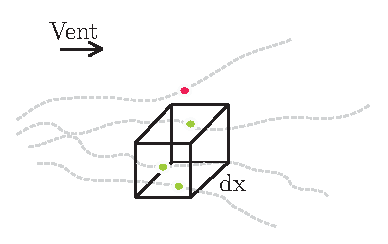
\includegraphics[width=0.65\textwidth]{lagrangian_ok}
	\caption{Principe du modèle lagrangien: la concentration en $\Vecx$ s'obtient par la somme des PL (en vert) traversant le volume élémentaire $d\Vecx$ durant un certain temps de résidence.}
	\label{fig_schema_lagrangien}
\end{figure}

Afin de calculer le champ d'écoulement auquel sont soumises les PL, plusieurs méthodes sont disponibles. Il est par exemple possible de résoudre les équations de la mécanique des fluides via un outil de simulation de type CFD, ce qui permet une modélisation fine des phénomènes physiques mis en jeu. Une autre possibilité consiste à avoir recours à une simulation dite \textit{CFD simplifiée}, où le champ de vent est interpolé à partir des mesures d'une ou plusieurs stations météorologiques tout en prenant en compte la topographie du terrain. C'est cette dernière approche qui est employée dans les outils de calcul du CEA et d'ARIA Technologies, et que nous présentons dans le chapitre suivant. \\

\subsection{La chaîne de calcul SWIFT-SPRAY}

L'outil \textit{Parallel Micro-SWIFT-SPRAY} (PMSS) est une chaîne de calcul constituée de deux éléments distincts: un outil de CFD simplifiée (SWIFT) et un modèle de dispersion lagrangien stochastique (SPRAY). Il est généralement appliqué dans des études à petite échelle (par exemple, au niveau d'un quartier), mais grâce à sa version parallèle, il a récemment été utilisé sur des domaines plus grands, à l'exemple du cas AirCity \cite{Moussafir2014} où le modèle a été exécuté sur l'ensemble de la ville de Paris.\\

\subsubsection{SWIFT}

Le modèle SWIFT permet de produire des champs de vent 3D en exploitant différents types de données météorologiques sur un même site (profils de vent et de température, stations de mesures, sorties de modèles météorologiques de prévision). Il permet notamment de prendre en compte la topographie du milieu, la présence d'obstacles tels que des bâtiments, l'occupation des sols ou encore l'influence de la stabilité atmosphérique. Son fonctionnement peut être résumé en quatre étapes :  \\

\begin{enumerate}
	\item Dans un premier temps, les mesures météorologiques reçues en entrée sont interpolées sur les différents points constituant une version discrétisée du domaine.
	\item Dans un deuxième temps, l'effet des obstacles présents dans le domaine sur l'écoulement sont modélisés via la création de zones spécifiques dans le voisinage de ces obstacles où le champ de vitesse est calculé de façon spécifique.
	\item La troisième étape consiste à ajuster le champ de vent en appliquant un principe de conservation de la masse.
	\item Enfin, la dernière étape consiste à calculer la turbulence intrinsèque à l'écoulement modélisé.\\
\end{enumerate}

\begin{figure}[h!]
	\centering
	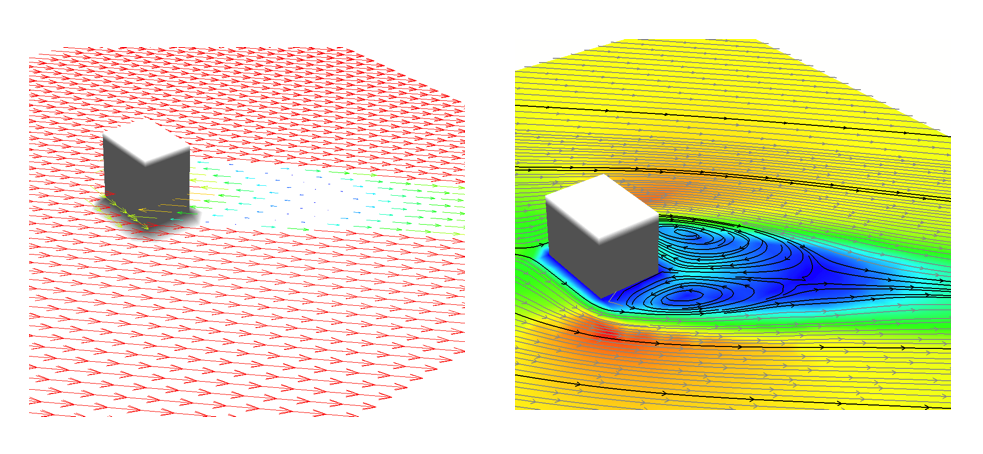
\includegraphics[width=0.75\textwidth]{swift_exemple}
	\caption{Exemple de calcul d'un champ de vent autour d'un obstacle avec SWIFT, avant (à gauche) et après (à droite) l'ajustement du champ}
	\label{fig_swift_exemple}
\end{figure}
En sortie de cet enchaînement de calculs, on obtient un champ de vent 3D qui peut alors directement être exploité par le modèle de dispersion SPRAY.



\subsubsection{SPRAY}

SPRAY est un modèle de dispersion lagrangien stochastique dont les principes de base suivent les mécanismes présentés à la section \ref{part_lagrangian}. L'implémentation de SPRAY repose sur le critère dit de \textit{well-mixed condition} permettant de donner une formulation explicite aux termes $a_i$ et $b_{i,j}$ de l'équation \eqref{eq_langevin} , et présenté en détail dans les travaux de \cite{Thomson1987}.

En pratique, plusieurs fonctionnalités supplémentaires sont implémentées dans SPRAY, telles que: \\

\begin{itemize}
	\item le "rebond" des particules sur les obstacles,
	\item le calcul de doses pour les sources radioactives,
	\item la prise en compte des différents types de dépôts (secs ou humides).\\
\end{itemize}

\begin{figure}[h!]
	\centering
	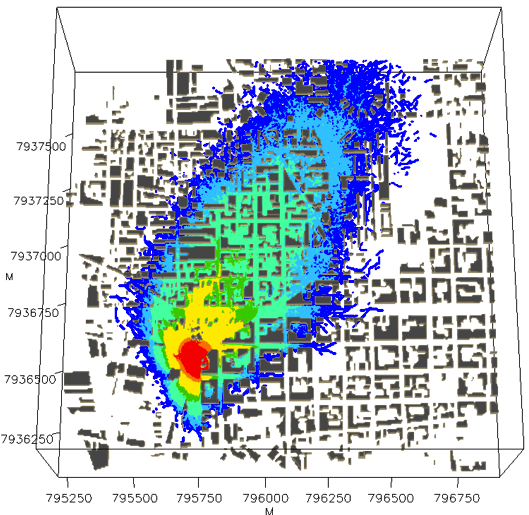
\includegraphics[width=0.65\textwidth]{spray_exemple}
	\caption{Exemple de champ de concentration calculé par SPRAY dans un domaine de type urbain}
	\label{fig_spray_exemple}
\end{figure}

La combinaison de SWIFT et SPRAY permet ainsi de calculer un champ de concentration sur le domaine étudié, connaissant les paramètres du terme source qui sont soumis en entrée du modèle SPRAY. Dans le contexte de ce chapitre, la chaîne de calcul PMSS permet de:

\begin{itemize}
	\item générer un jeu d'observations synthétiques en simulant un rejet induit par une source que l'on va chercher à retrouver: pour cela, on calcule les valeurs du champ de concentrations en un nombre fini de points du domaine que nous définirons comme étant les observations fournies par les capteurs,
	\item construire les matrices source-récepteur lors de l'exécution de l'algorithme AMIS, nécessaires au processus d'estimation du terme source.\\
\end{itemize}

\subsection{Dualité \textit{forward-backward}}

L'optimisation du calcul des matrices source-récepteur suivant le modèle de l'équation \eqref{eq_AE_4} est un point important: en effet dans une approche directe (\textit{forward}) telle que présentée dans le chapitre précédent, la construction des $\MatC(\VecTheta)$ pour chaque particule $\VecTheta$ échantillonnée depuis la loi de proposition courante fait appel à autant de calculs de dispersion, ce qui rend l'opération d'estimation du terme source très coûteuse en temps de calcul.\\

Nous proposons dans la suite de ce chapitre une amélioration du processus d'estimation privilégiant le calcul des matrices source-récepteur par une approche de type \textit{backward}. Cette méthodologie a initialement été introduite dans \cite{Keats2007} pour ensuite être appliquée sur un algorithme d'estimation de type MCMC, nous en rappelons les bases ci-après.\\

Soit une source ponctuelle $Q$ située au point de l'espace $\PosSource$, de débit massique constant $q_s$ et de temps d'activation et d'arrêt respectifs $t_{on}$ et $t_{off}$ définie par la distribution suivante:\\

\begin{equation}
	Q = q_s \delta(\Vecx - \PosSource)\left[H(t - t_{on}) - H(t - t_{off})\right]
\end{equation}
où $\delta$ est la distribution de Dirac et $H$ la fonction de Heaviside. On note $C$ le champ de concentration moyen induit par cette  source. La valeur simulée de concentration $c_i$ obtenue sur le $i$-ème capteur à l'instant $t$ peut se modéliser par l'équation suivante:

\begin{equation}
c_i = \int_0^t \int_V C h ~dtdV
\label{eq_int_direct}
\end{equation}
où $h$ est la \textit{fonction} de réponse du capteur. Cette équation peut se simplifier sous la notation suivante:\\

\begin{equation}
c_i = \langle	C,h\rangle
\label{eq_scal_direct}
\end{equation} 

La relation de \textit{dualité forward-backward} présentée par \cite{Keats2007} stipule que cette même concentration peut s'écrire sous la forme:

\begin{equation}
c_i = \int_0^t \int_V Q C^* ~ dtdV = \langle Q, C^*\rangle
\label{eq_int_adjoint}
\end{equation}
où $C^*$ est le champ de rétro-concentrations induit par le $i$-ème capteur, et dont les valeurs sont obtenues par la résolution de l'équation \eqref{eqn_advection_diffusion_backward}. Dans la pratique, le champ $C^*$ est simulé par un \textit{modèle de dispersion dual}, ou \textit{modèle de rétro-dispersion}.\\

La relation de dualité $\langle C,h\rangle = \langle Q,C^* \rangle$ est ainsi valable si l'équation duale d'advection-diffusion a été résolue de telle sorte que les conditions aux limites permettent d'annuler les termes de bord pouvant y apparaître. De plus:

\begin{enumerate}
	\item sous l'hypothèse d'un capteur idéal, sa résolution est infinie, ce qui se traduit en pratique par $h$ prenant la forme d'une distribution de Dirac,
	\item dans le cadre de la construction des matrices source-récepteur, $Q$ illustre une source instantanée et dont le débit de rejet est unitaire.
\end{enumerate}

Dans ce cas particulier, on obtient alors une équivalence entre $C$ et $C^*$: 

\begin{equation}
C \simeq C^*
\label{eq_equivalence}
\end{equation}


\subsection{Intégration d'un modèle \textit{backward} au processus d'estimation}

\subsubsection{Utilisation de RetroSPRAY dans l'AMIS}

L'outil PMSS dispose d'une version \textit{backward} de SPRAY appelée RetroSPRAY, dont l'intégration dans la chaîne de calcul se fait de la même façon que pour SPRAY. Le modèle RetroSPRAY procède à la résolution des équations de Langevin en mode inverse: 

\begin{equation}
\begin{split}
du_i^b &= U_i^b (t-dt) - U_i^b(t) \\
dx_i^b &= x_i^b (t-dt) - x_i^b(t)
\end{split}
\label{eq_langevin_inv1}
\end{equation}

On peut alors écrire l'équivalent inverse de l'équation \eqref{eq_langevin} sous la forme suivante:

\begin{equation}
	\begin{split}
	du_i^b &= a_i^b dt + b_{i,j}^b d\xi_j \\
	dx_i^b &= -(\bar{u}_i + U_i^b )dt
	\end{split}
	\label{eq_langevin_inv2}
\end{equation}

Les termes $a_i^b$ et $ b_{i,j}^b$ peuvent être calculés selon les expressions fournies dans \cite{Flesch1995} et \cite{Wilson2009}. \\

Si on examine plus en détail la construction de la matrice source-récepteur, on peut réécrire l'équation \eqref{eq_AE_4} sous une forme plus explicite: notons $C(R_i,t_j |\VecTheta, t'_n)$ la concentration moyenne au capteur $R_i$ à l'instant $t_j$ résultant d'une source située à la position $\VecTheta$ et ayant émis un rejet unitaire à l'instant $t'_n$. La version \textit{forward} de la matrice source-récepteur pour $\VecTheta$ s'écrit:

\begin{equation}
\MatC^f(\VecTheta) = 
\begin{pmatrix}
C(R_1,t_1 | \VecTheta, t'_1) & C(R_1,t_1 | \VecTheta, t'_2) & \cdots & C(R_1, t_1 |\VecTheta, t'_{T_s}) \\
C(R_1,t_2 | \VecTheta, t'_1) & C(R_1,t_2 | \VecTheta, t'_2) & \cdots & C(R_1, t_2 |\VecTheta, t'_{T_s}) \\
\vdots & \vdots & & \vdots \\
C(R_1,t_{T_c} | \VecTheta, t'_1) & C(R_1,t_{T_c} | \VecTheta, t'_2) & \cdots & C(R_1, t_{T_c} |\VecTheta, t'_{T_s}) \\
C(R_2,t_1| \VecTheta, t'_1) & C(R_2,t_1 | \VecTheta, t'_2) & \cdots & C(R_2, t_1 |\VecTheta, t'_{T_s}) \\
\vdots & \vdots & & \vdots \\
\vdots & \vdots & & \vdots \\
C(R_{N_c},t_{T_c} | \VecTheta, t'_1) & C(R_{N_c},t_{T_c} | \VecTheta, t'_2) & \cdots & C(R_{N_c}, t_{T_c} |\VecTheta, t'_{T_s}) \\
\end{pmatrix}
\label{eq_matrix_forward}
\end{equation}

En appliquant la relation de dualité \textit{forward-backward}, dans l'espace dual où le modèle \textit{backward} opère, les sources deviennent des "rétro-capteurs", et les capteurs deviennent des "rétro-sources". On définit alors $C^*(\VecTheta,t'_n | R_i, t_j)$ comme la rétro-concentration mesurée au point $\VecTheta$ à l'instant $t'_n$ provenant d'une rétro-source située à la position $R_i$ et ayant émis un rétro-rejet unitaire à l'instant $t_j$. La version \textit{backward} de $\MatC^f$ s'écrit alors:

\begin{equation}
\MatC^b (\VecTheta)= 
\begin{pmatrix}
	C^*(\VecTheta, t'_1 | R_1, t_1) & C^*(\VecTheta, t'_2 | R_1, t_1) & \cdots & C^*(\VecTheta, t'_{T_s} | R_1, t_1) \\
	C^*(\VecTheta, t'_1 | R_1, t_2) & C^*(\VecTheta, t'_2 | R_1, t_2) & \cdots & C^*(\VecTheta, t'_{T_s} | R_1, t_1) \\
	\vdots & \vdots & & \vdots \\
	C^*(\VecTheta, t'_1| R_1,t_{T_c}) & C^*(\VecTheta, t'_2 | R_1, t_{T_c}) & \cdots & C^*(\VecTheta, t'_{T_s} | R_1, t_{T_c}) \\ 
	\vdots & \vdots & & \vdots \\
	\vdots & \vdots & & \vdots \\
	C^*(\VecTheta, t'_1| R_{N_c},t_{T_c}) & C^*(\VecTheta, t'_2 | R_{N_c}, t_{T_c}) & \cdots & C^*(\VecTheta, t'_{T_s} | R_{N_c}, t_{T_c}) \\ 
	
\end{pmatrix}
\label{eq_matrix_backward}
\end{equation}

Dans l'algorithme AMIS, au moment de calculer la vraisemblance de chaque particule échantillonnée, on peut ainsi faire désormais intervenir $\MatC^b$ comme matrice source-récepteur.

\subsubsection{Avantages}

Le fait de substituer un modèle \textit{backward} au modèle \textit{forward} permet de n'avoir à faire qu'un seul calcul de rétro-dispersion par capteur, qui donne alors l'ensemble des valeurs de rétro-concentrations sur le domaine. De plus, ces calculs sont désormais opérés en amont du schéma itératif de l'AMIS: au lieu d'exécuter une boucle qui lance des calculs de dispersion pour chaque particule AMIS et à chaque itération, les champs $C^*$ sont pré-calculés et déjà disponibles au moment de l'estimation du terme source. \\

\begin{figure}[h!]
	\centering
	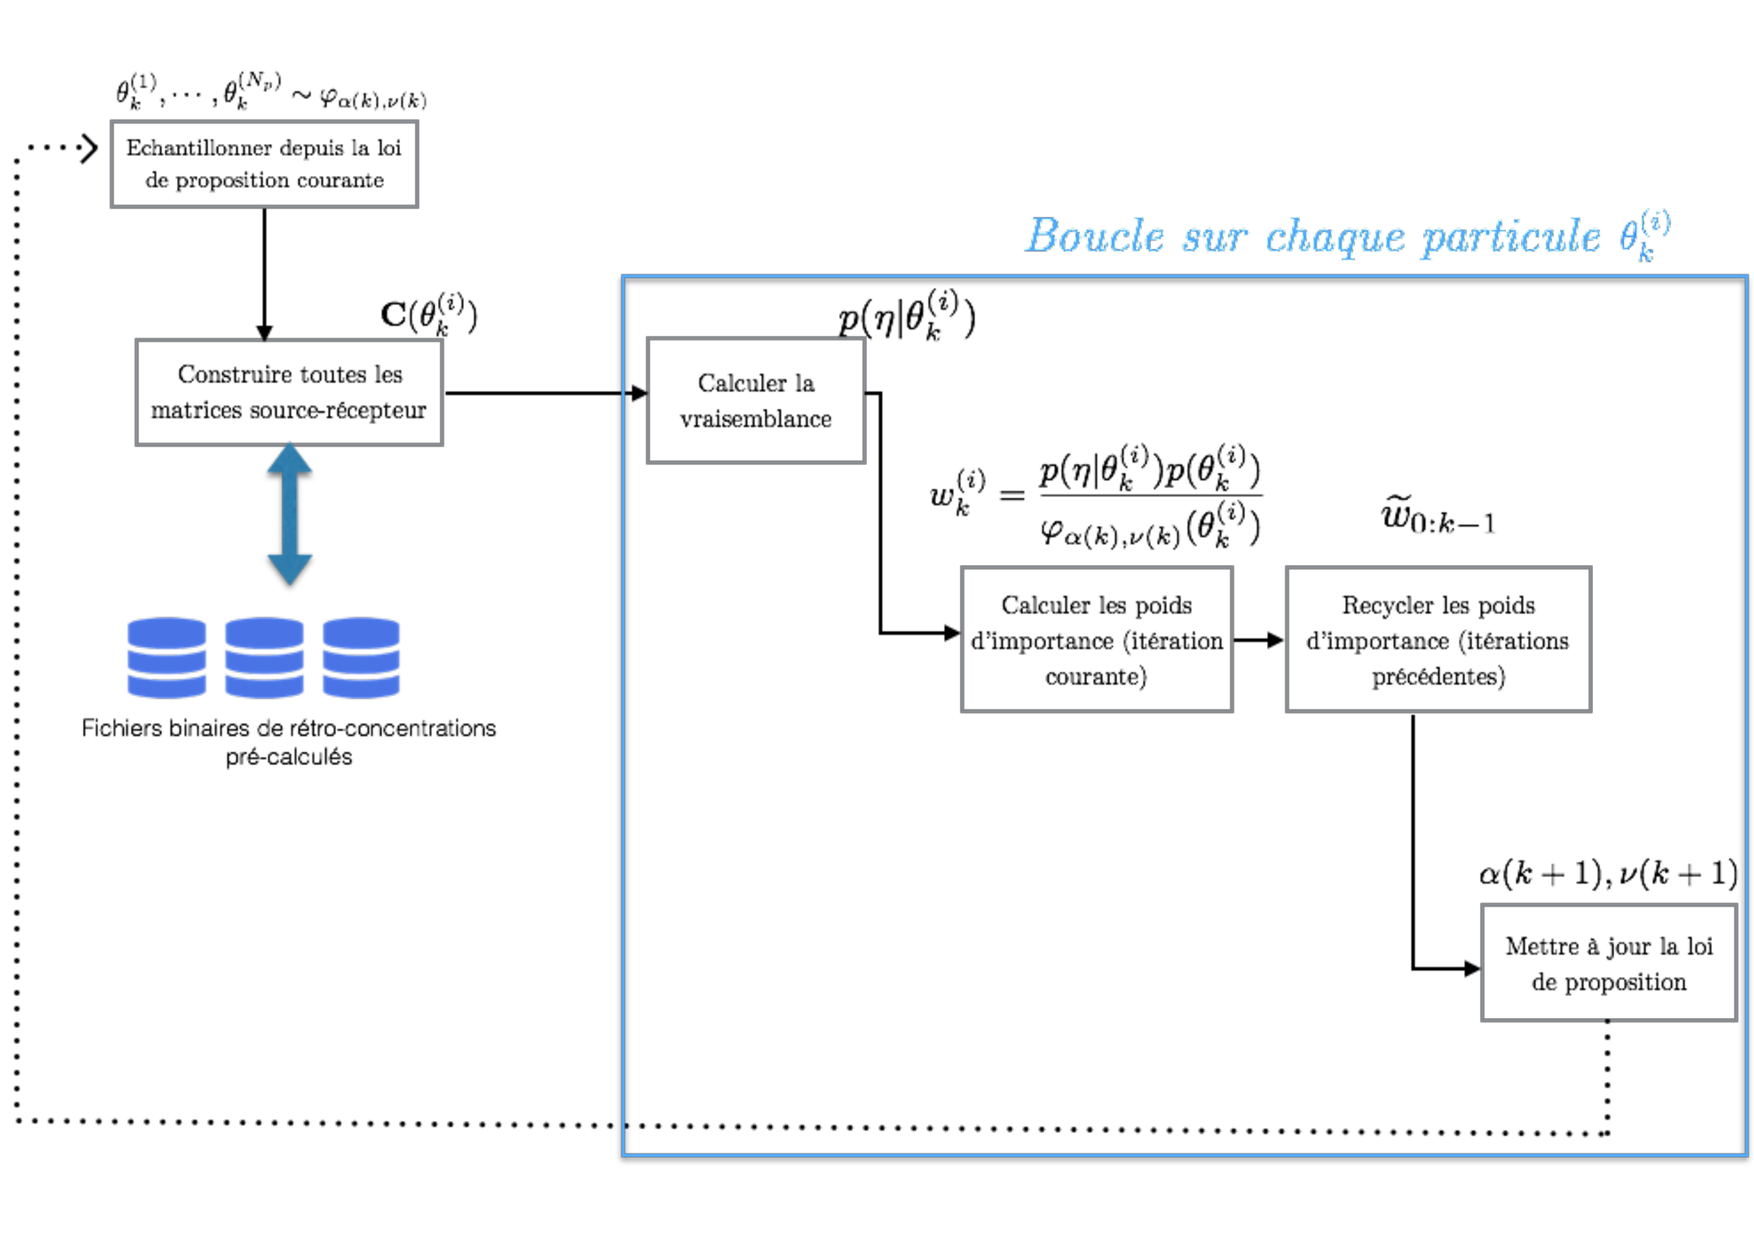
\includegraphics[width=0.75\textwidth]{schema_amis_optimise}
	\caption{Schéma de principe de la version \textit{backward} de l'algorithme d'estimation du terme source}
	\label{fig_schema_amis_optimise}
\end{figure}

Comme l'illustre la figure \ref{fig_schema_amis_optimise}, aucun calcul de dispersion n'est donc instancié durant la mise en oeuvre de l'algorithme, car les matrices source-récepteur sont désormais construites grâce à des opérations de lecture des fichiers dans lesquels ont été stockés les valeurs de $C^*$ pré-calculées. PMSS permet en effet d'agréger les résultats des calculs de dispersion dans des fichiers binaires, qui servent de base de données où les valeurs de rétro-concentration en chaque point du domaine peuvent être lues par un module d'entrée/sortie intégré à l'implémentation de l'AMIS.

Même si cette opération n'est plus directement intégrée à l'algorithme d'estimation, elle demande néanmoins une certaine quantité de calculs. Cette dernière peut toutefois être réduite si on choisit de paralléliser l'opération de génération des fichiers binaires de rétro-concentration. Comme il s'agit de tâches parfaitement indépendantes les unes par rapport aux autres, la parallélisation est facilement réalisable (\textit{embarrasingly parallel jobs}). Si on doit générer $n_b$ fichiers binaires en allouant $n_p$ coeurs de calcul par opération de génération, cela requiert la disponibilité de $n_b \times n_p$ coeurs. Si une telle quantité de ressources n'est pas immédiatement disponible, il peut être plus judicieux de créer séquentiellement ces fichiers binaires. L'approche séquentielle est également à privilégier si on ne dispose pas d'une architecture de type \textit{cluster} permettant une parallélisation massive. \\


Il est néanmoins important de rappeler que le fait d'associer le modèle \textit{backward} au modèle \textit{forward} constitue une approximation. En effet, la partie "diffusion" du processus de dispersion atmosphérique est aléatoire, et ne peut être parfaitement reproduite dans le cas dual pour une configuration identique du modèle \textit{forward}, créant ainsi un écart incompressible entre les champs $C$ et $C^*$. 

Cet écart peut être minimisé en utilisant un nombre de PL suffisamment grand pour modéliser les rétro-rejets. Il faut toutefois prendre garde à ne pas choisir une grandeur trop élevée, qui demanderait un temps de calcul trop important au modèle. 


\section{Exemple d'application en rase campagne}

Dans cette section nous présentons un première application sur une situation  simple dans un contexte non-urbain. Il s'agit d'un exemple synthétique dont les données et les paramètres sont issus d'une simulation ayant permis la validation du modèle RetroSPRAY.

\subsection{Présentation du cas-test}

Nous considérons ici un cas-test en milieu rural reproduisant une émission accidentelle depuis un site industriel dans une zone située près de la commune de Beaune, en Bourgogne, en présence d'une topographie réelle. 

\begin{figure}[h!]
	\centering
	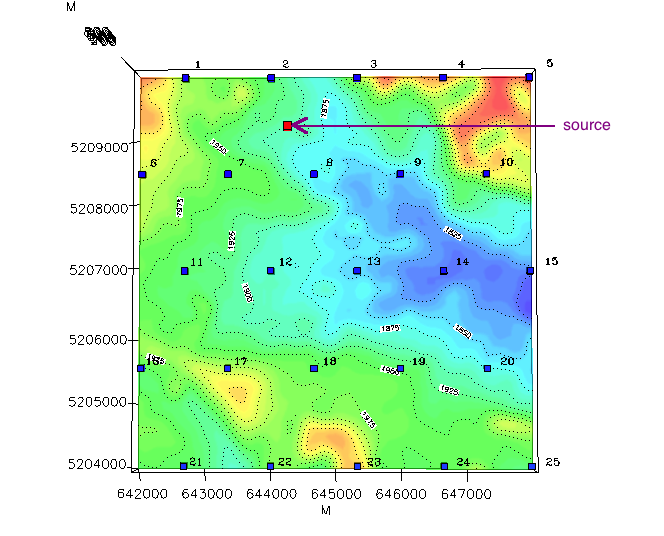
\includegraphics[width=0.8\textwidth]{beaune_relief_capteurs}
	\caption{Superposition du relief, de l'emplacement des capteurs et de la source du cas-test Beaune}
	\label{fig_beaune_relief}
\end{figure}

\subsubsection{Caractéristiques du domaine}
Le domaine considéré couvre une surface de \SI{6}{\square\kilo\meter} avec une source unique et un réseau relativement dense de 25 capteurs disposés en quinconce et couvrant toute la superficie du domaine (figure \ref{fig_beaune_relief}).

Pour la simulation, le domaine est discrétisé en une grille de $300 \times 300$ mailles, avec une résolution du maillage en $x$ et $y$ de \SI{20}{\meter}.

\subsubsection{Paramètres météorologiques}
Sur toute la durée de la simulation, nous considérons un vent constant en vitesse (\SI{1.5}{\m\per\second}) et en direction ($330\degres$). Le champ de vent produit par SWIFT est ainsi relativement homogène, comme observé en figure \ref{fig_beaune_vent}.

\begin{figure}[h!]
	\centering
	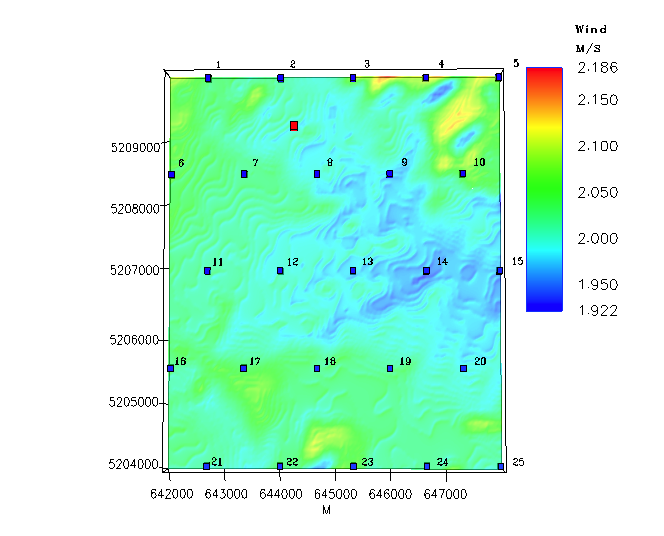
\includegraphics[width=0.8\textwidth]{beaune_vent}
	\caption{Champ de vent calculé par SWIFT pour le cas-test Beaune}
	\label{fig_beaune_vent}
\end{figure}


\subsubsection{Capteurs, source et simulation des observations}
On considère un réseau de 25 capteurs disposés de façon à couvrir tout le domaine, et placés à une hauteur de \SI{10}{\meter}, égale à celle de la source. Chaque capteur fournit des observations de concentrations moyennes entre 10h05 et 12h00, avec une plage de moyennage de 5 minutes.

Concernant la source, celle-ci est placée dans la partie nord (voir figure \ref{fig_beaune_relief}) afin que le panache résultant couvre une partie suffisante du domaine. Elle est située à une altitude de \SI{10}{\m}, identique à celle des capteurs: lors du processus d'estimation, on fait l'hypothèse que cette information est connue afin de limiter la reconstruction de la position aux coordonnées $(x,y)$. La source émet un rejet unique entre 10h15 et 11h, avec un débit constant de 1850 unités/s. \\

Il existe trois façons possibles de simuler le vecteur d'observation $\VecObs$ avec PMSS: 

\begin{enumerate}
	\item en spécifiant directement à SPRAY la position voulue pour la source ainsi que ses paramètres temporels d'émission,
	\item en calculant une matrice source-récepteur \textit{forward} $\MatC^f$ via SPRAY à la position voulue, puis en multipliant cette matrice par le profil d'émission $\VecQSource$ désiré,
	\item en calculant une matrice source \textit{backward} $\MatC^b$ via RetroSPRAY à la position voulue, puis en multipliant cette matrice par le profil d'émission $\VecQSource$ désiré.\\
	
\end{enumerate}

Si les représentations 1. et 2. sont équivalentes, la correspondance entre 2. et 3. n'est cependant pas immédiate : 

\begin{itemize}
	\item dans les configurations \textit{forward}, on définit un volume élémentaire $\Delta v_s^f$ pour la source et un volume de contrôle $\Delta v_c^f$ pour chacun des capteurs,
	\item dans le cas \textit{backward}, il faut également attribuer un volume élémentaire $\Delta v_s^b$ pour les rétro-sources et un volume de contrôle $\Delta v_c^b $ pour les points où sont simulés les concentrations conjuguées.\\
	
\end{itemize}

Pour avoir équivalence entre 2. et 3., il faut alors avoir: 

\begin{equation}
\begin{split}
\Delta v_s^f &= \Delta v_c^b \\
\Delta v_c^f &= \Delta v_s^b
\end{split}
\label{eq_dim_volumes}
\end{equation}

Or les paramètres d'origine de la simulation du cas-test Beaune spécifiaient des valeurs différentes pour $\Delta v_s^f$ (\SI{15}{\meter}$\times$\SI{15}{\meter}$\times$\SI{10}{\meter}) et $\Delta v_c^b$ (\SI{20}{\meter}$\times$\SI{20}{\meter}$\times$\SI{10}{\meter}) . Les résultats de la figure \ref{fig_comparaison_3_obs} reflètent ainsi les divergences engendrées par le non-respect des conditions \eqref{eq_dim_volumes}.

\begin{figure}[h!]
	\centering
	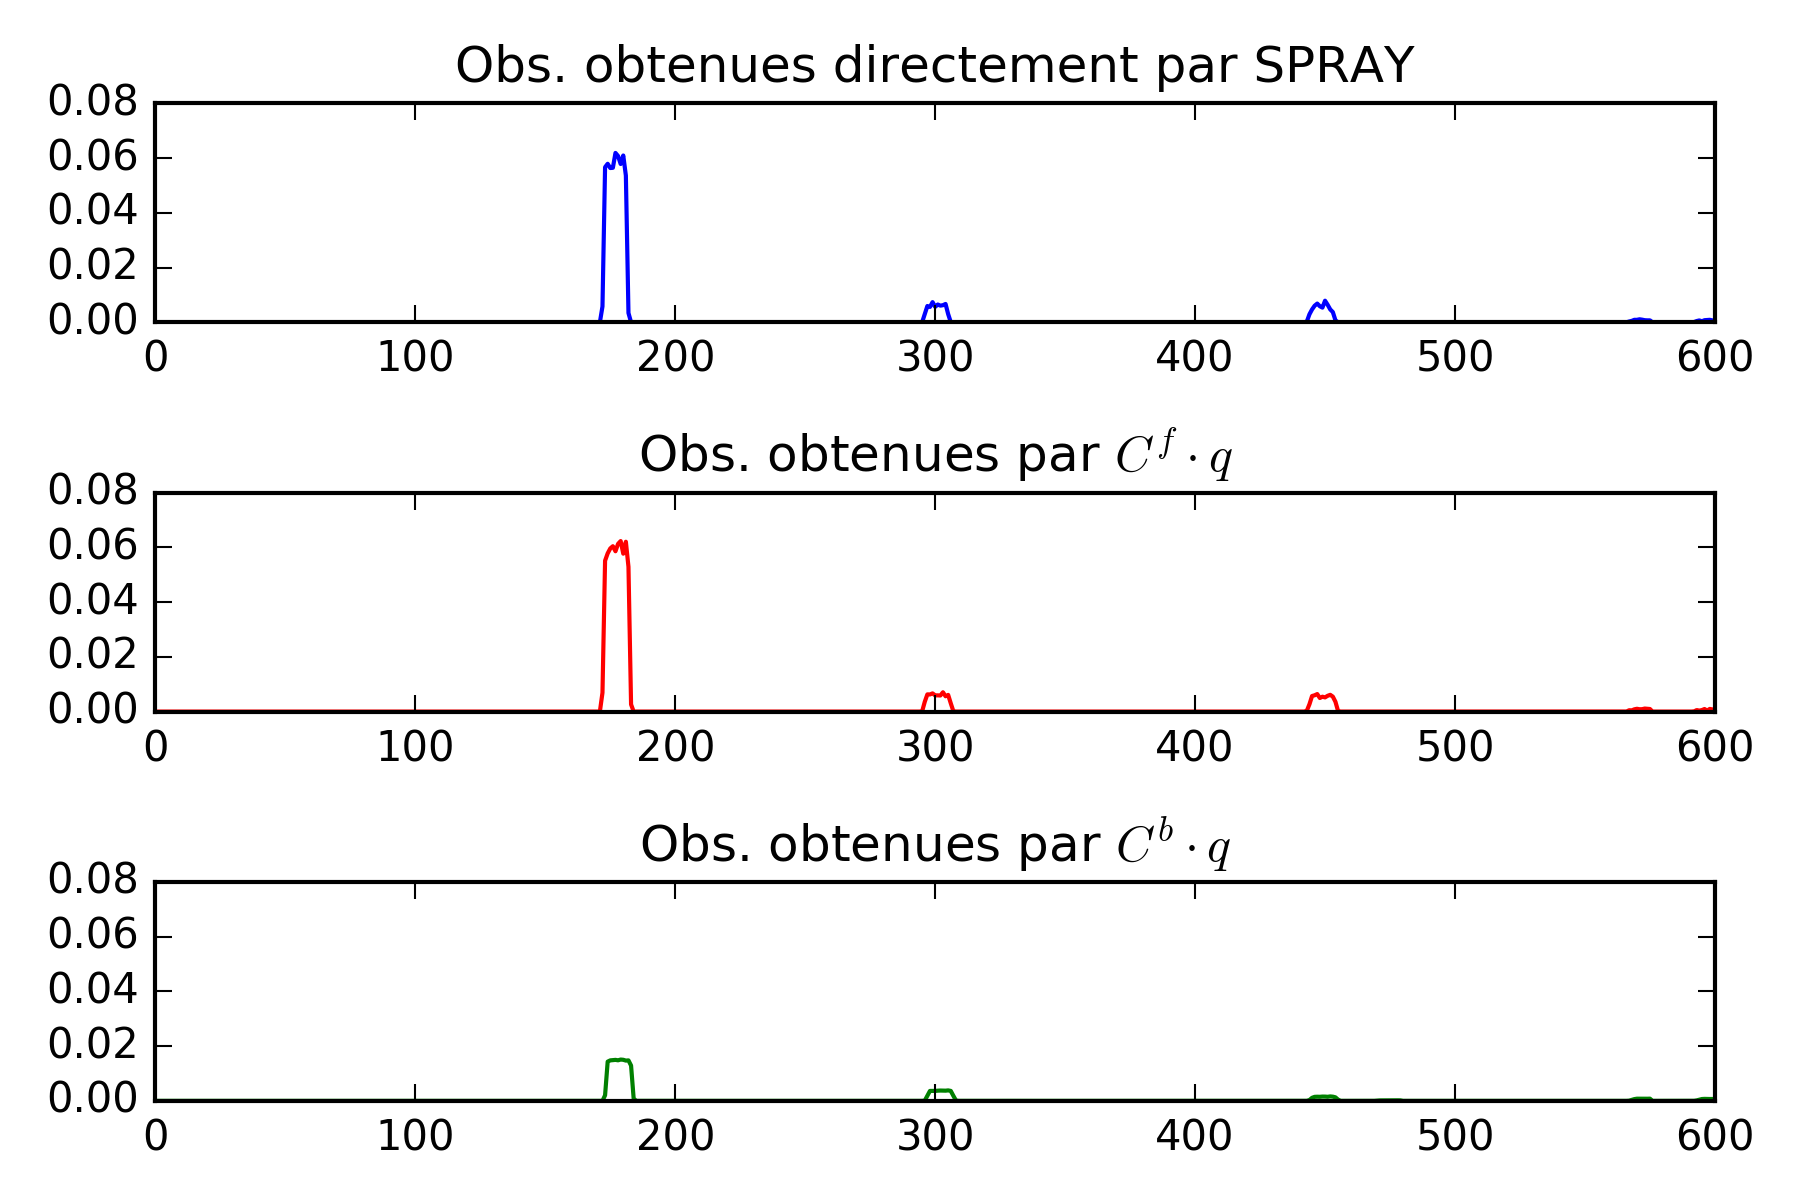
\includegraphics[width=0.8\textwidth]{comparaison_3_obs.png}
	\caption{Cas-test Beaune: différents modes de construction du vecteur $\VecObs$}
	\label{fig_comparaison_3_obs}
\end{figure}

Pour remédier à cela, on choisit alors de représenter la source comme un volume de dimension $\Delta v_c^b$ (autrement dit la source choisie couvre toute une maille du domaine), et d'utiliser la matrice source-récepteur \textit{backward} pour générer les observations. Cela permet en outre de s'assurer que la construction de $\VecObs$ est compatible avec la représentation des rétro-concentrations qui est utilisée dans l'algorithme d'estimation pour calculer la vraisemblance $p(\VecObs | \VecTheta)$ de chaque particule $\VecTheta$ tirée depuis la loi de proposition. Les mesures simulées par capteur sont représentées en figure \ref{fig_observations_25CAPTEURS}.

\begin{figure}[h!]
	\centering
	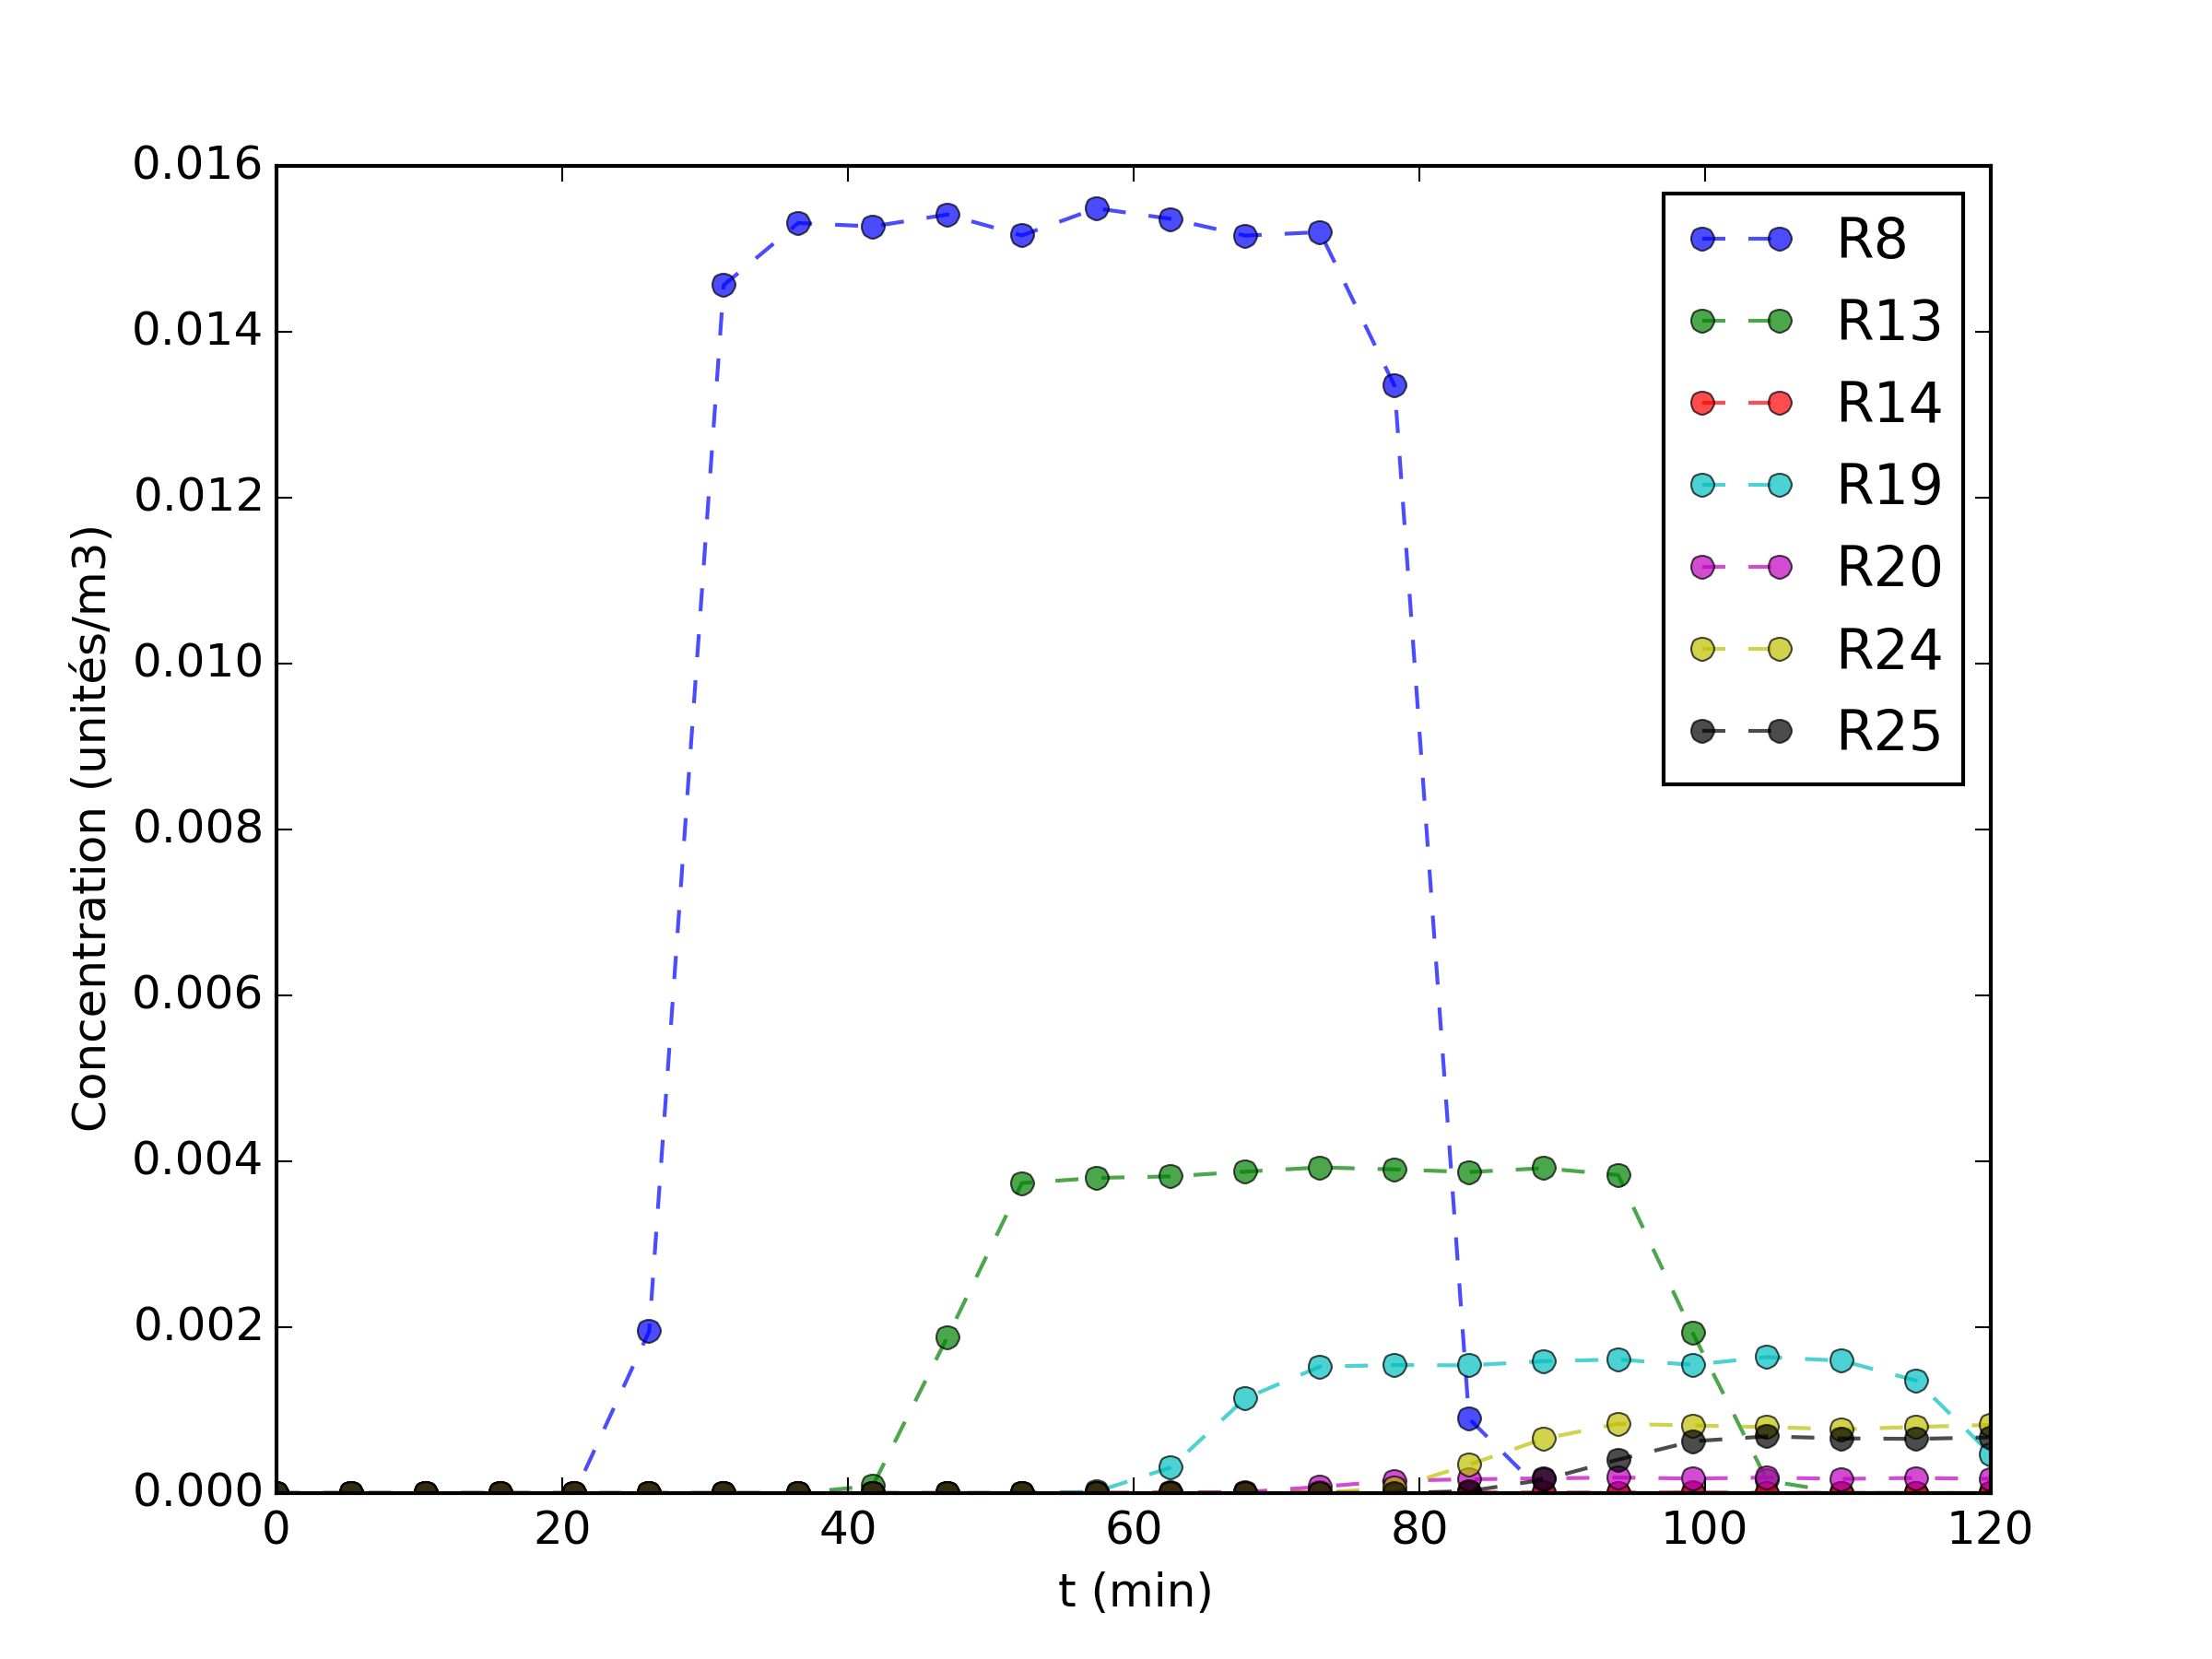
\includegraphics[width=0.8\textwidth]{concentrations_beaune.png}
	\caption{Cas-test Beaune: concentrations mesurées aux capteurs}
	\label{fig_observations_25CAPTEURS}
\end{figure}

\subsubsection{Premiers résultats}

Un \textit{run} préliminaire de l'AMIS servant de \textit{benchmark} a été lancé avec les paramètres suivants:
\begin{itemize}
	\item 10 itérations,
	\item 100 particules générées par itération,
	\item $\varObs = 2\times 10^{-6}$, qui fixe un degré d'incertitude suffisant autour des observations de la figure \ref{fig_observations_25CAPTEURS},
	\item une discrétisation temporelle de la source par paliers de 5 minutes, avec les paramètres a priori $\VecMeanQ = (0,\cdots,0)$ et $\varQ = 2\times 10^6$.
\end{itemize}

Avec ces paramètres, l'algorithme d'estimation parvient à fournir une reconstruction relativement correcte des paramètres, aussi bien concernant la localisation de la source (figures \ref{fig_25C_prelim_X} et \ref{fig_25C_prelim_Y}) que la reconstruction de son profil d'émission (figure \ref{fig_25C_prelim_Q}).\\

 \begin{figure}[h!]
 	\centering
 	\begin{subfigure}[t]{0.5\textwidth}
 		\centering
 		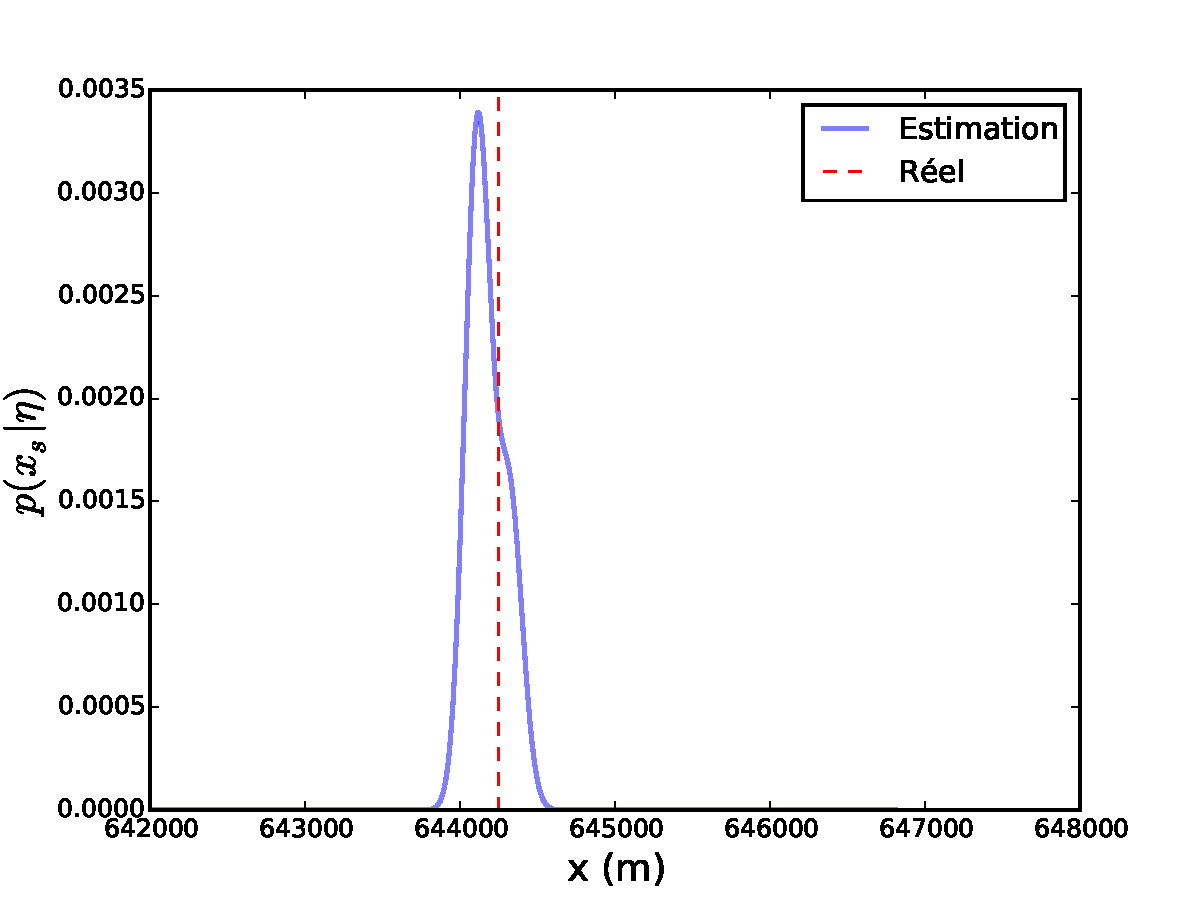
\includegraphics[width=1\textwidth]{beaune_25C_prelim_x}
 		\caption{Position en $x$}
 		\label{fig_25C_prelim_X}
 	\end{subfigure}%
 	\begin{subfigure}[t]{0.5\textwidth}
 		\centering
 		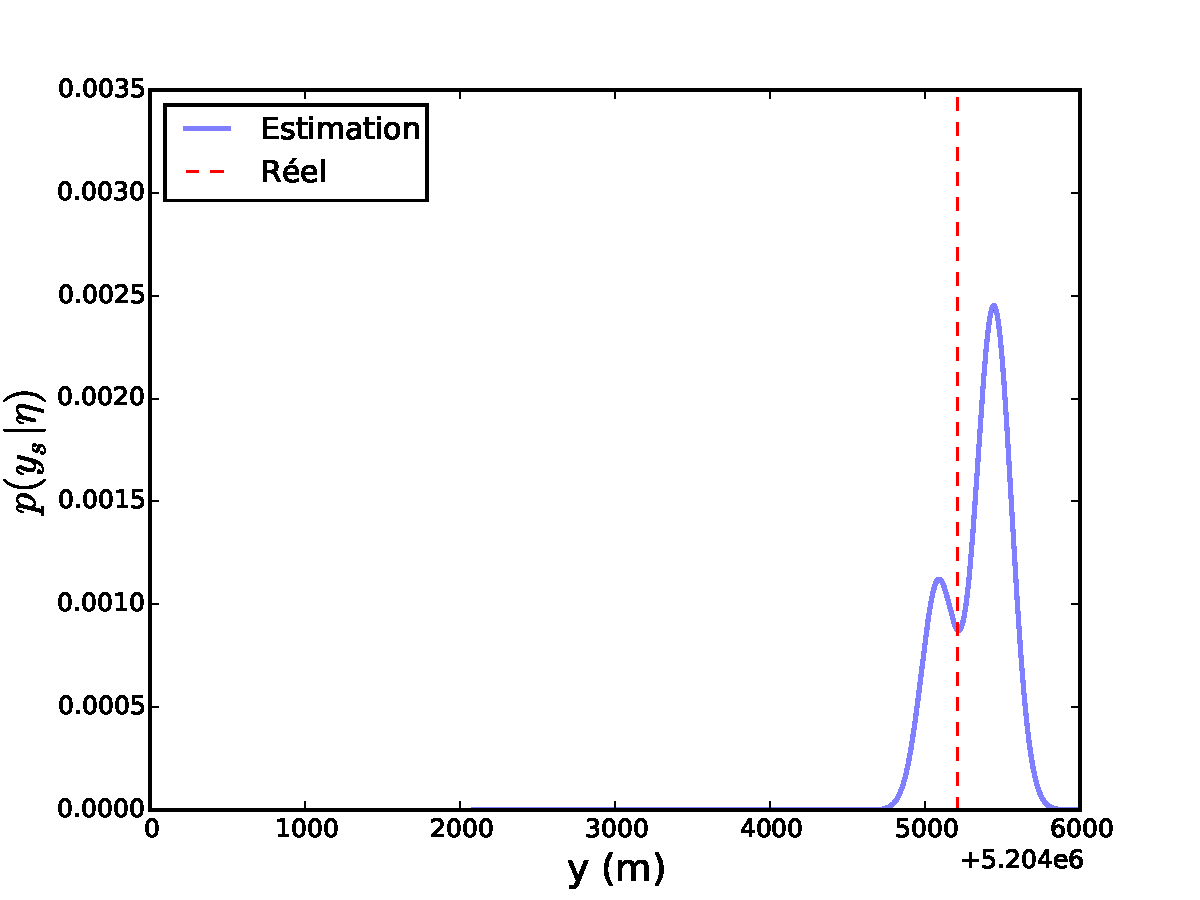
\includegraphics[width=1\textwidth]{beaune_25C_prelim_y}
 		\caption{Position en $y$}
 		\label{fig_25C_prelim_Y}
 	\end{subfigure}
 	\begin{subfigure}[t]{0.65\textwidth}
 		\centering
 		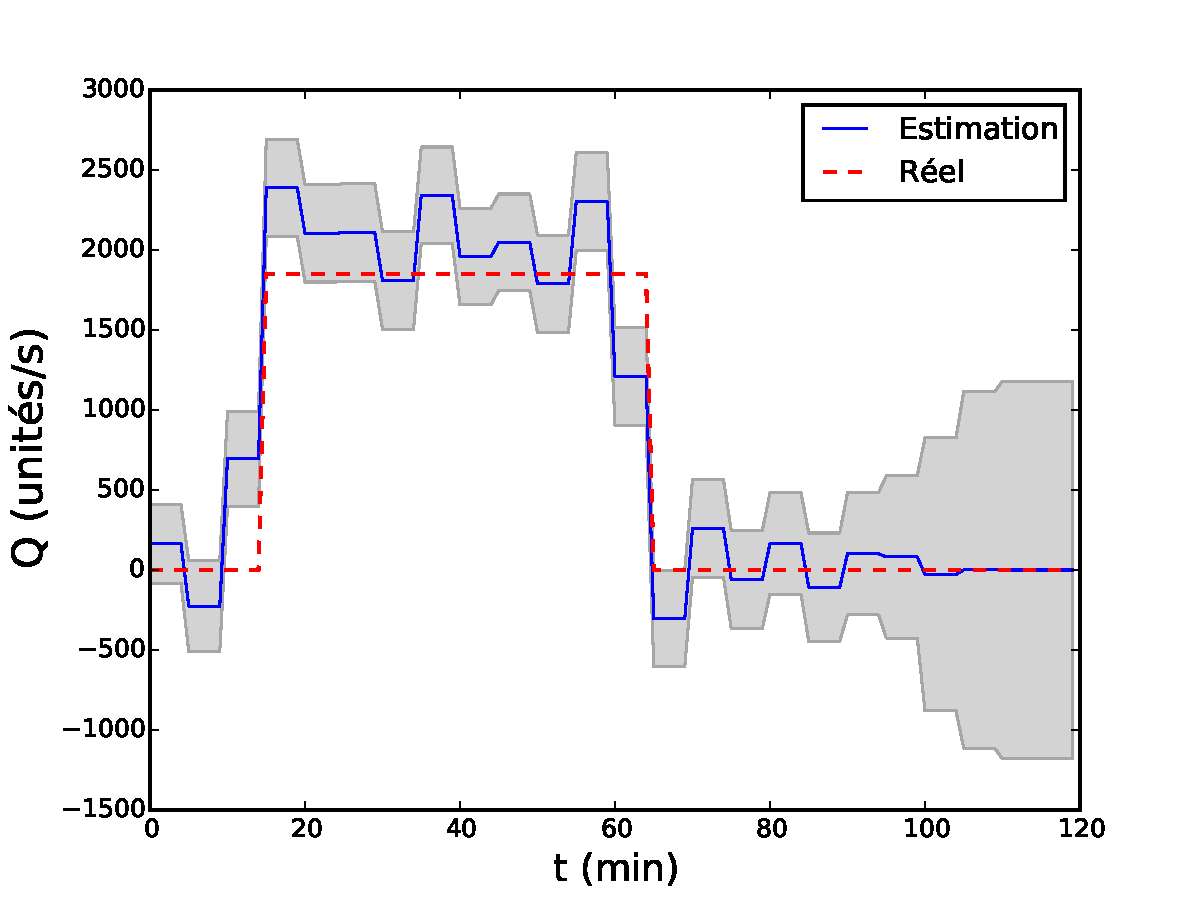
\includegraphics[width=1\textwidth]{beaune_25C_prelim_q}
 		\caption{Profil d'émission avec intervalle de confiance à  $\pm 2 \widetilde{\sigma}_q^2$ (gris)}
 		\label{fig_25C_prelim_Q}
 	\end{subfigure} 
 	\caption{Résultats du \textit{benchmark} de l'algorithme d'estimation sur le cas-test Beaune}
 	\label{fig_25C_prelim}
 \end{figure}
 
 Pour mesurer l'erreur relative d'une estimation ponctuelle par rapport à la vraie position de la source, on utilise la métrique suivante:
 
 \begin{equation}
	 r_d = \dfrac{d(\Vecx_s,\widehat{\Vecx}_{MMSE})}{L_{\mathcal{D}}}
 \end{equation}
 où:
 \begin{itemize}
 	\item $L_{\mathcal{D}}$ est la diagonale du domaine $\mathcal{D}$ considéré, autrement dit la plus grande distance possible entre deux points: cela permet de borner $r_d$ entre 0 et 1,
 	\item $\Vecx_s$ est le centre de la maille où est située la source,
 	\item $\widehat{\Vecx} _{MMSE}$ est l'estimation ponctuelle par MMSE de la position de la source obtenue via les particules et les poids d'importance fournis en sortie de l'AMIS.
 \end{itemize}
 
 Pour mesurer l'erreur d'estimation du débit, on utilise l'erreur quadratique moyenne définie par:
 \begin{equation}
	 Err(\tilde{\VecMeanQ}) = \dfrac{1}{T_s} \sum\limits_{i=1}^{T_s}(\VecQSource^{(i)} - \tilde{\VecMeanQ}^{(i)})^2
 \end{equation}
 où $\VecQSource$ est le profil d'émission réel et $\tilde{\VecMeanQ}$ est le profil estimé.\\
 
 Dans l'exemple de la figure \ref{fig_25C_prelim}, on obtient ainsi une erreur relative de $r_d = 0.017$ pour la position, et une erreur d'estimation du débit de $Err(\tilde{\VecMeanQ}) = 296.909$. \\
 
 Nous étudions dans les paragraphes suivants l'influence des paramètres de variance d'observation $\varObs$ et de variance a priori $\varQ$ du profil d'émission $\VecQSource$ sur la qualité de l'estimation. Une telle étude paramétrique permet en effet de donner du sens à ces paramètres, ceux-ci devant être spécifiés par l'utilisateur parmi les variables d'entrée de l'algorithme d'estimation. 
 
 \subsection{Influence de la variance d'observation}
 
 La variance d'observation $\varObs$ est le paramètre qui reflète la "confiance" donnée aux observations $\VecObs$. Comme expliqué au Chapitre 3, elle caractérise l'ensemble des erreurs à l'origine de l'écart entre les valeurs issues du modèle de données et la réalité physique. Comme il a été expliqué précédemment, l'erreur d'observation est une agrégation de diverses sources individuelles d'erreur (modèle, instrumentation...). Sans chercher à mener une analyse approfondie sur la quantification des incertitudes autour des observations, nous cherchons plutôt ici à avoir une vision d'ensemble de l'influence du paramètre $\varObs$ sur la qualité de l'estimation du terme source. Pour cela, on garde les mêmes paramètres que le \textit{benchmark} de la figure \ref{fig_25C_prelim}, on choisit ensuite une plage de valeurs de $\varObs$ à tester, et pour chacune de ces valeurs, on lance 100 \textit{runs} de l'AMIS. Ce dernier faisant intervenir des tirages aléatoires, le fait de considérer les résultats issus d'un nombre suffisant de \textit{runs} permet de voir si la qualité des estimations n'est pas perturbée par ces aspects stochastiques. Les valeurs de variance choisies sont $10^{-7}, 5\times 10^{-7}, 10^{-6}, 5\times 10^{-6}, 10^{-5}, 5\times 10^{-5},10^{-4}$. \\
   
         Concernant la localisation de la source, on observe sur les figures \ref{fig_25C_analyse_varobs_x} et \ref{fig_25C_analyse_varobs_y} de l'Annexe A que les résultats sont plutôt réguliers: l'estimation de la position est bonne pour les valeurs inférieures à $5\times 10^{-6}$ puis se dégrade progressivement jusqu'à avoir du mal à définir une zone précise de l'espace (\ref{varF_x} et \ref{varF_y}).
         
         Pour le profil d'estimation sur la figure \ref{fig_25C_analyse_varobs_q} de l'Annexe A, celui-ci est relativement bien estimé pour $\varObs=10^{-7}$, les variations étant de plus en plus importantes au fur et à mesure que la valeur de la variance d'observation augmente. Les courbes d'erreur de la figure \ref{fig_25C_varobs_erreurs} donnent un aperçu de l'influence générale de la variance d'observation.
         
         \begin{figure}[h!]
         	\centering
         	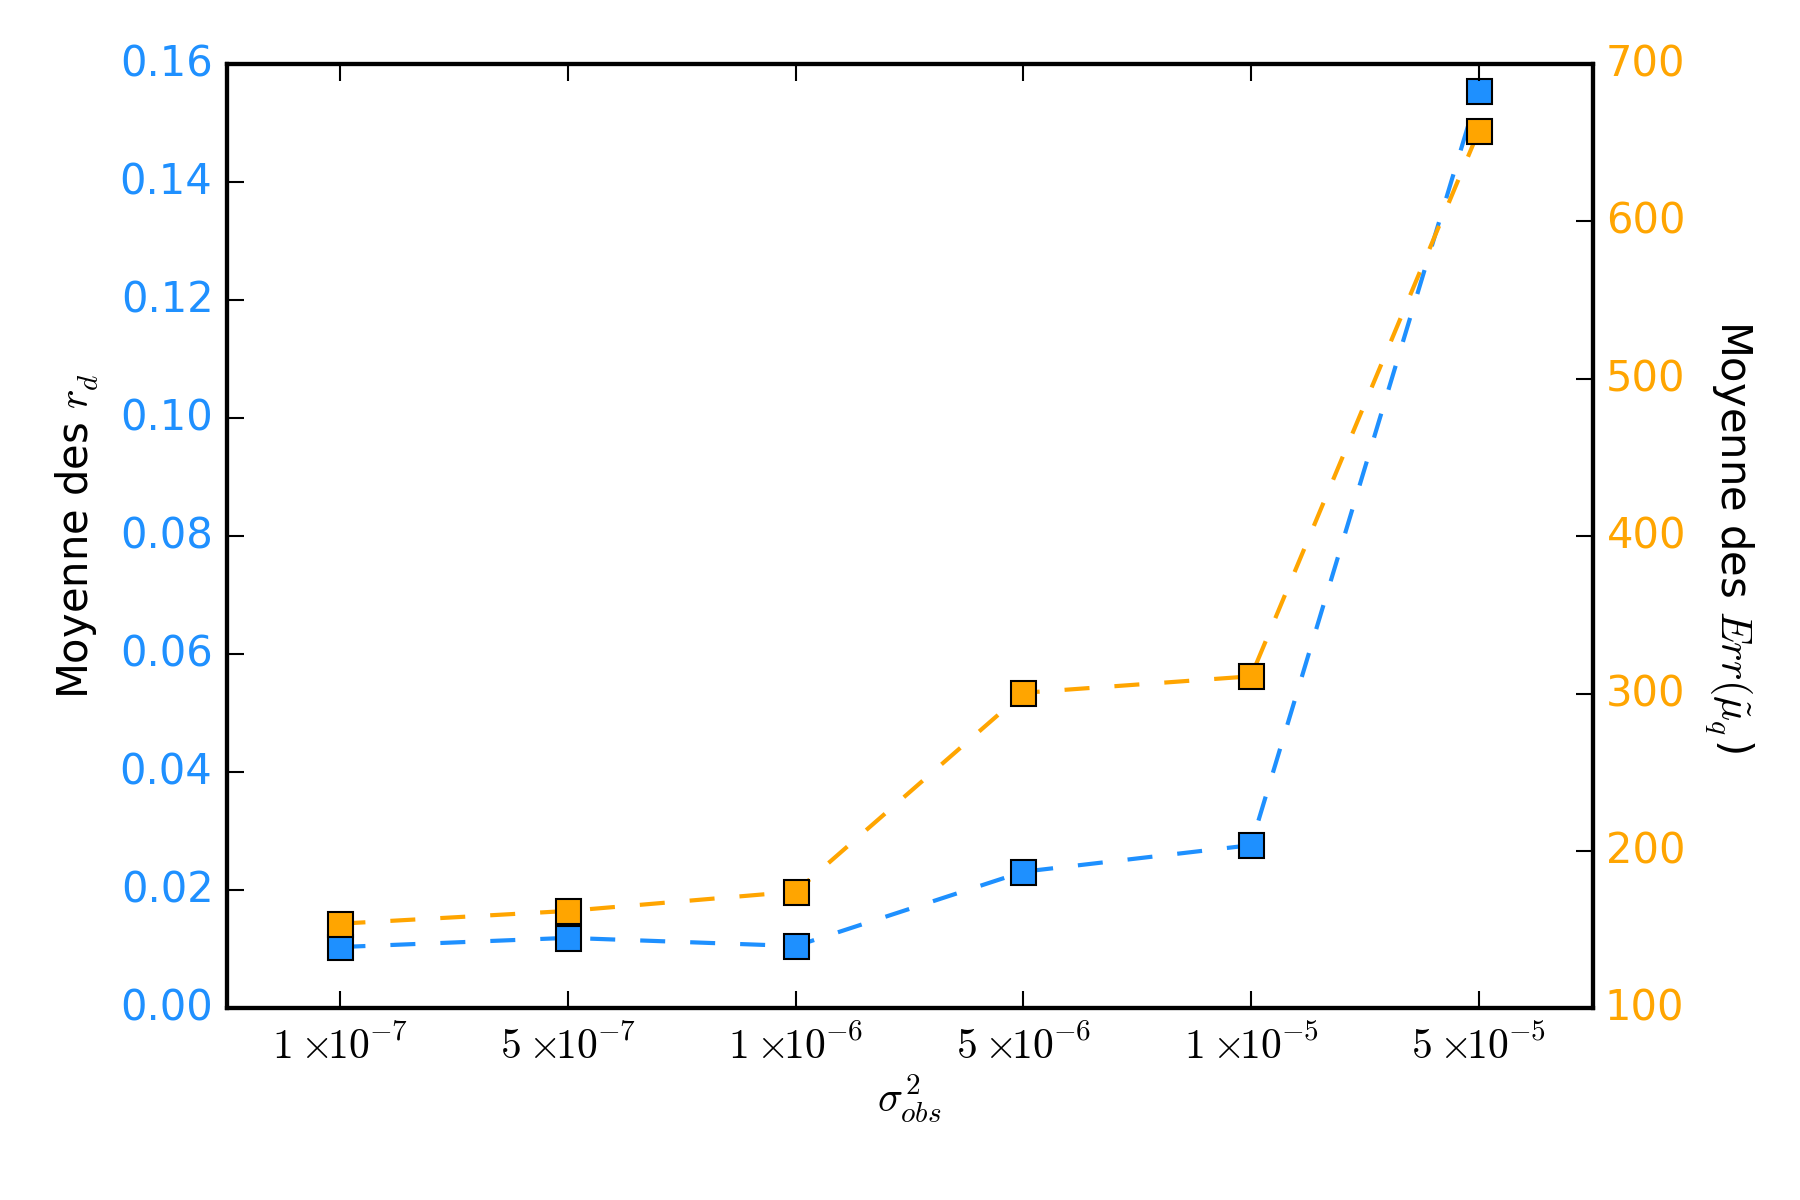
\includegraphics[width=0.8\textwidth]{25C_varobs_errors.png}
         	\caption{Courbes d'erreur pour l'analyse paramétrique de $\varObs$}
         	\label{fig_25C_varobs_erreurs}
         \end{figure}
         
         
         Certaines des valeurs estimées pour le débit soient négatives, or il a été constaté que l'application de la contrainte de positivité a tendance à surestimer les valeurs de $\tilde{\VecMeanQ}$, comme le montre l'exemple de la figure \ref{fig_sansavecPC}. Il a donc été décidé de ne pas implémenter cette contrainte, car malgré la présence de quelques valeurs négatives, le sens physique des résultats d'estimation est globalement respecté.
       
\begin{figure}[h!]
    	\centering
         	\begin{subfigure}[t]{0.5\textwidth}
         		\centering
         		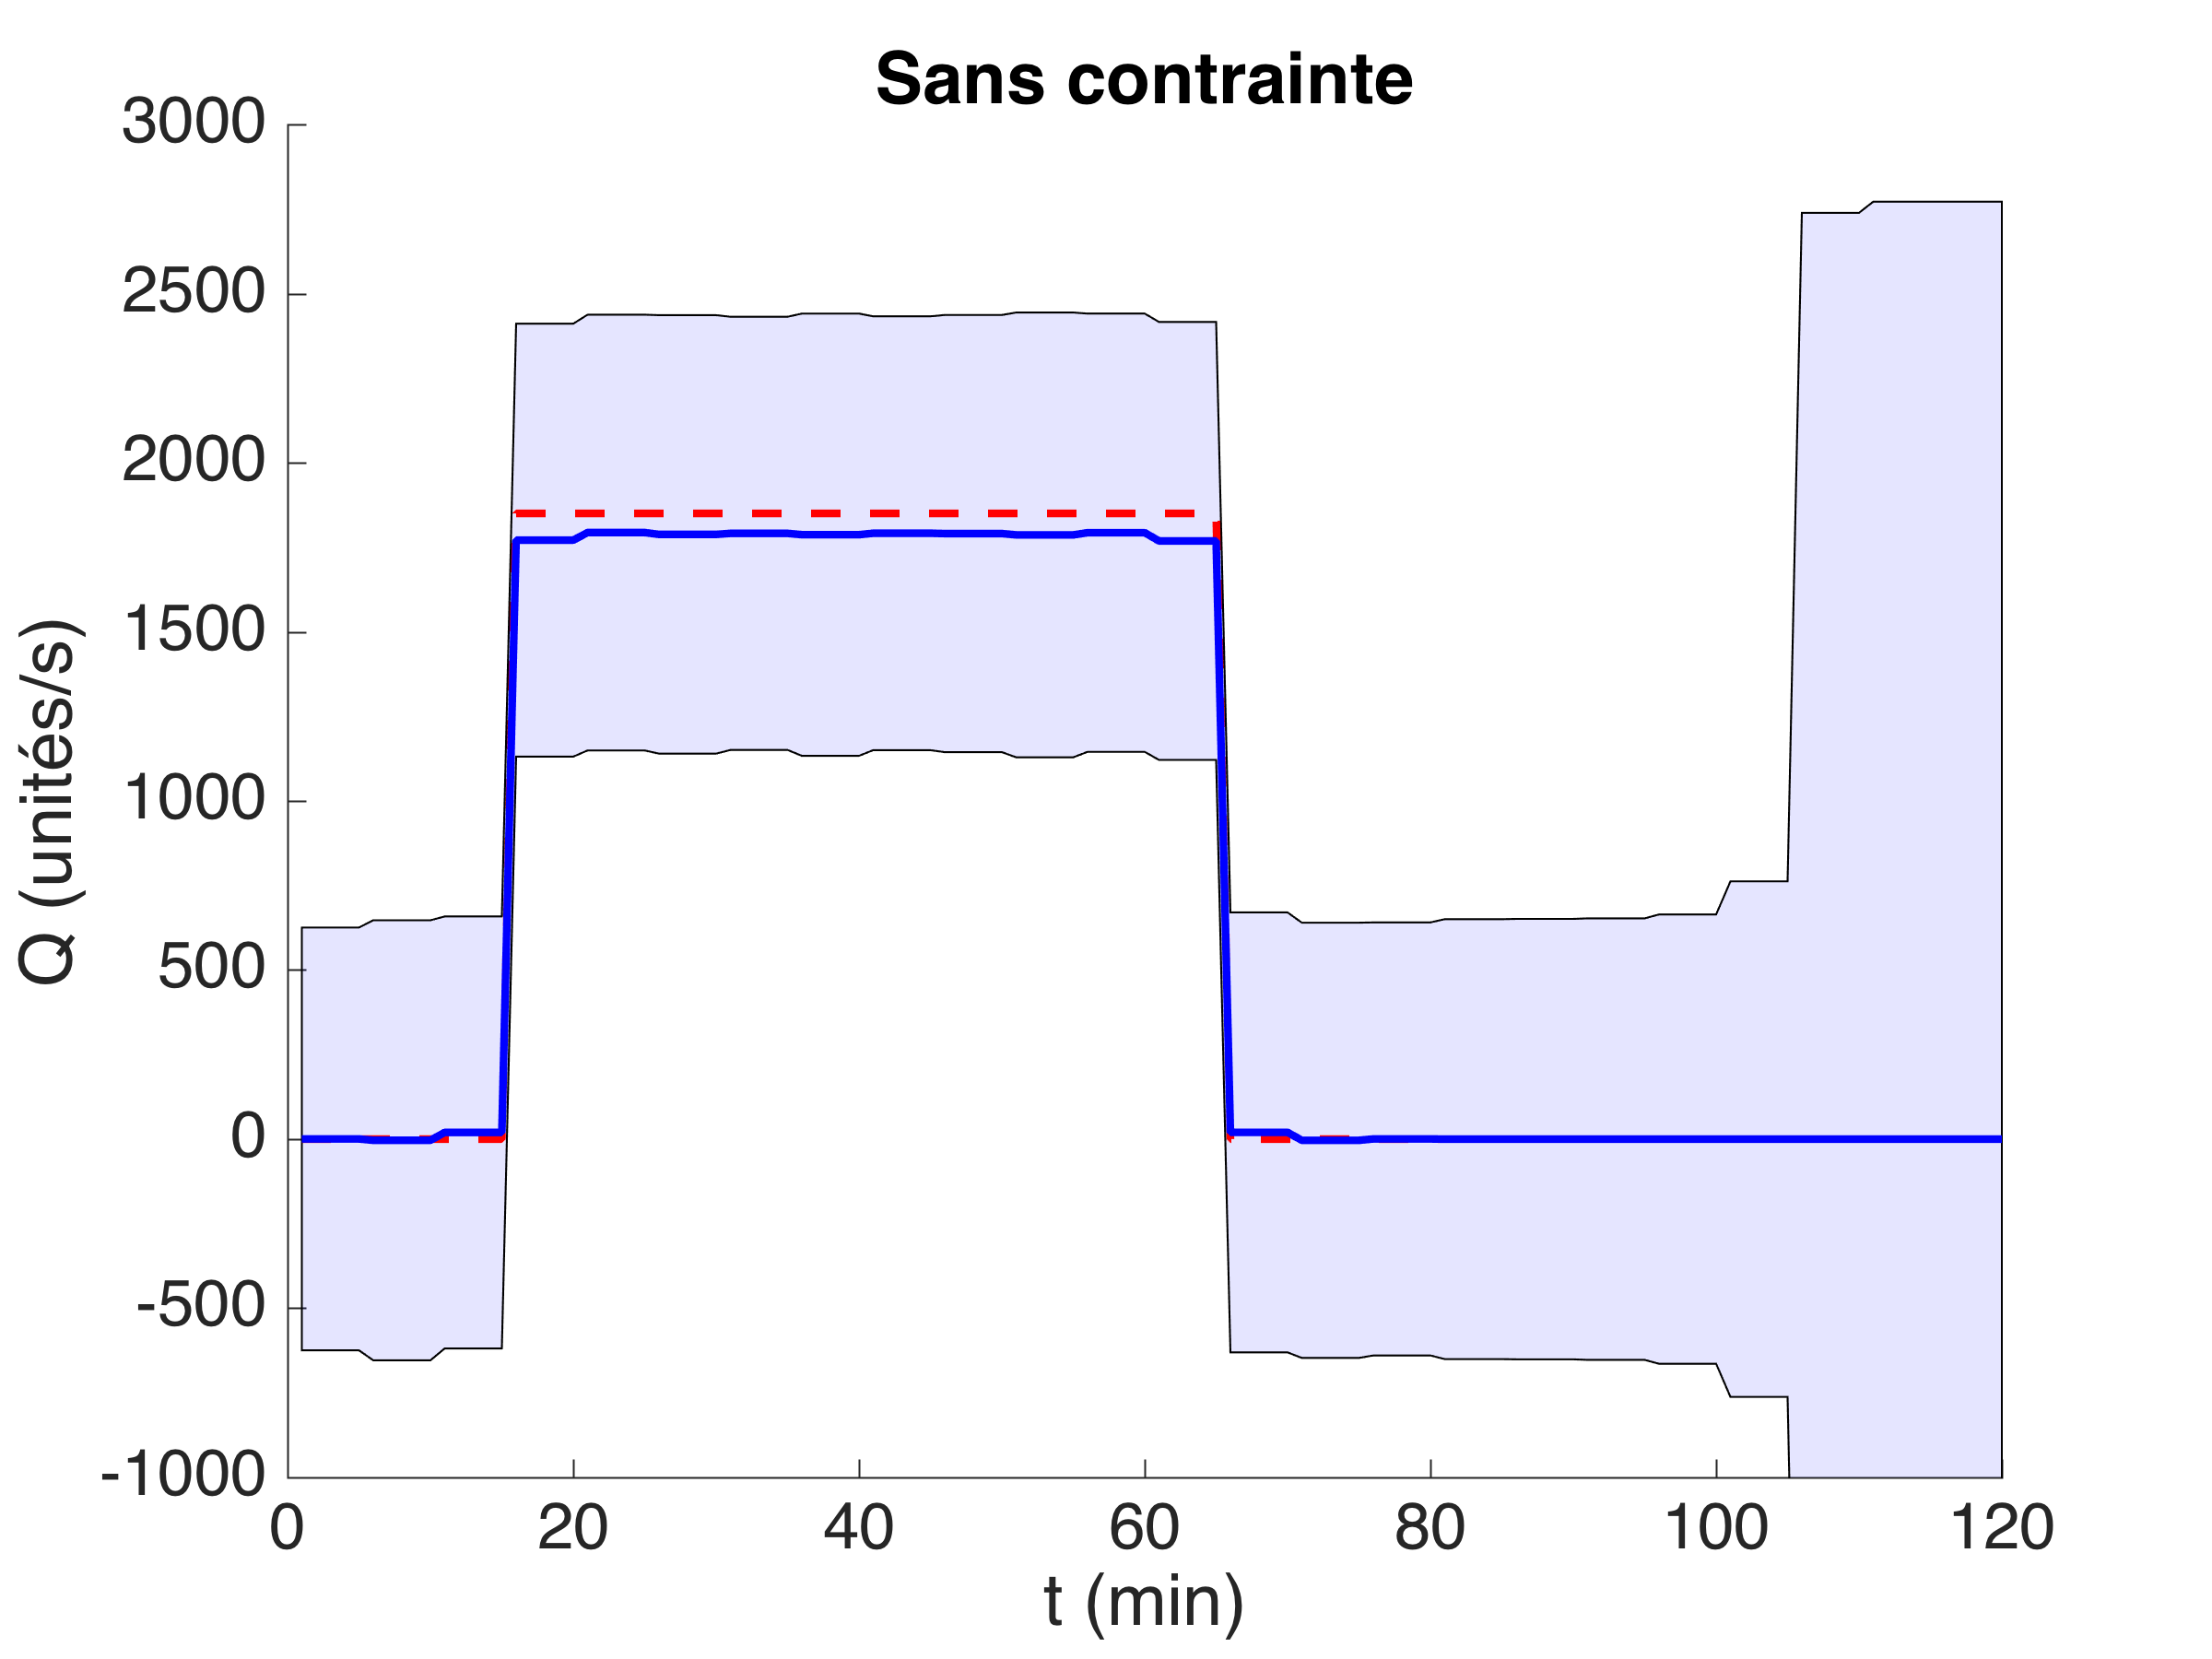
\includegraphics[width=1\textwidth]{1part_sansPC.png}
         		\caption{}
         		\label{sansPC}
         	\end{subfigure}%
         	\begin{subfigure}[t]{0.5\textwidth}
         		\centering
         		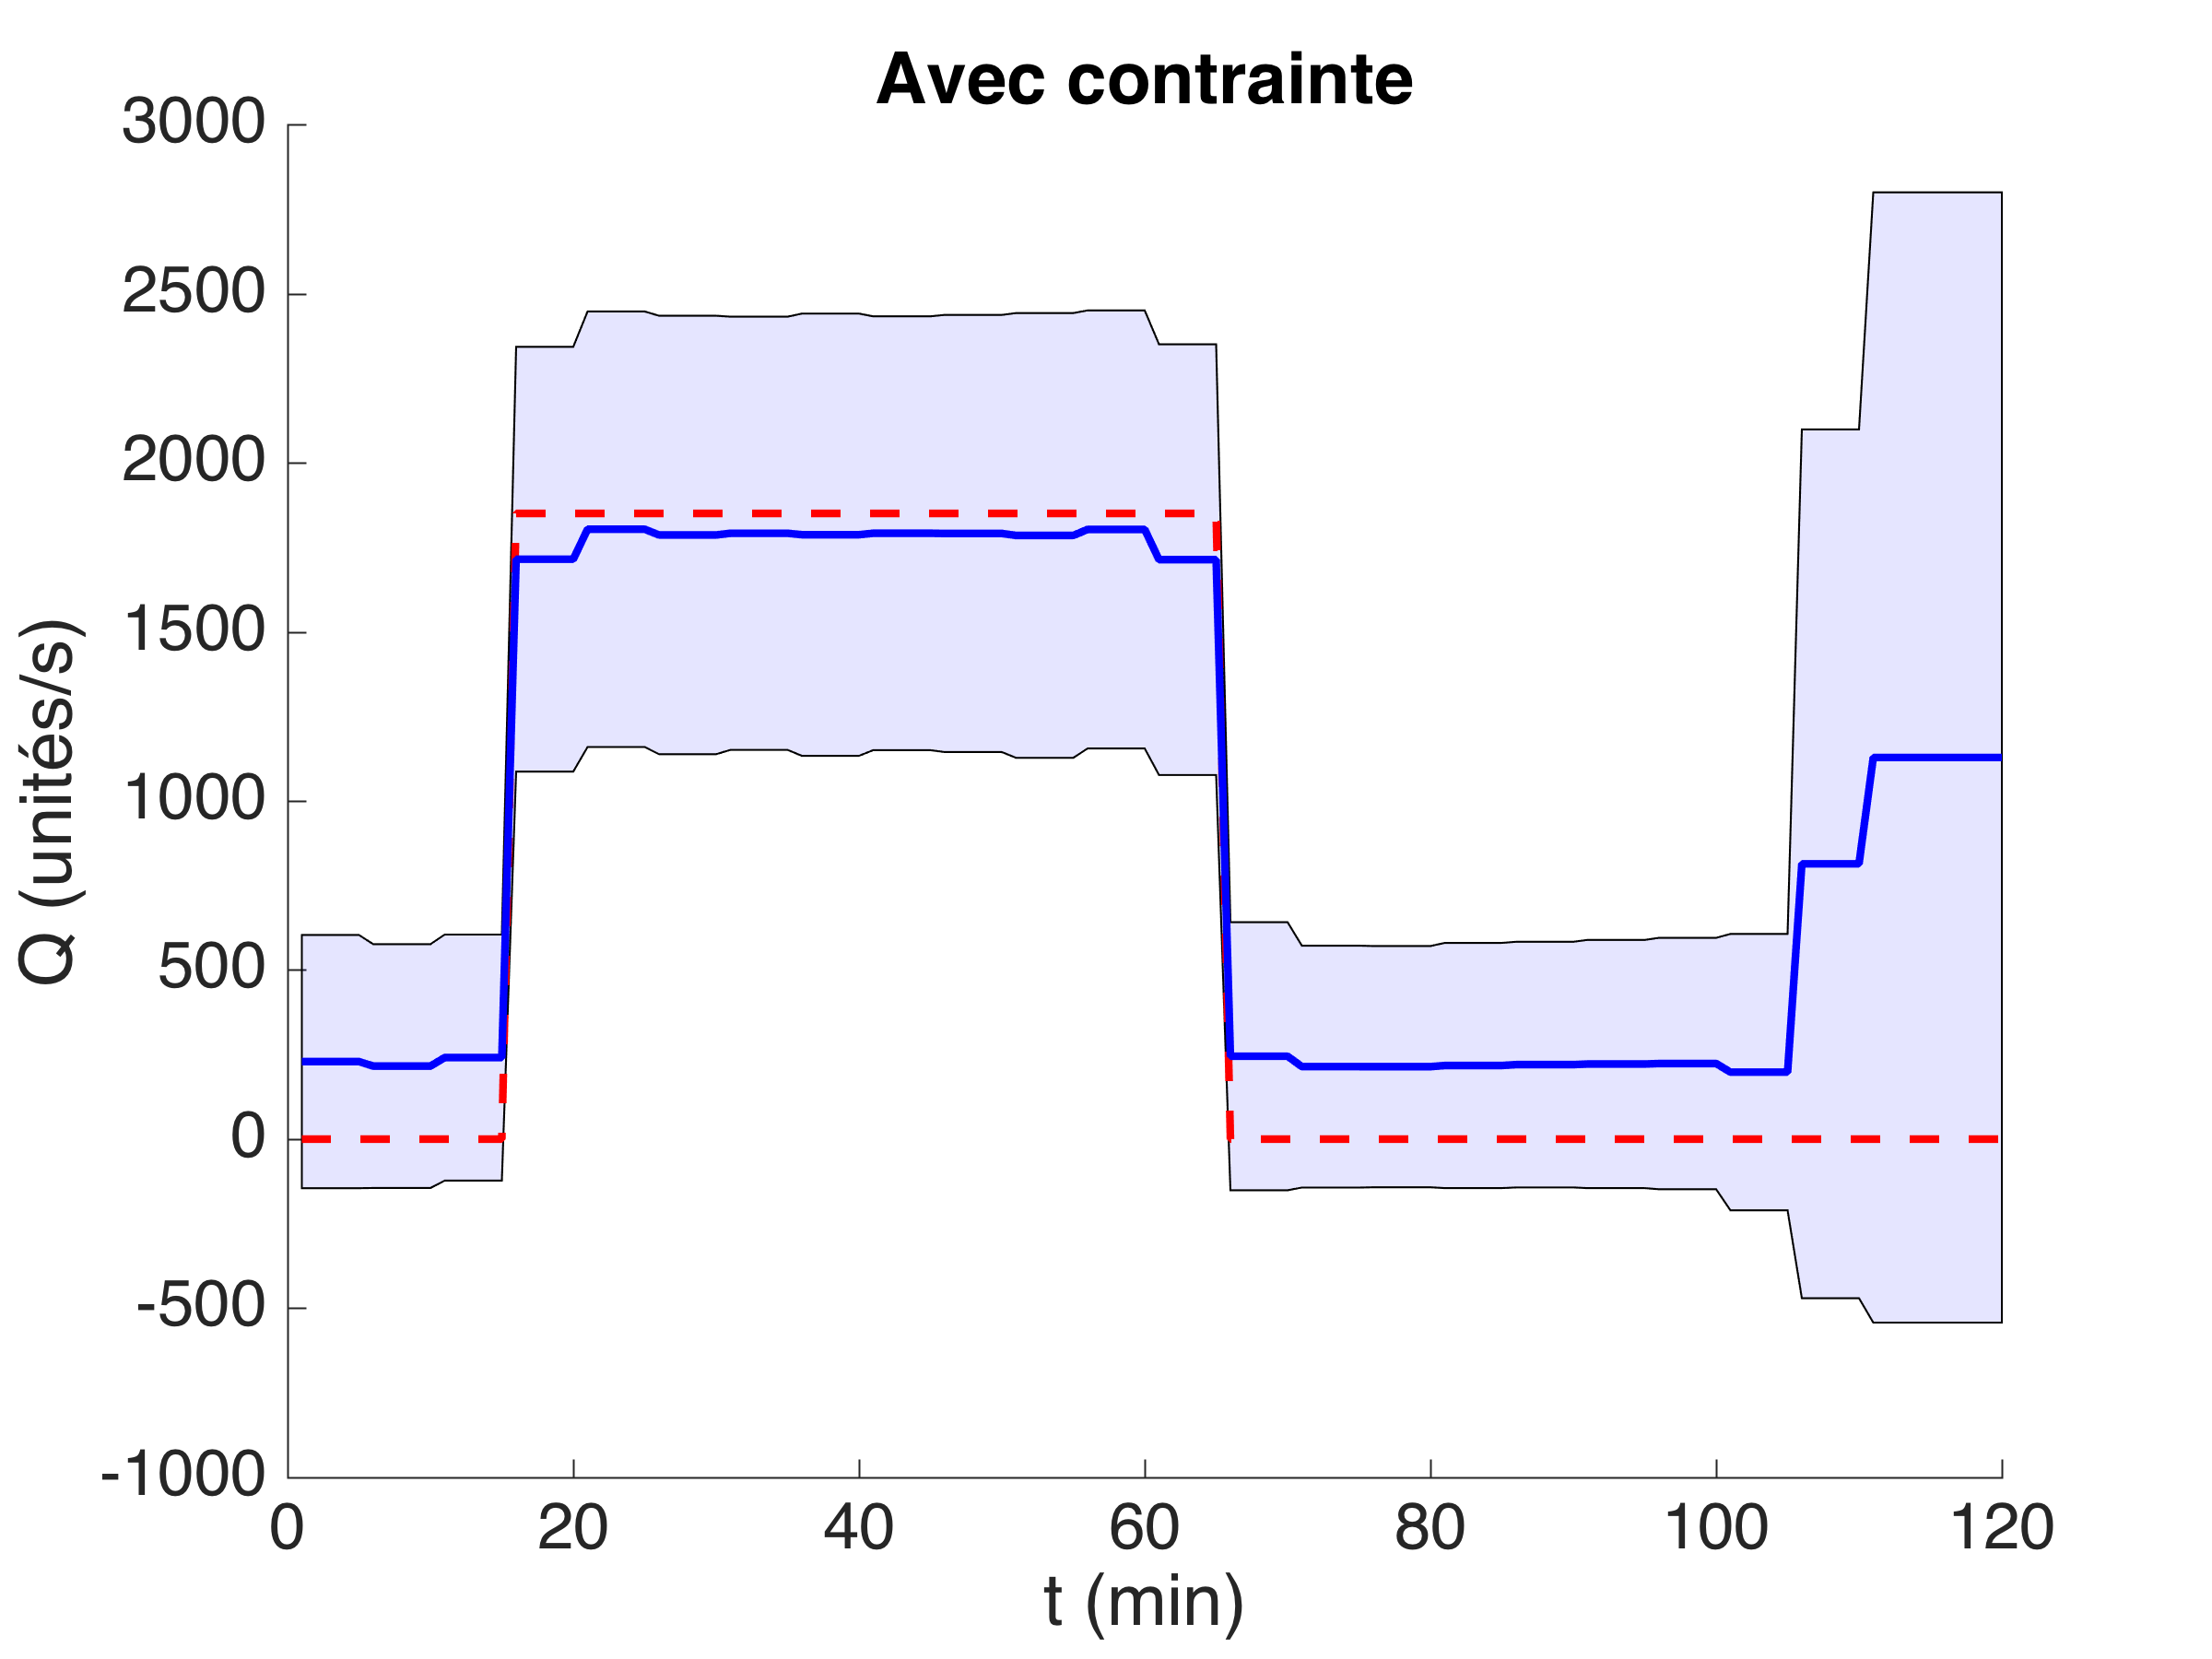
\includegraphics[width=1\textwidth]{1part_avecPC.png}
         		\caption{}
         		\label{avecPC}
         	\end{subfigure}
         	\caption{Comparaison de l'estimation de $\tilde{\VecMeanQ}$ sur une particule dans la maille de la source sans (à gauche) et avec (à droite) la contrainte de positivité}
         	\label{fig_sansavecPC}
         \end{figure}

En examinant les résultats des figures précédentes, on pourrait considérer la valeur $\varObs = 10^{-7}$ comme étant celle qui donne les meilleurs résultats. Il faut cependant rappeler que dans notre cas d'étude, nous utilisons des observations synthétiques non-bruitées, ce qui permet d'accorder une plus grande confiance à ces observations et donc de réduire la valeur de $\varObs$. On ne peut pas forcément en faire autant si des sources d'incertitudes supplémentaires entrent en jeu, par exemple avec des valeurs de concentrations expérimentales issues de mesures réelles, car cela reviendrait à diminuer la marge d'incertitude sur les mesures alors que le caractère aléatoire de ces dernières est plus accentué. 
%
%Pour illustrer le rôle de l'incertitude des mesures dans le choix du paramètre $\varObs$, on perturbe le vecteur d'observation $\VecObs$ avec un bruit additif gaussien centré, et pour préserver la cohérence physique de la simulation, on ramène les observations bruitées négatives à 0. L'intensité de la perturbation du signal d'observation est ainsi caractérisée par la variance du bruit $\varBruit$ choisie: on considère ici 3 différents niveaux dont l'impact sur $\VecObs$ est illustré par la figure \ref{fig_25_obs_noisy}.\\
%\begin{figure}[h!]
%	\centering
%	\begin{subfigure}[t]{0.33\textwidth}
%		\centering
%		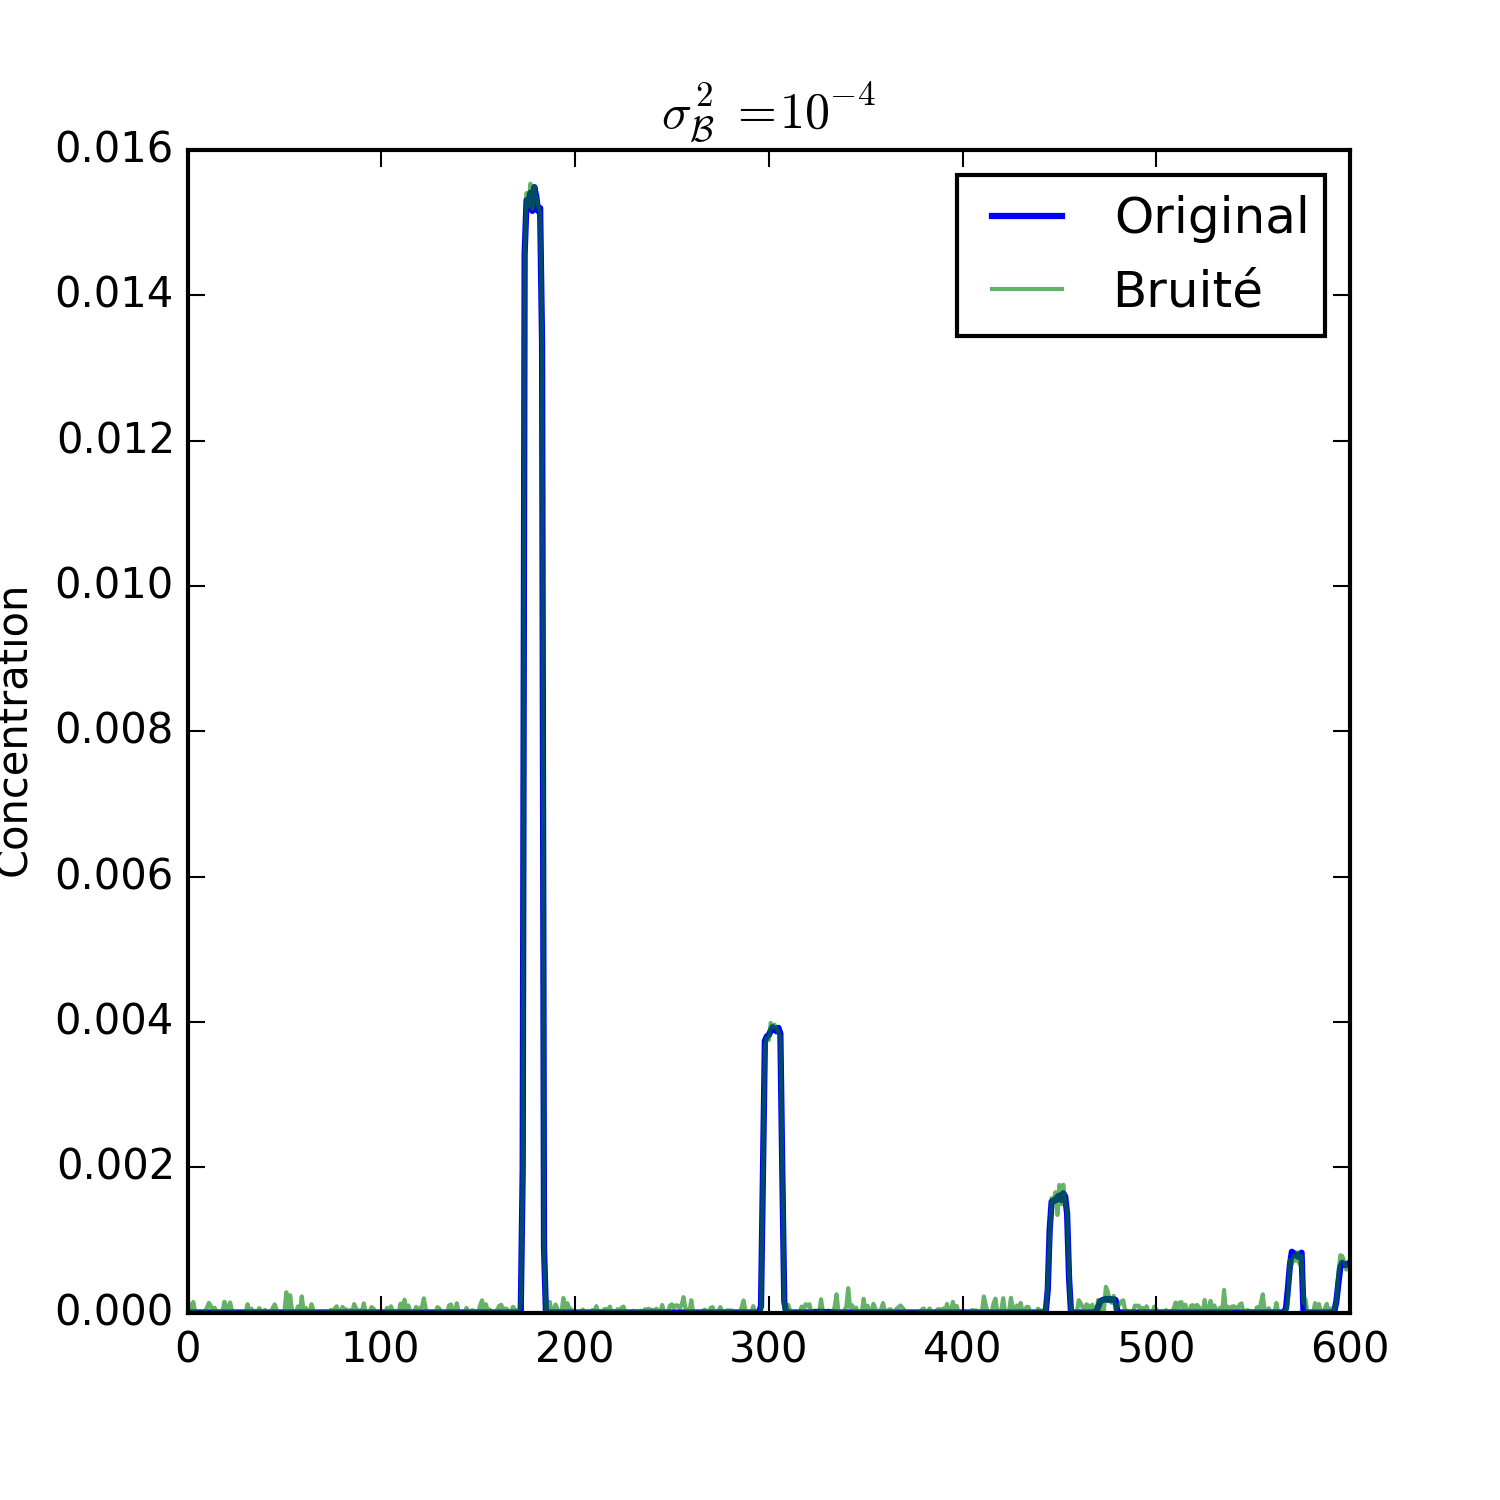
\includegraphics[width=1\textwidth]{25C_obs_noisy_1E4.png}
%		\caption{}
%		\label{}
%	\end{subfigure}%
%	\begin{subfigure}[t]{0.33\textwidth}
%		\centering
%		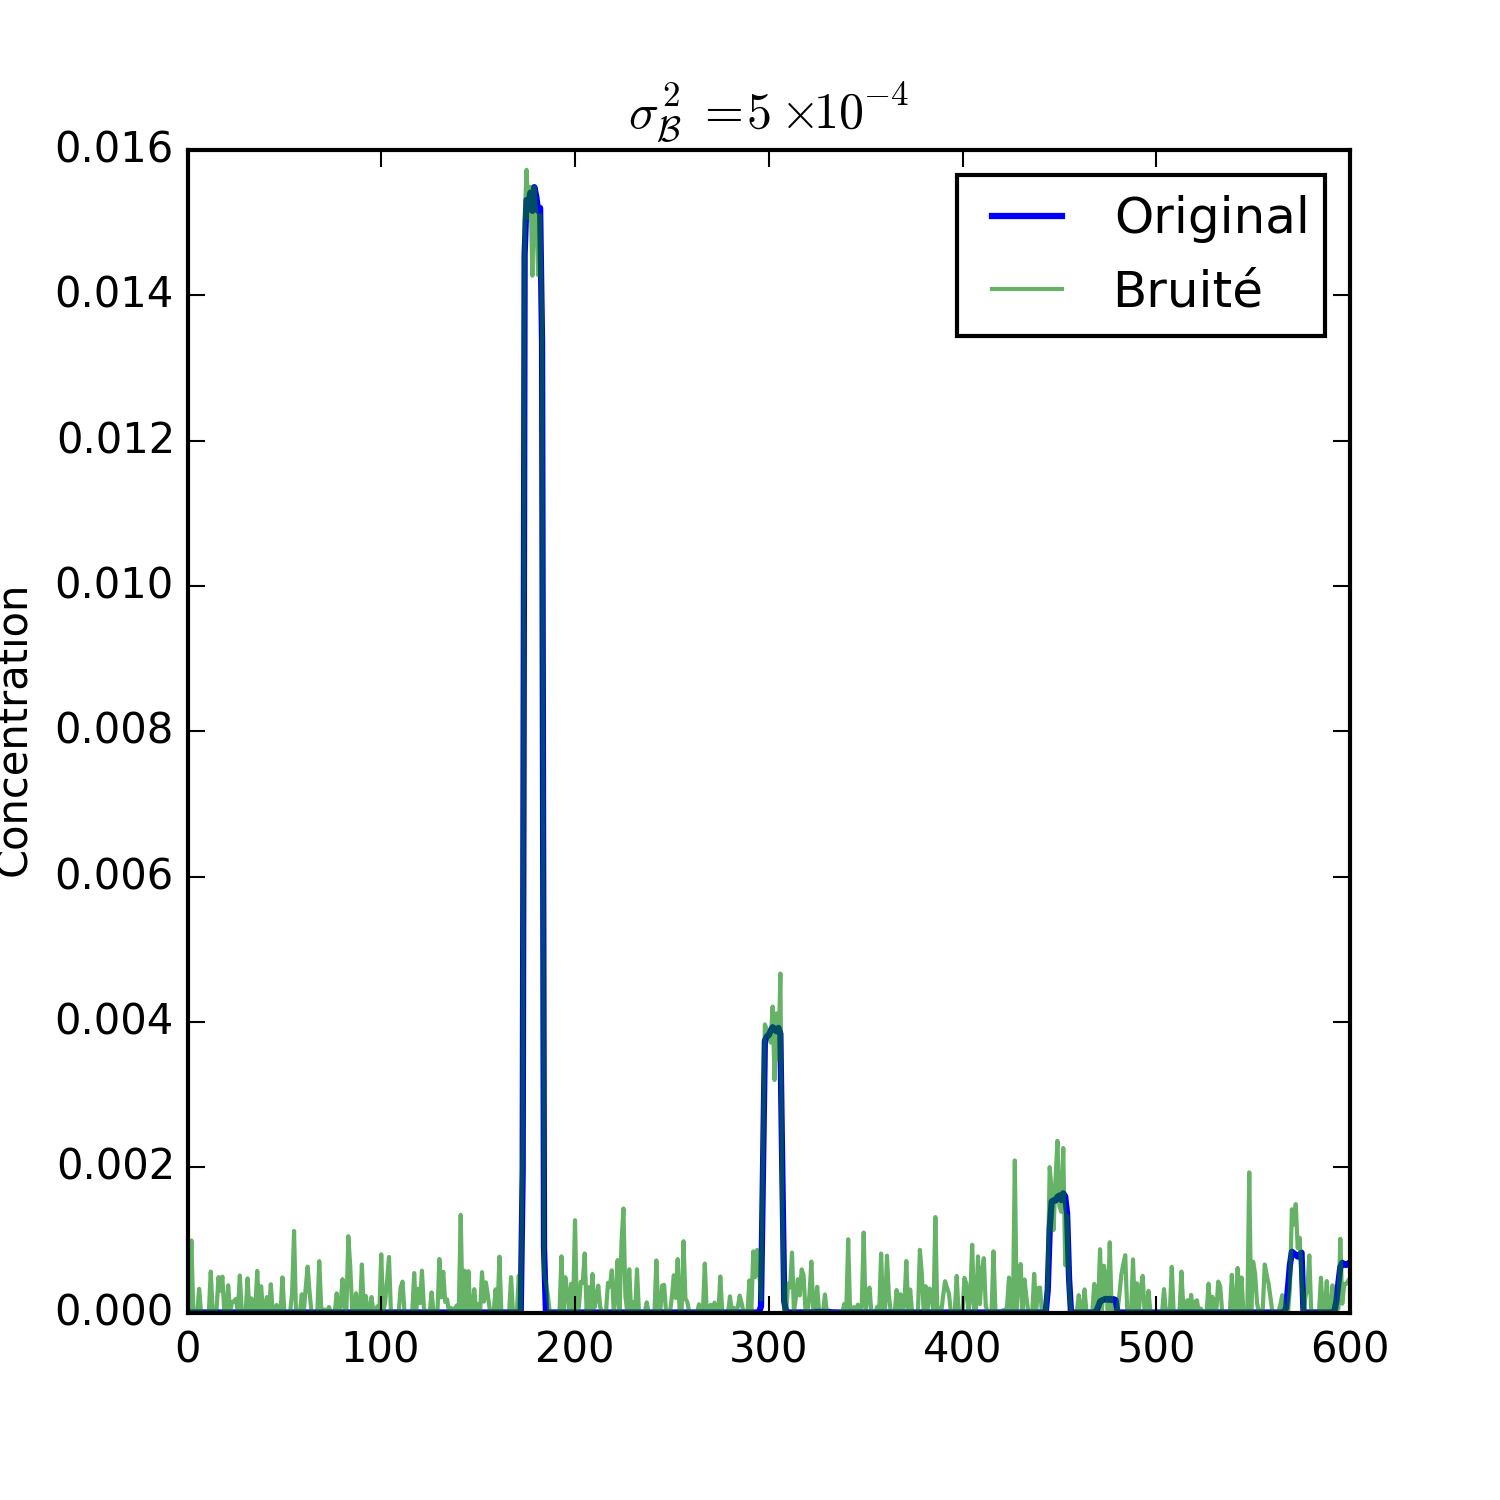
\includegraphics[width=1\textwidth]{25C_obs_noisy_5E4.png}
%		\caption{}
%		\label{}
%	\end{subfigure}%
%	\begin{subfigure}[t]{0.33\textwidth}
%		\centering
%		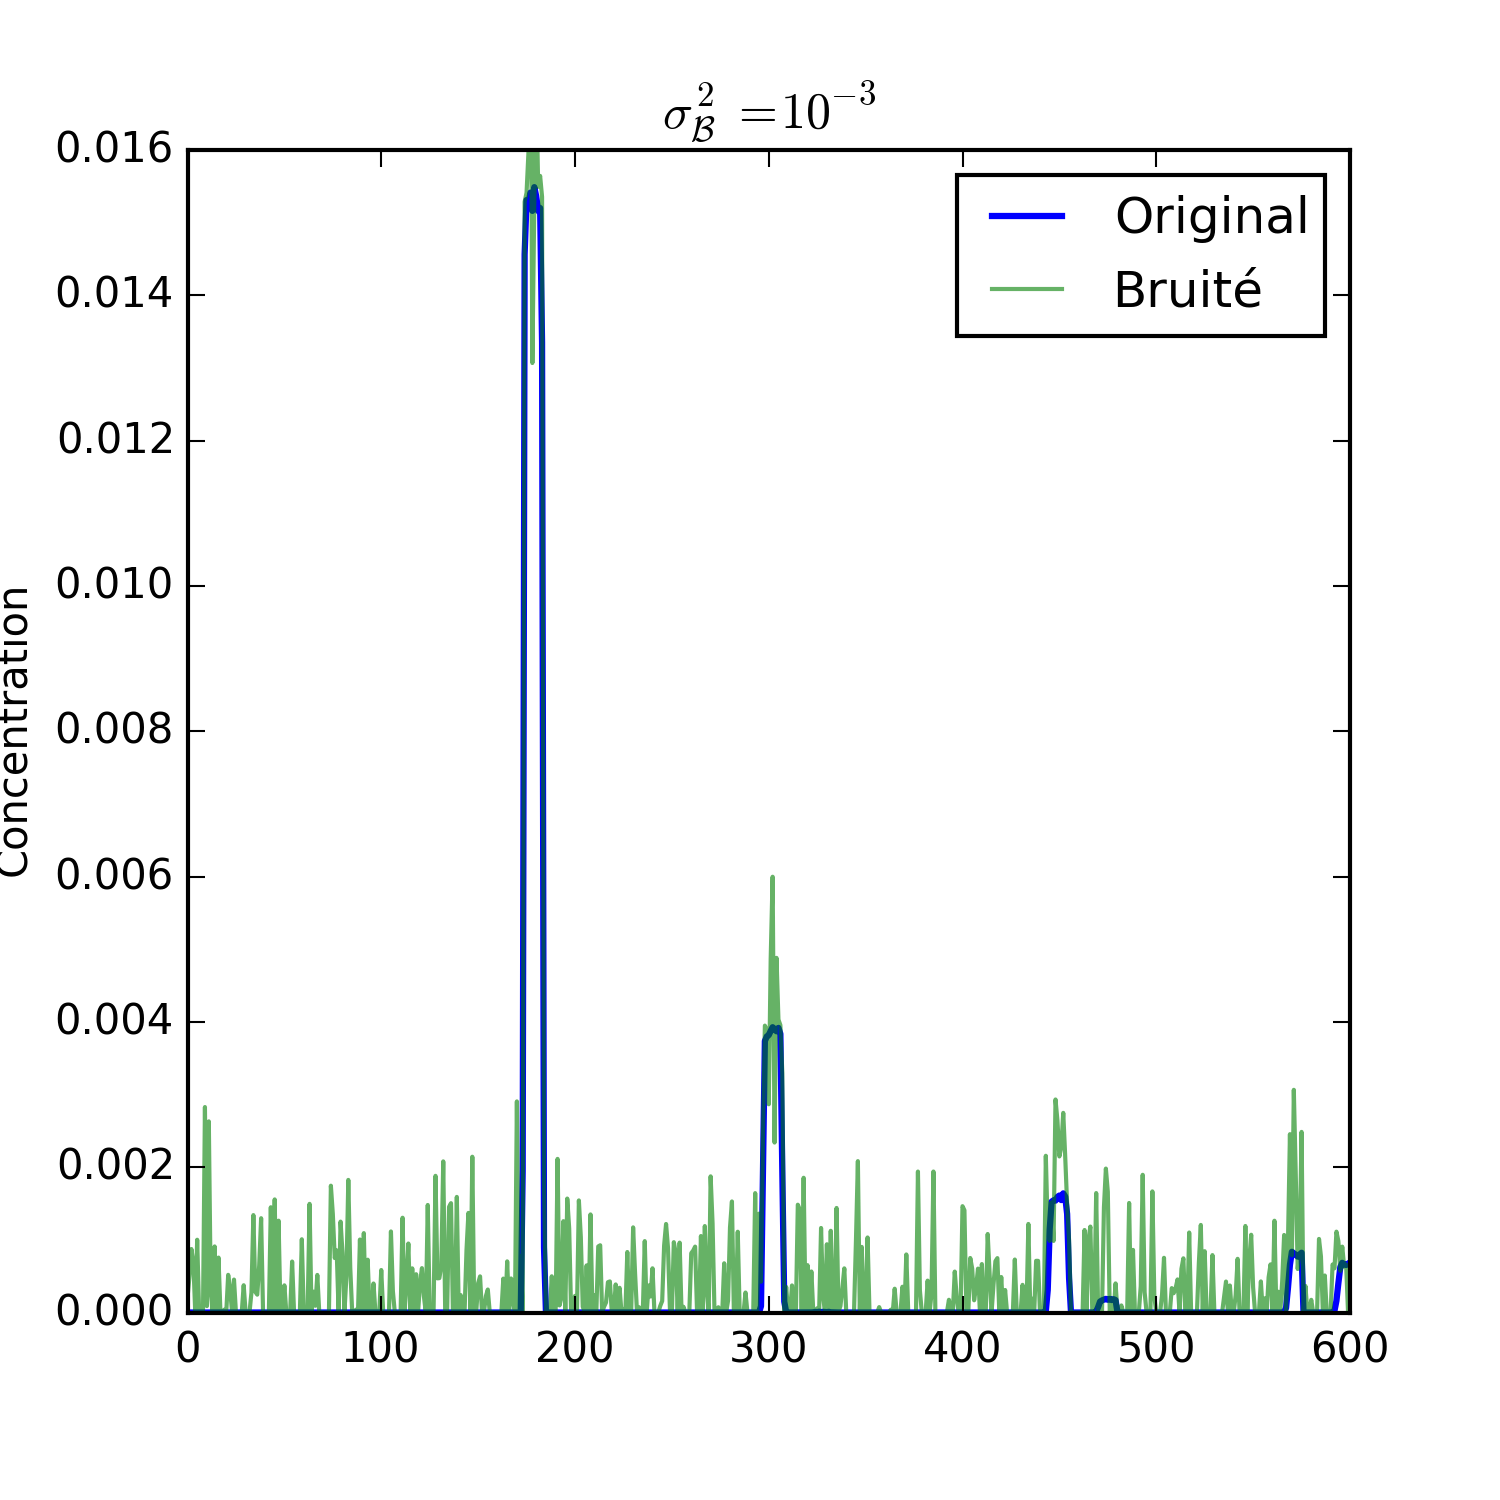
\includegraphics[width=1\textwidth]{25C_obs_noisy_1E3.png}
%		\caption{}
%		\label{}
%	\end{subfigure}%
%	\caption{Perturbation du vecteur d'observations $\VecObs$ par différentes intensités de bruit}
%	\label{fig_25C_obs_noisy}
%\end{figure}
%
%On  étudie ensuite les résultats d'estimation obtenus avec chacun de ces nouveaux vecteurs d'observations pour une variance $\varObs = 10^{-7}$ afin de comparer les différences de résultats avec et sans ajout de bruit.\\
%
%\todoin{1) Comparaison avec et sans bruit 2) Conclusion}

\subsection{Influence de la variance a priori du profil d'émission}

La variance a priori $\varQ$ peut être vue comme une hypothèse de départ sur l'amplitude possible des valeurs du profil d'émission. Son influence s'applique à la fois sur la qualité de la reconstruction de $\VecQSource$, mais également sur celle de la localisation de la source, car $\varQ$ intervient dans l'algorithme AMIS lors du calcul de la vraisemblance des particules. 

Pour cette analyse, on utilise le même procédé que pour l'étude de $\varObs$, en reprenant les paramètres du \textit{benchmark} et en exécutant 100 \textit{runs} de l'AMIS, les valeurs de $\varQ$ couvertes étant: $2\times 10^5, 7\times 10^5, 2\times 10^6, 7\times 10^6, 2\times 10^7$ et $7\times 10^7$.\\

Pour l'estimation de la position, on constate que plus la valeur de $\varQ$ considérée est grande, plus la source aura tendance à être estimée en amont  par rapport à la direction du vent. En effet, pour la même position potentielle de la source, des valeurs plus élevées pour les quantités de polluant rejetées impliquent des mesures de concentration plus importantes aux capteurs: l'algorithme va donc ajuster cette position en remontant l'axe du vent pour avoir une meilleure vraisemblance par rapport aux observations. Ce phénomène de décalage spatial est bien visible sur la figure \ref{fig_25C_varQ_boxplots}, où les \textit{boxplots} des estimations ponctuelles sont tracées pour chacune des valeurs de $\varQ$ testées.

\begin{figure}[h!]
	\centering
         	\begin{subfigure}[t]{0.5\textwidth}
         		\centering
         		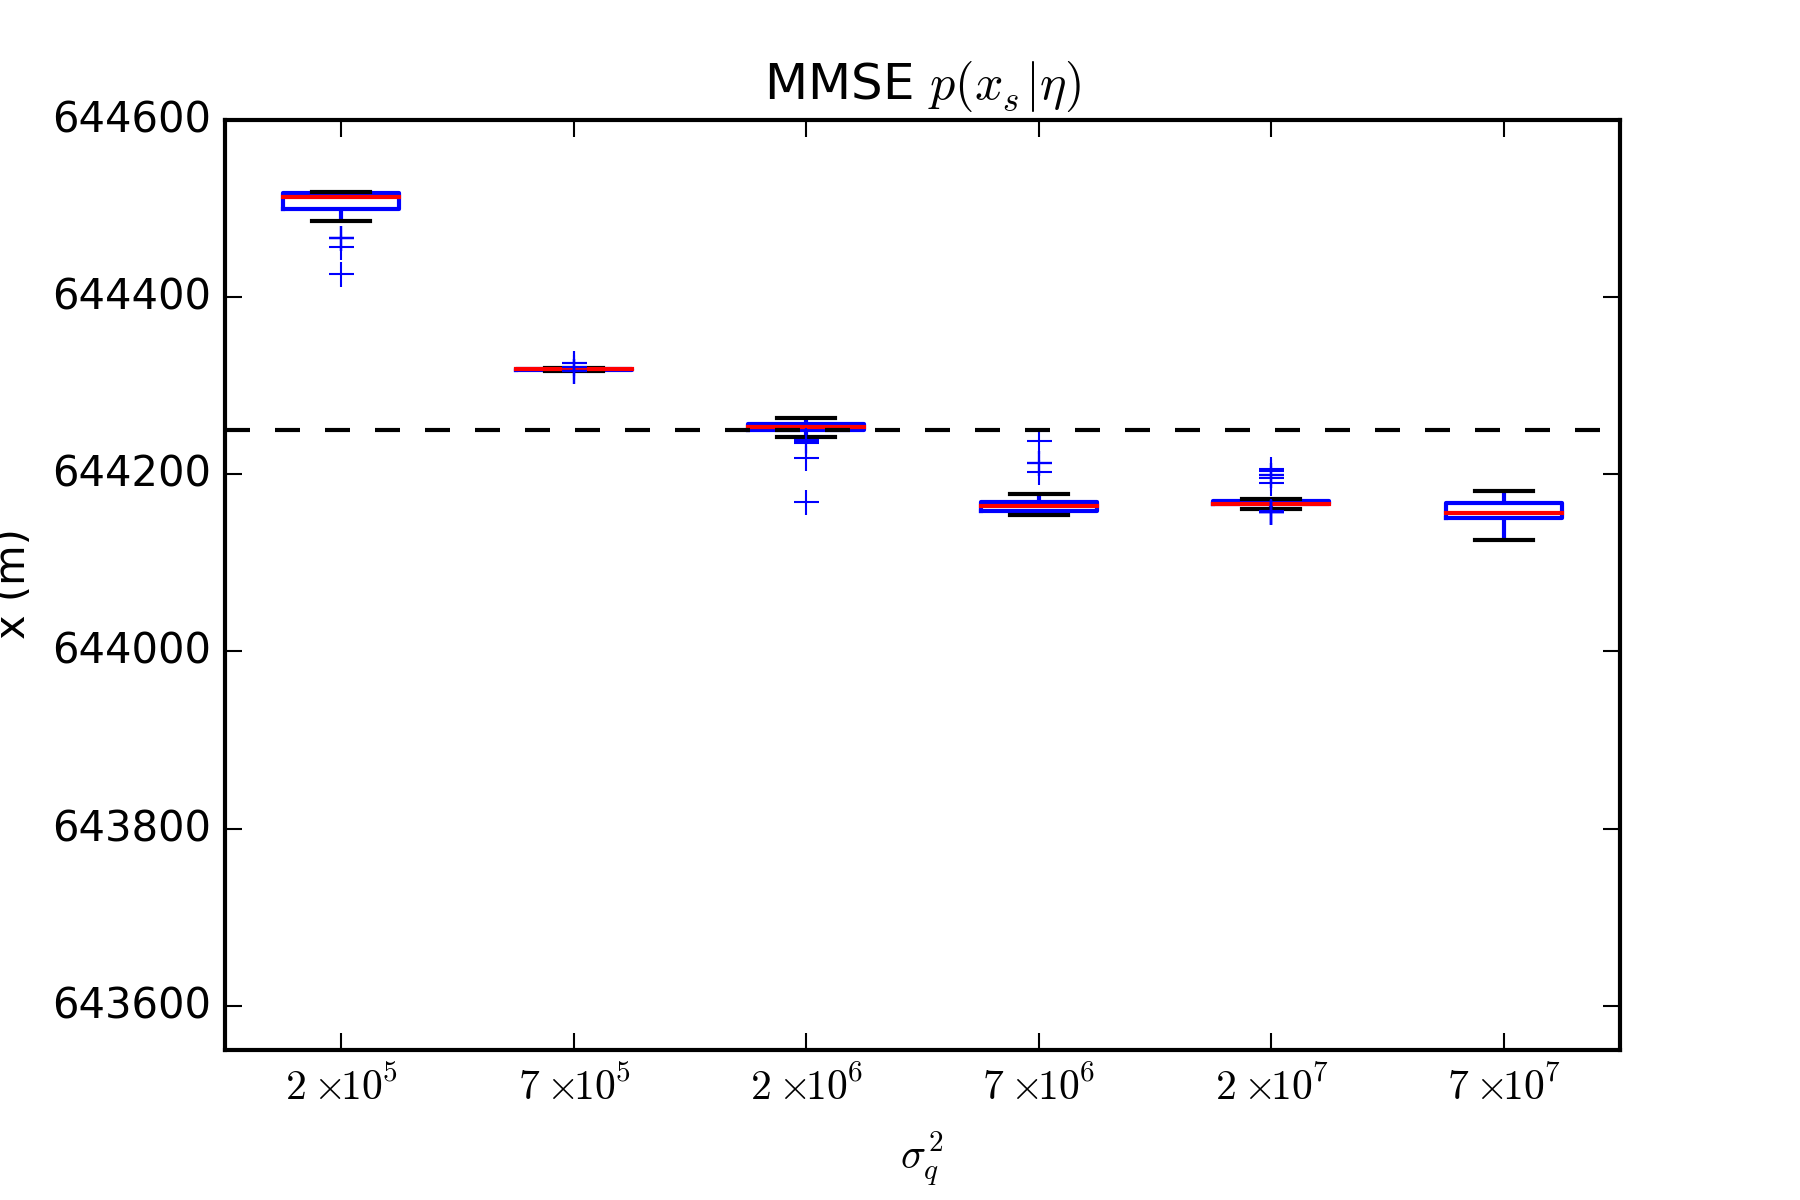
\includegraphics[width=1\textwidth]{25C_varQ_boxplot_x.png}
         		\caption{}
         		\label{varQ_boxplot_x}
         	\end{subfigure}%         	
         \begin{subfigure}[t]{0.5\textwidth}
         	\centering
         	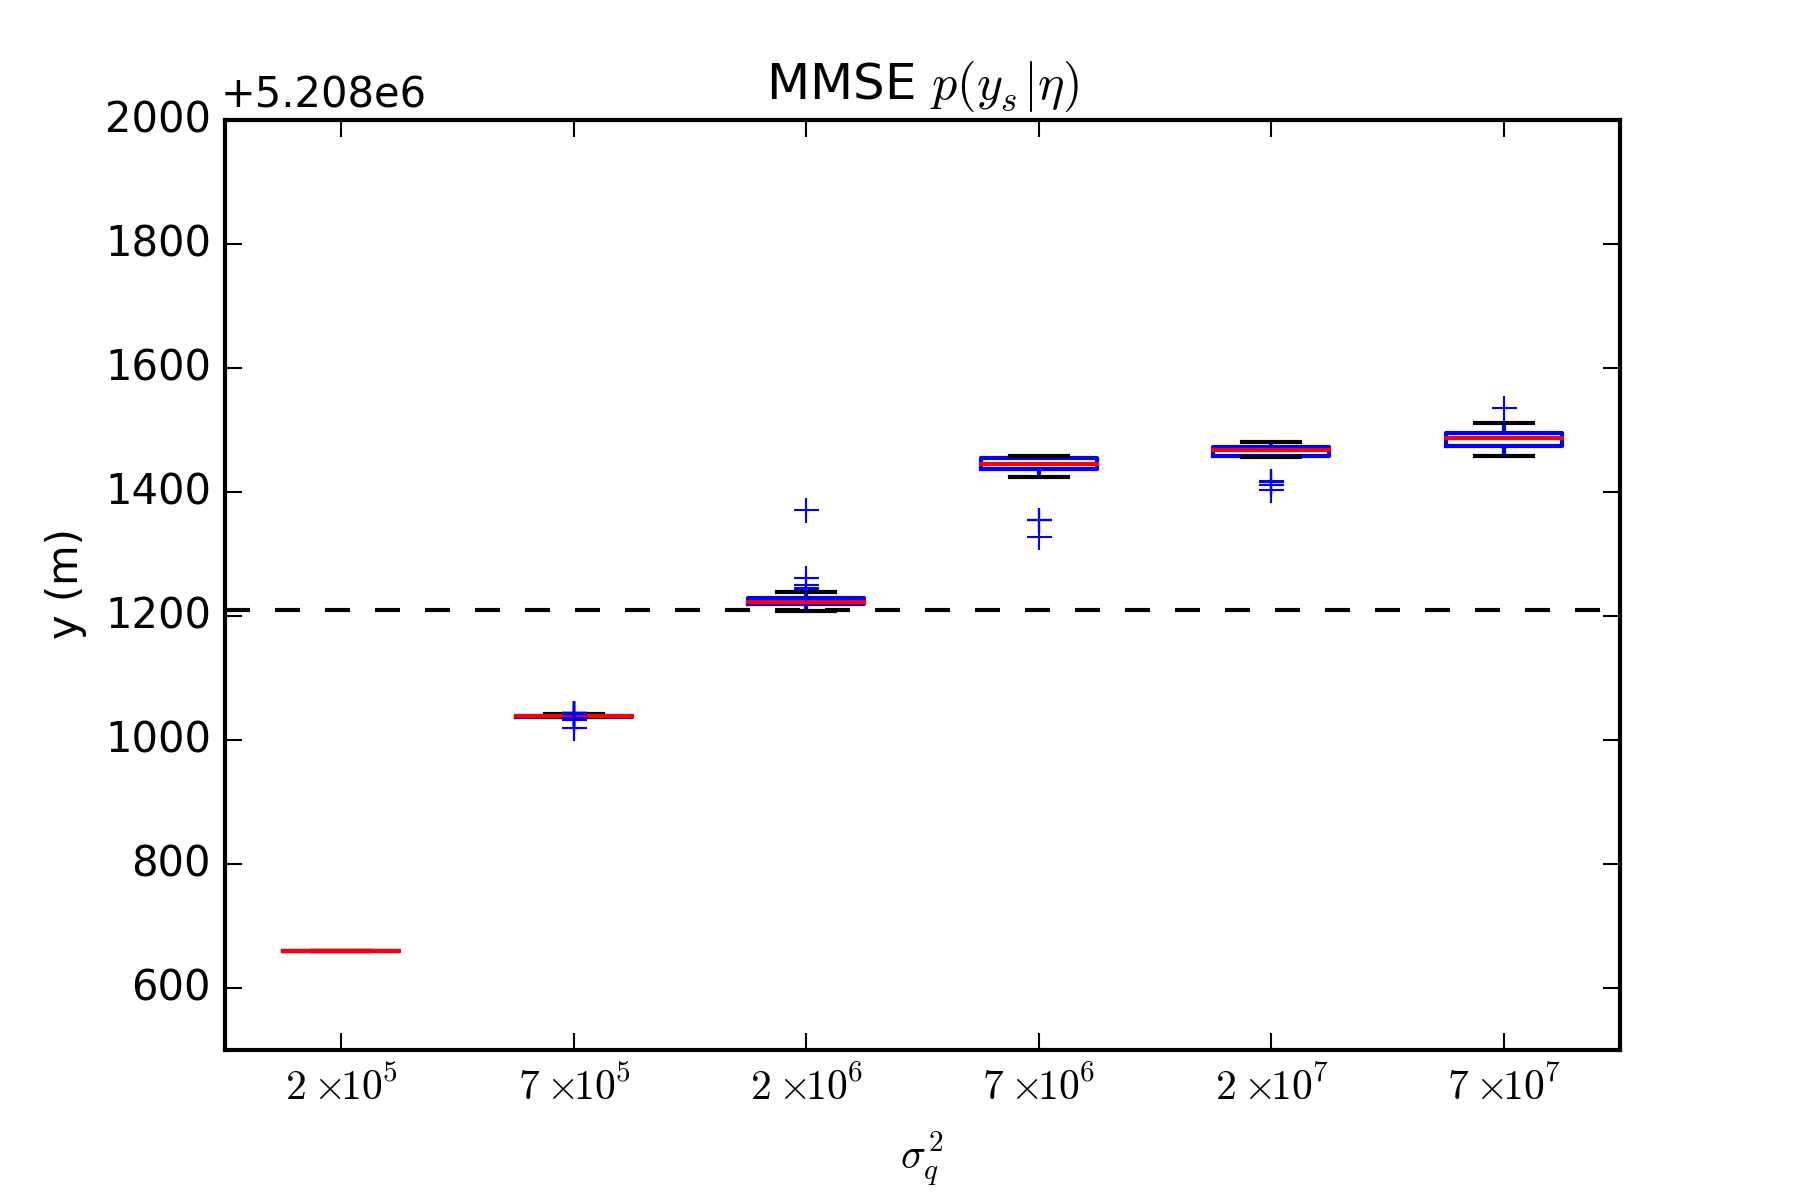
\includegraphics[width=1\textwidth]{25C_varQ_boxplot_y.png}
         	\caption{}
         	\label{varQ_boxplot_y}
         \end{subfigure}%
         \caption{\textit{Boxplots} des estimations par MMSE de la position de la source sur 100 runs, comparaison avec les valeurs réelles (en pointillés noirs)}
         \label{fig_25C_varQ_boxplots}
	
\end{figure}

La meilleure estimation du profil d'émission est obtenue pour $\varQ=2\times 10^6$ (voir figure \ref{fig_25C_analyse_varq_q} de l'Annexe A), ce qui coïncide avec la meilleure position estimée dans la figure \ref{fig_25C_varQ_boxplots}. Pour des valeurs plus faibles de $\varQ$ le débit est sous-estimé, à l'inverse pour des valeurs plus élevées le débit est surestimé. On peut résumer ce comportement grâce aux courbes d'erreur de la figure \ref{fig_25C_varq_erreurs}.

         \begin{figure}[h!]
         	\centering
         	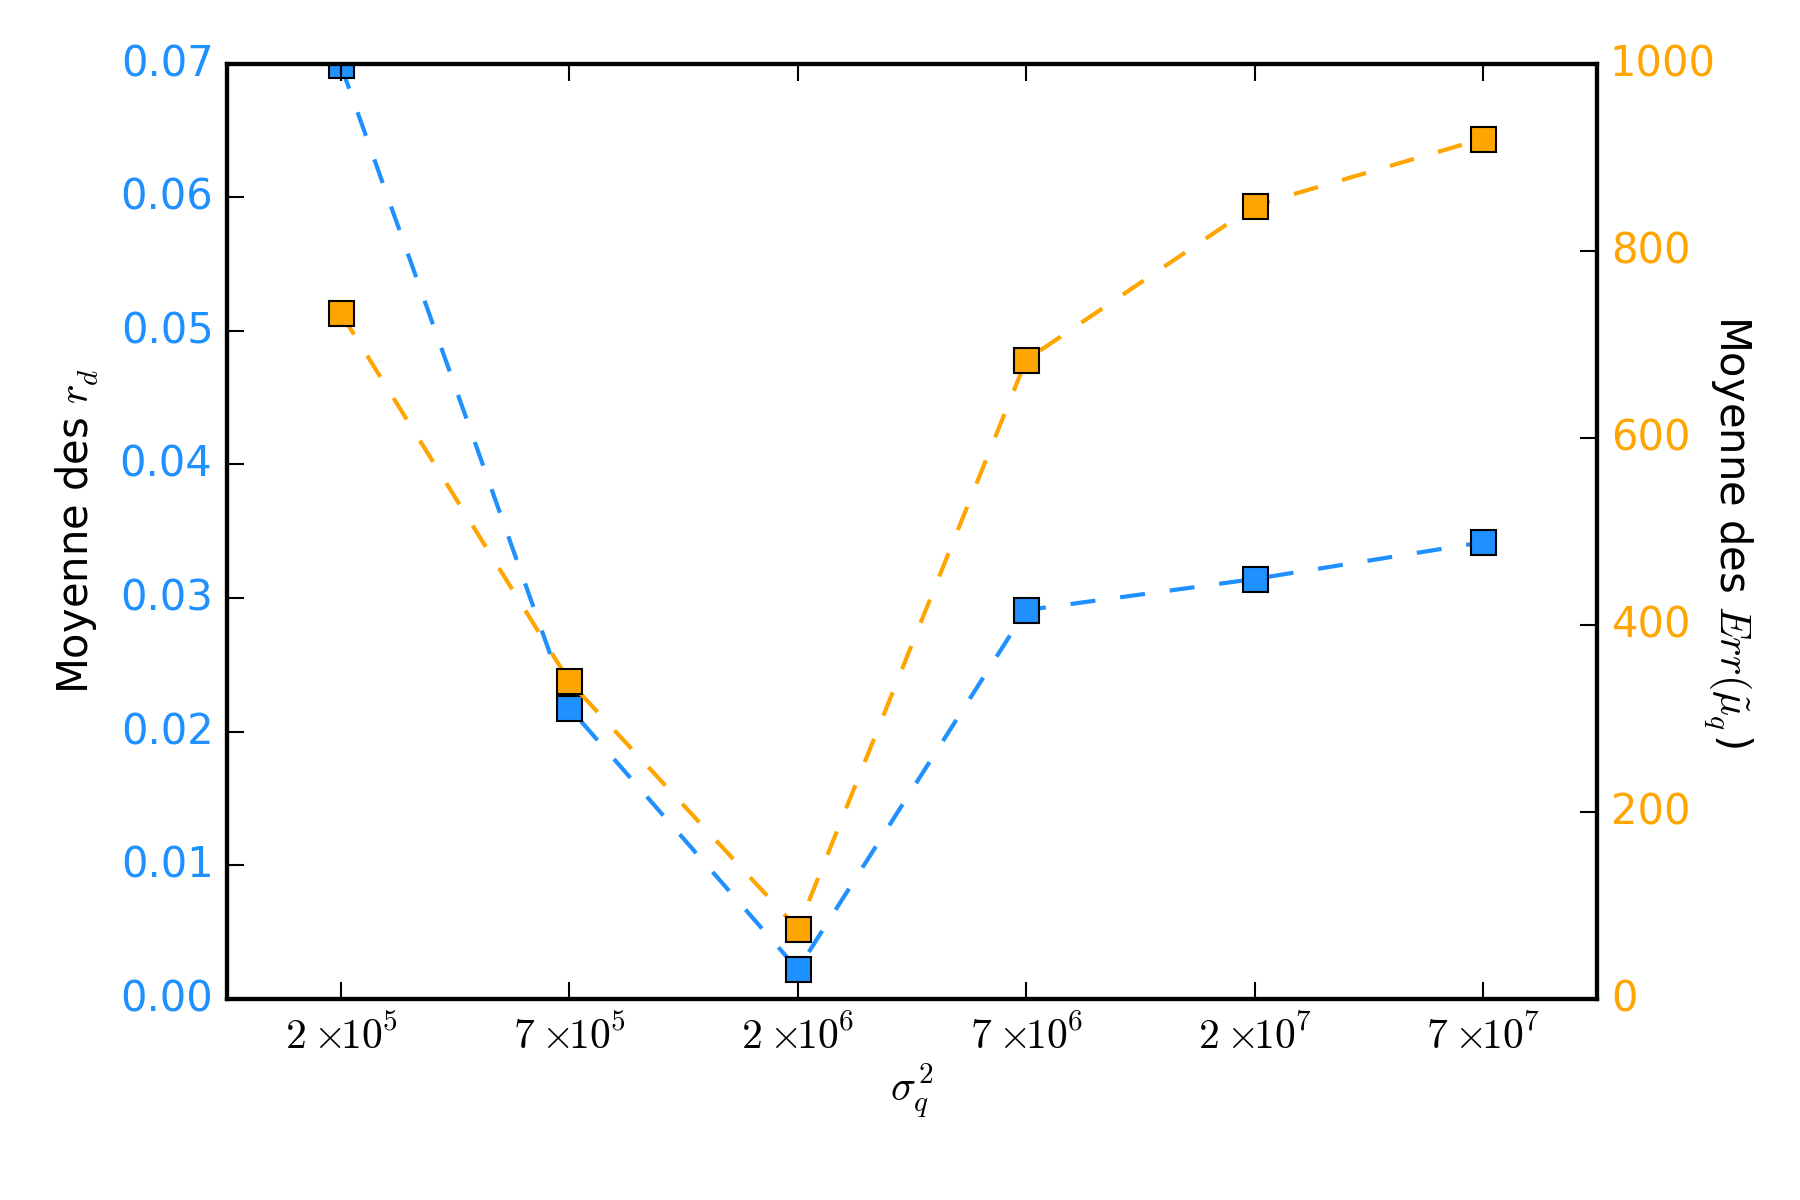
\includegraphics[width=0.8\textwidth]{25C_varQ_errors.png}
         	\caption{Courbes d'erreur pour l'analyse paramétrique de $\varQ$}
         	\label{fig_25C_varq_erreurs}
         \end{figure}

\subsection{Influence de la densité du réseau de capteurs}

Le nombre et de la répartition des capteurs constitue un facteur important: 

\begin{itemize}
	\item du point de vue théorique, son étude permet de mieux comprendre le comportement de l'algorithme d'estimation et quantifier son importance par rapport aux autres variables,
	\item en pratique, l'analyse des résultats d'estimation en fonction de la configuration des capteurs permet un meilleur dimensionnement du réseau de mesure.\\
\end{itemize}

\subsubsection{Impact du capteur R8}

Dans un premier temps, nous nous intéressons à l'influence du capteur R8, qui est le récepteur le plus proche de la source à mesurer des concentrations non-nulles. Pour cela, nous le retirons du réseau, et nous effectuons l'opération d'estimation du terme source avec les observations issues des 24 capteurs restants, en suivant les paramètres du \textit{benchmark}. En pratique, cela reviendrait par exemple à simuler la panne du capteur R8 durant la fenêtre temporelle d'observation.\\


\begin{figure}[h!]
	\centering
	\begin{subfigure}[t]{0.5\textwidth}
		\centering
		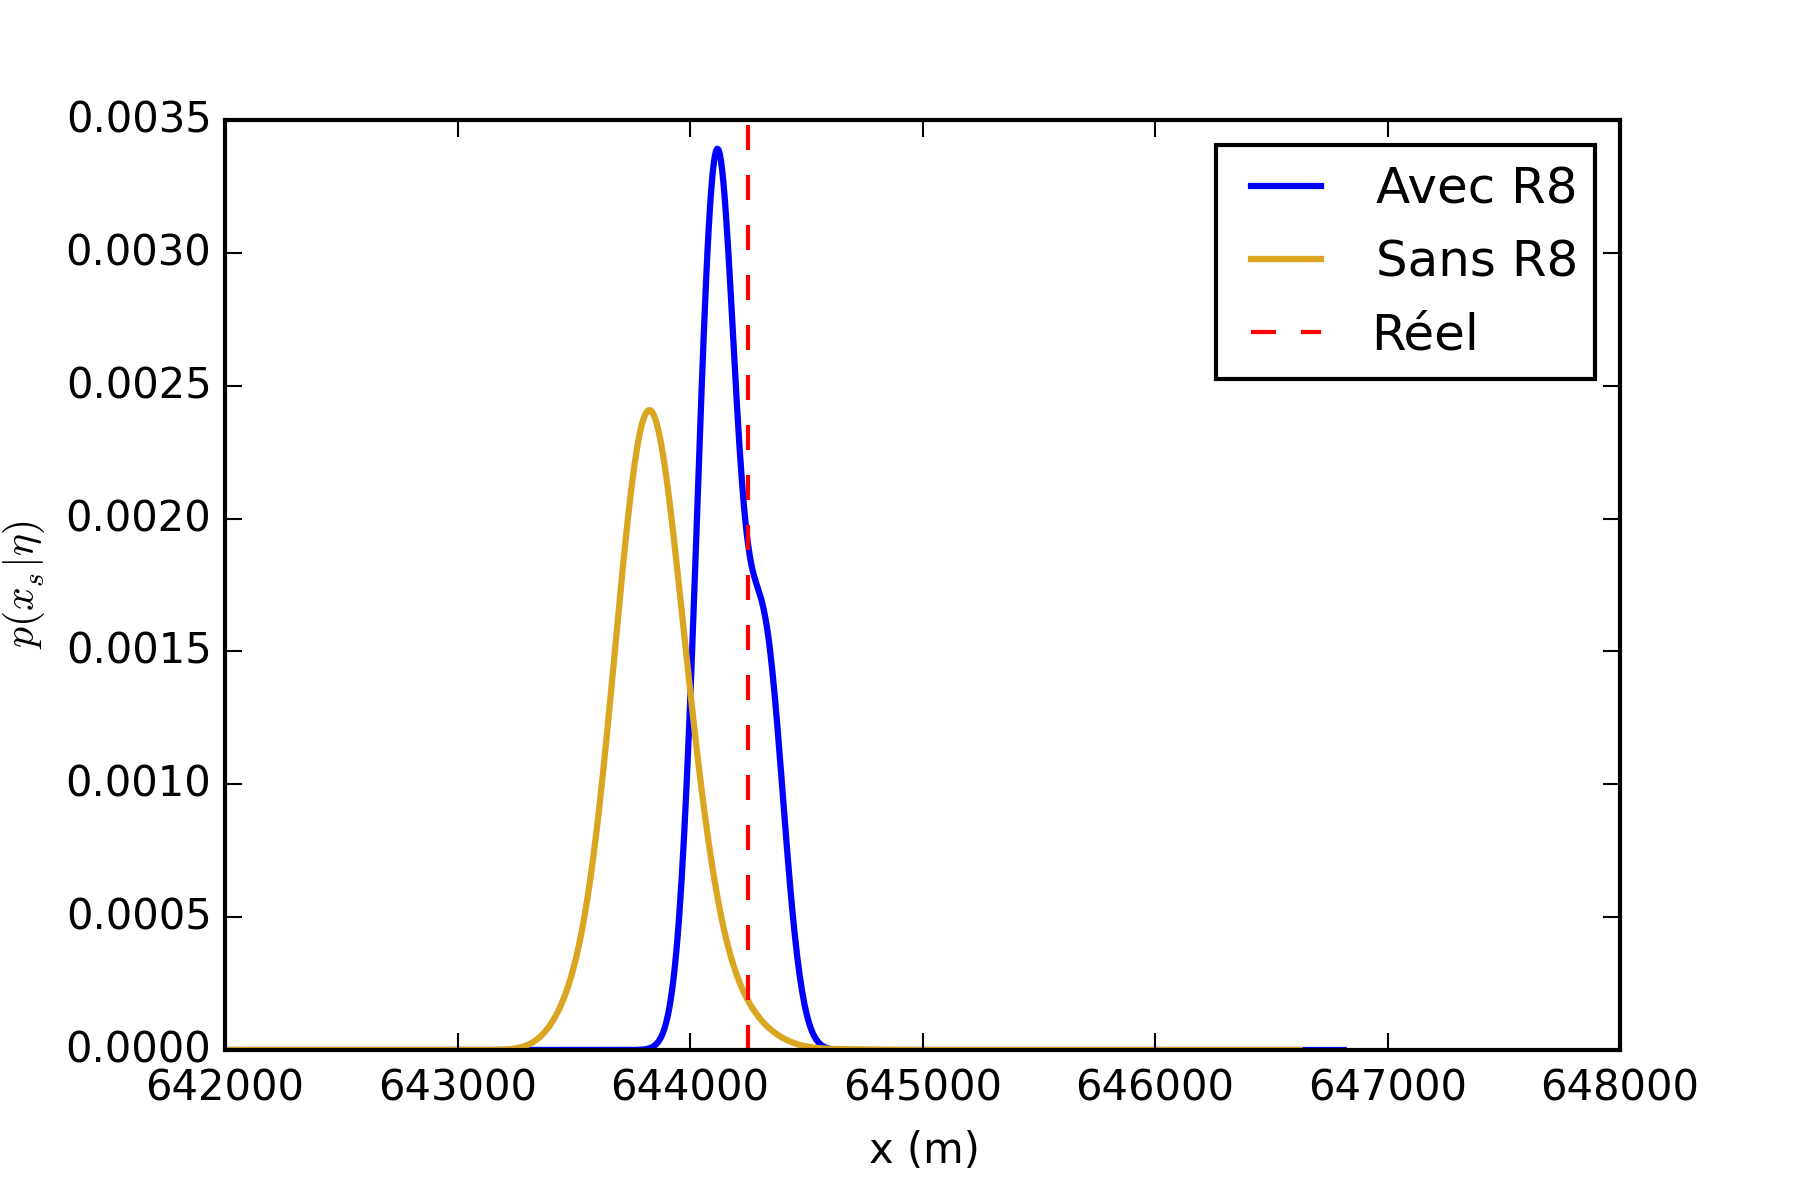
\includegraphics[width=1\textwidth]{R8_kde_x_compare.png}
		\caption{Position en $x$}
		\label{R8_x}
	\end{subfigure}%
	\begin{subfigure}[t]{0.5\textwidth}
		\centering
		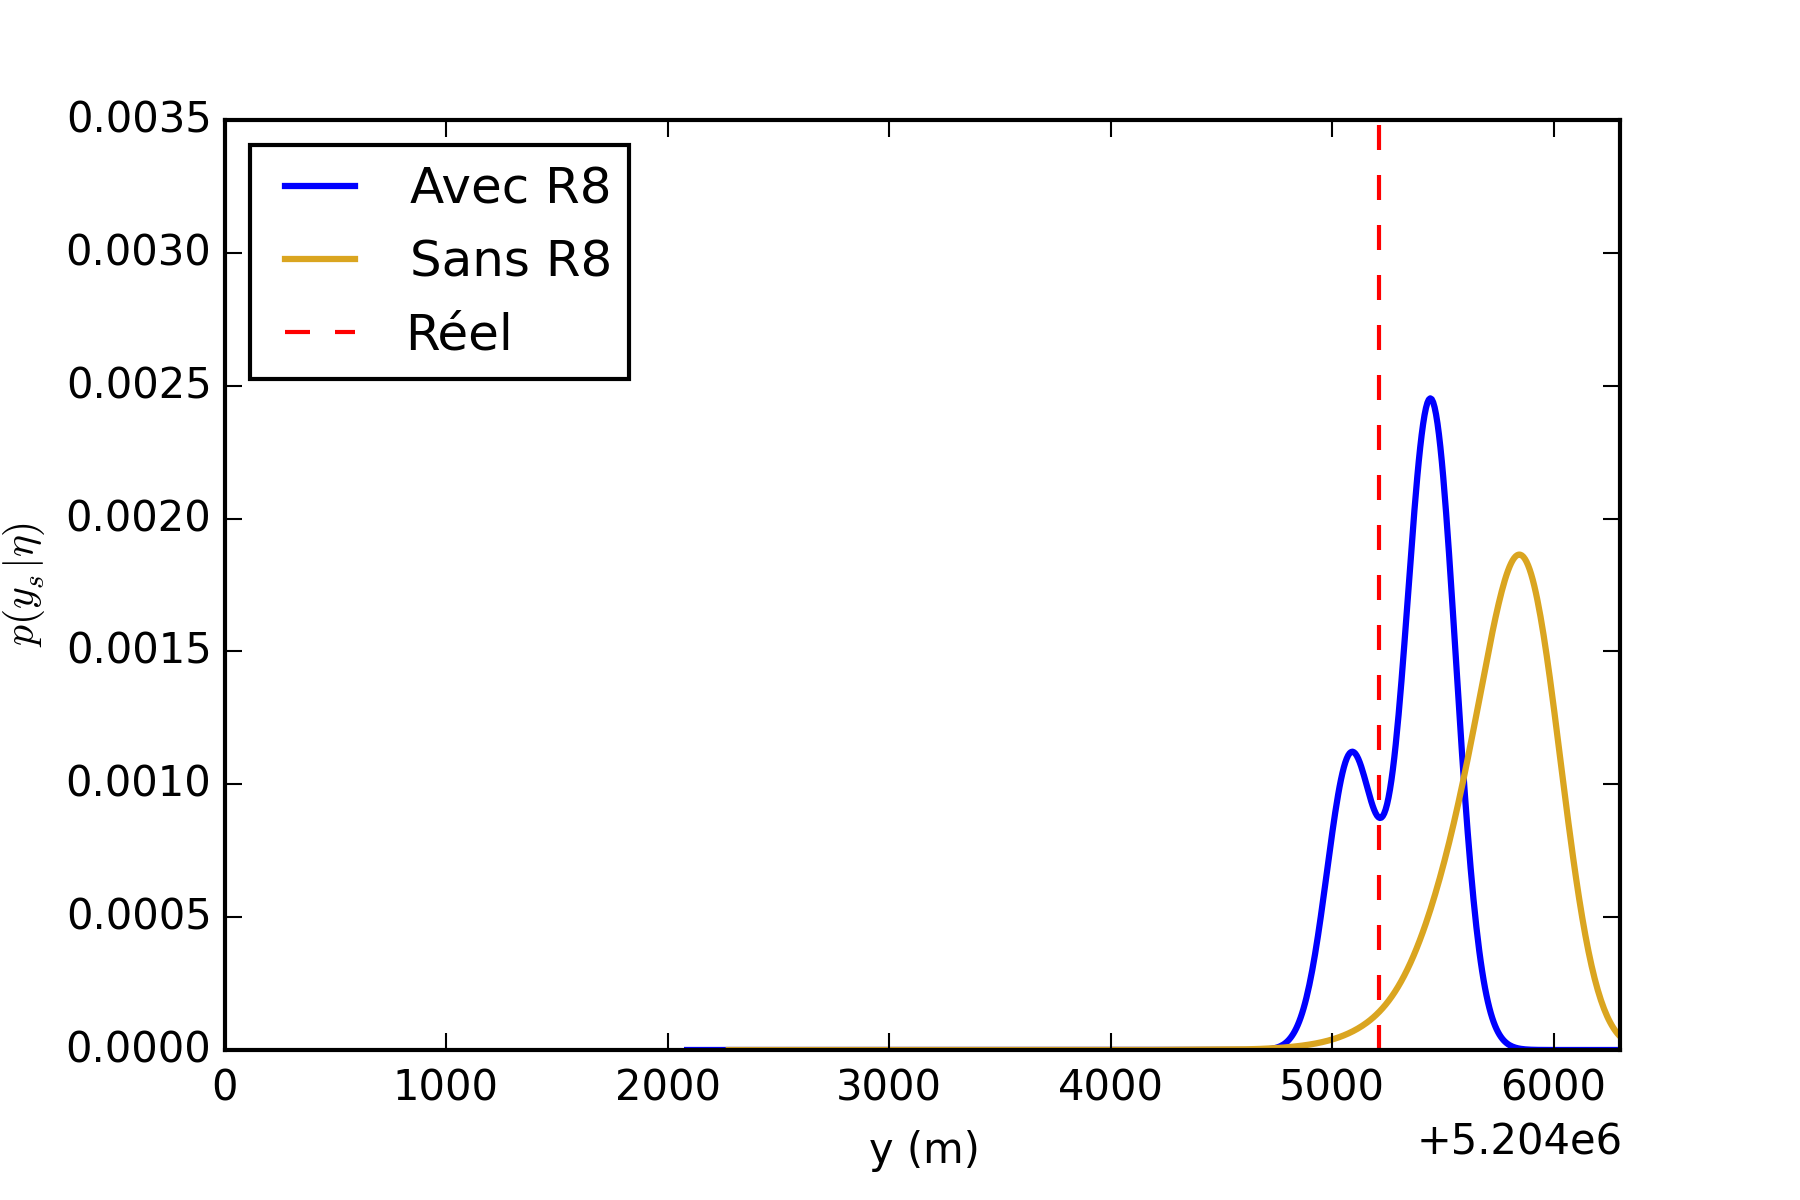
\includegraphics[width=1\textwidth]{R8_kde_y_compare.png}
		\caption{Position en $y$}
		\label{R8_y}
	\end{subfigure}
	\begin{subfigure}[t]{0.65\textwidth}
		\centering
		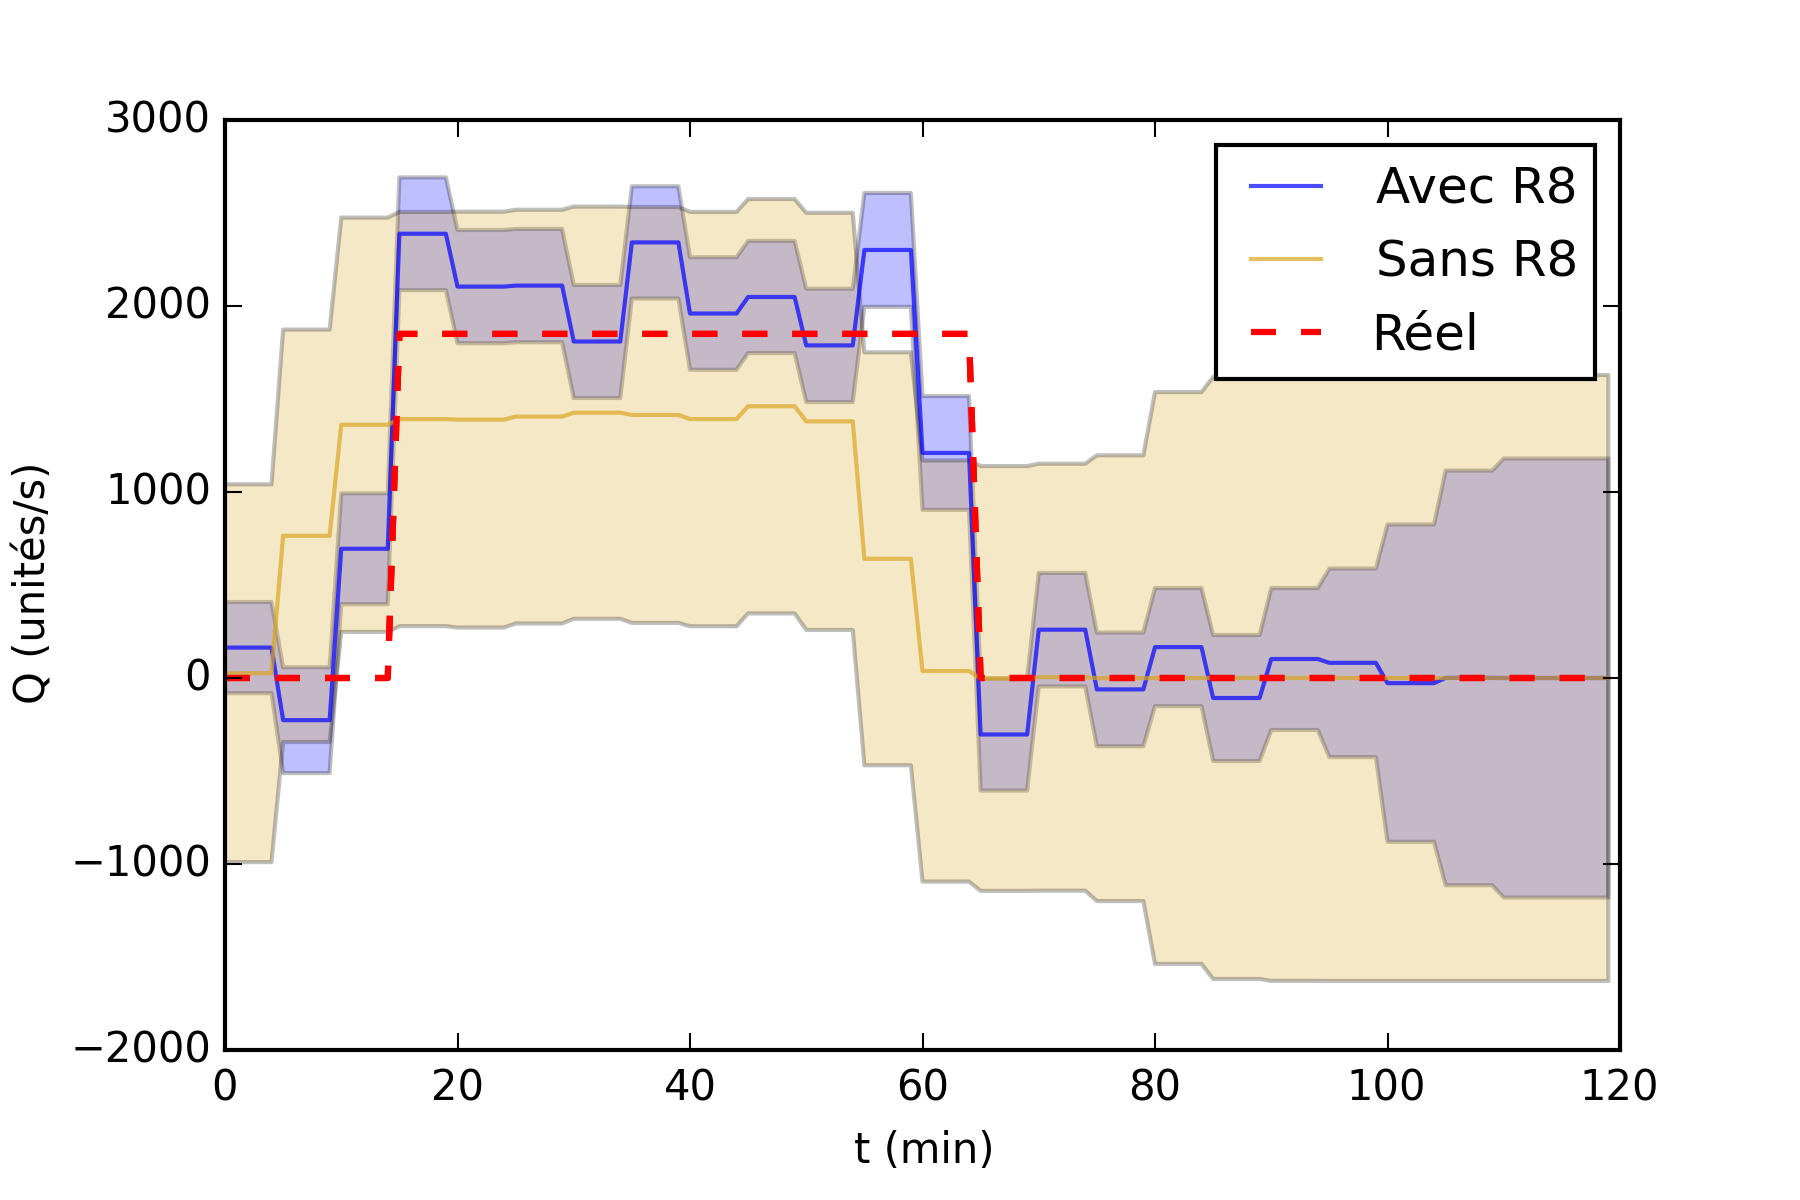
\includegraphics[width=1\textwidth]{R8_q_est_compare.png}
		\caption{Profil d'émission avec intervalle de confiance à  $\pm 2 \tilde{\sigma}_q^2$}
		\label{R8_q}
	\end{subfigure} 
	\caption{Résultats d'un \textit{run} de l'algorithme d'estimation sans (jaune) et avec (bleu) le capteur R8}
	\label{fig_R8_compare}
\end{figure}

A paramètres identiques, la source est vue plus en amont sur l'axe du vent par rapport à sa position réelle (figures \ref{R8_x} et \ref{R8_y}). De plus, sans le capteur R8, le débit est relativement sous-estimé par rapport aux valeurs attendues, et le rejet reconstitué commence et s'achève plus tôt que prévu (figure \ref{R8_q}). On observe ainsi que les mesures fournies par le capteur R8 apportent une information non-négligeable permettant d'accroître la précision de l'estimation, à la fois sur les aspects spatiaux, temporels, et de quantité émise. 

\subsubsection{Impact d'un réseau réduit}

On a vu que le rôle individuel des capteurs peut être important pour pouvoir reconstruire correctement un terme source. Nous cherchons ici à savoir comment varie la qualité de cette reconstruction si l'ensemble du réseau est modifié.

On réduit ainsi la taille de notre réseau à 9 capteurs (figure \ref{fig_reseaux_25_9}), répartis de façon homogène sur le domaine. Cela permet de simuler une situation où le nombre d'instruments de mesure des concentrations est moindre (par exemple, dans le cas où les capteurs sont coûteux à acheter et à déployer), et également d'apprécier le comportement de l'algorithme d'estimation lorsque la représentativité spatiale des mesures est limitée. Les paramètres d'entrée de l'algorithme d'estimation sont toujours ceux du \textit{benchmark}.\\

\begin{figure}[h!]
	\centering
	\begin{subfigure}[t]{0.5\textwidth}
		\centering
		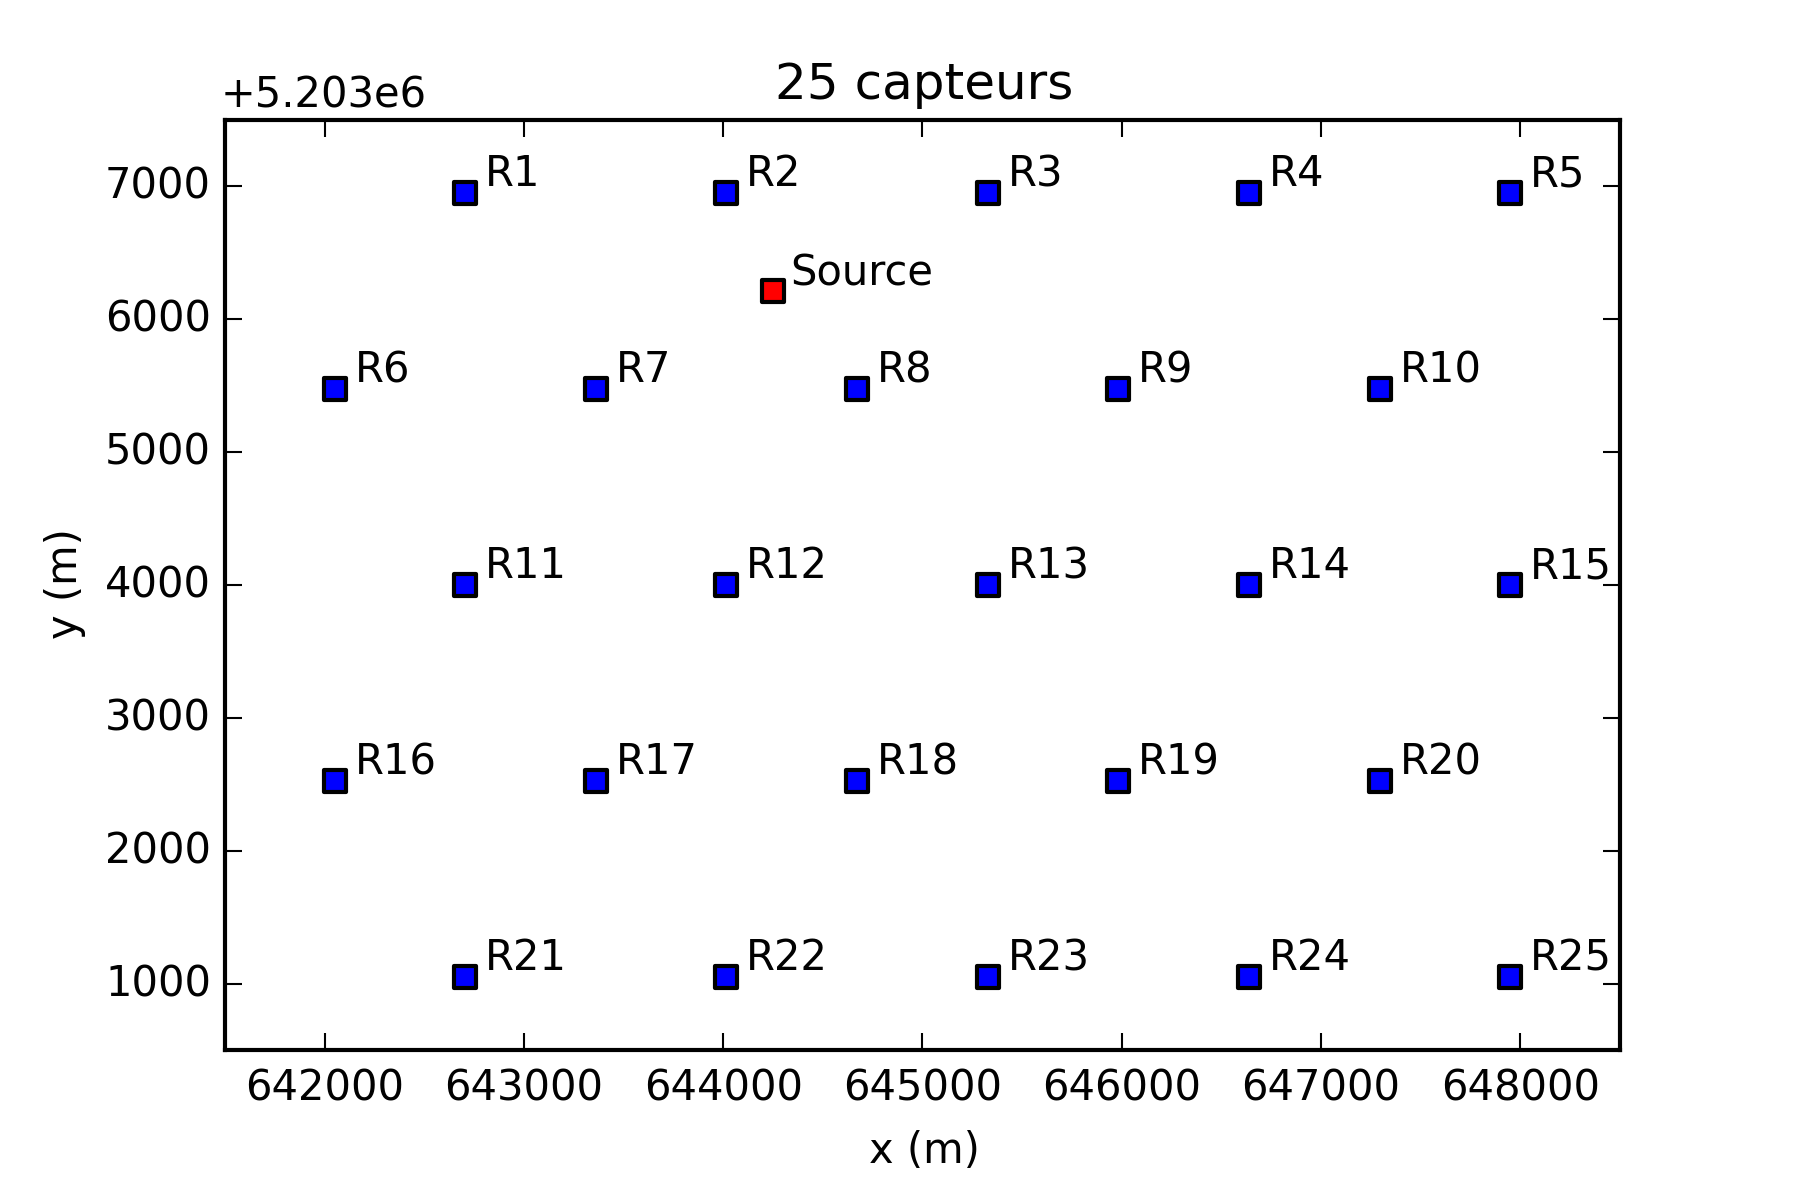
\includegraphics[width=1\textwidth]{reseau_25C.png}
		\caption{}
		\label{reseau_25C}
	\end{subfigure}%
	\begin{subfigure}[t]{0.5\textwidth}
		\centering
		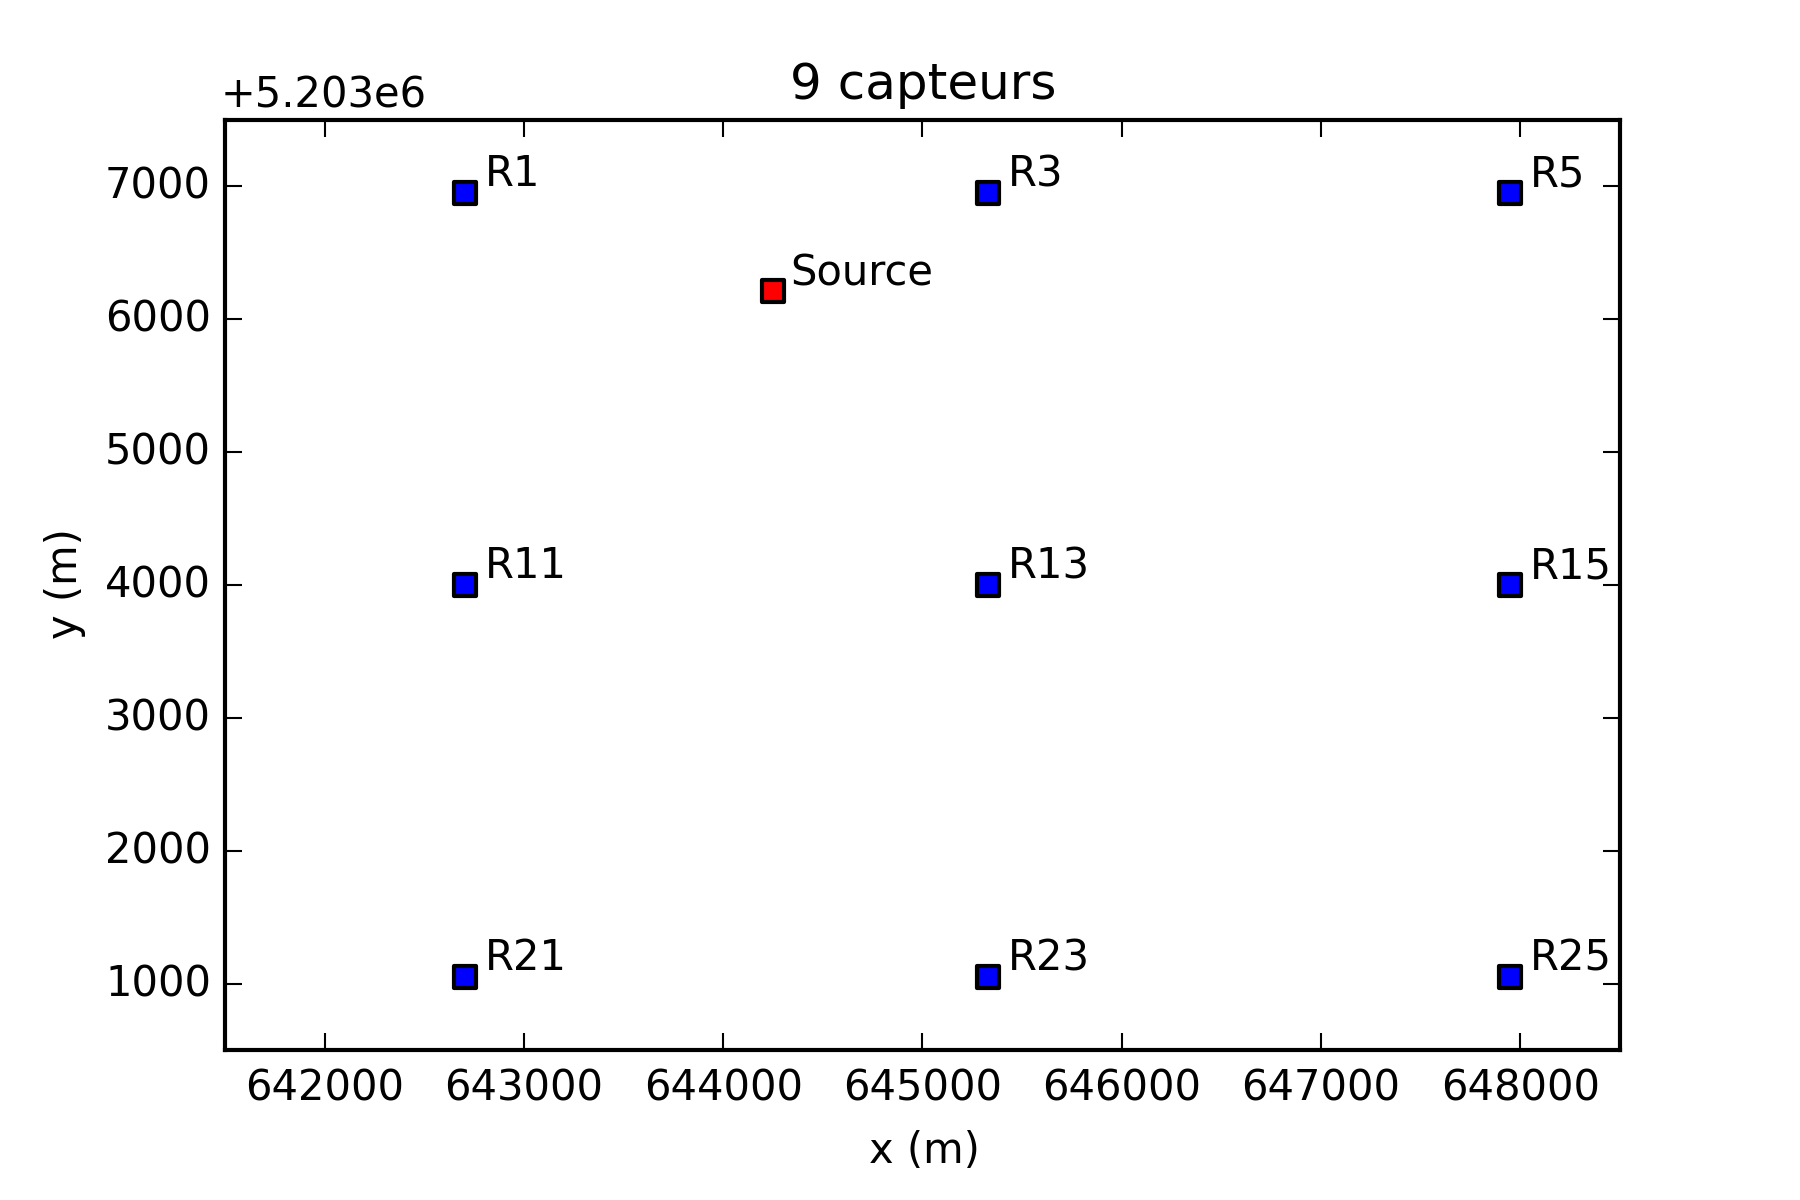
\includegraphics[width=1\textwidth]{reseau_9C.png}
		\caption{}
		\label{reseau_9C}
	\end{subfigure}
	\caption{Réduction de la densité du réseau de capteurs: passage de 25 (gauche) à 9 (droite) capteurs}
	\label{fig_reseaux_25_9}
\end{figure}


\begin{figure}[h!]
	\centering
	\begin{subfigure}[t]{0.5\textwidth}
		\centering
		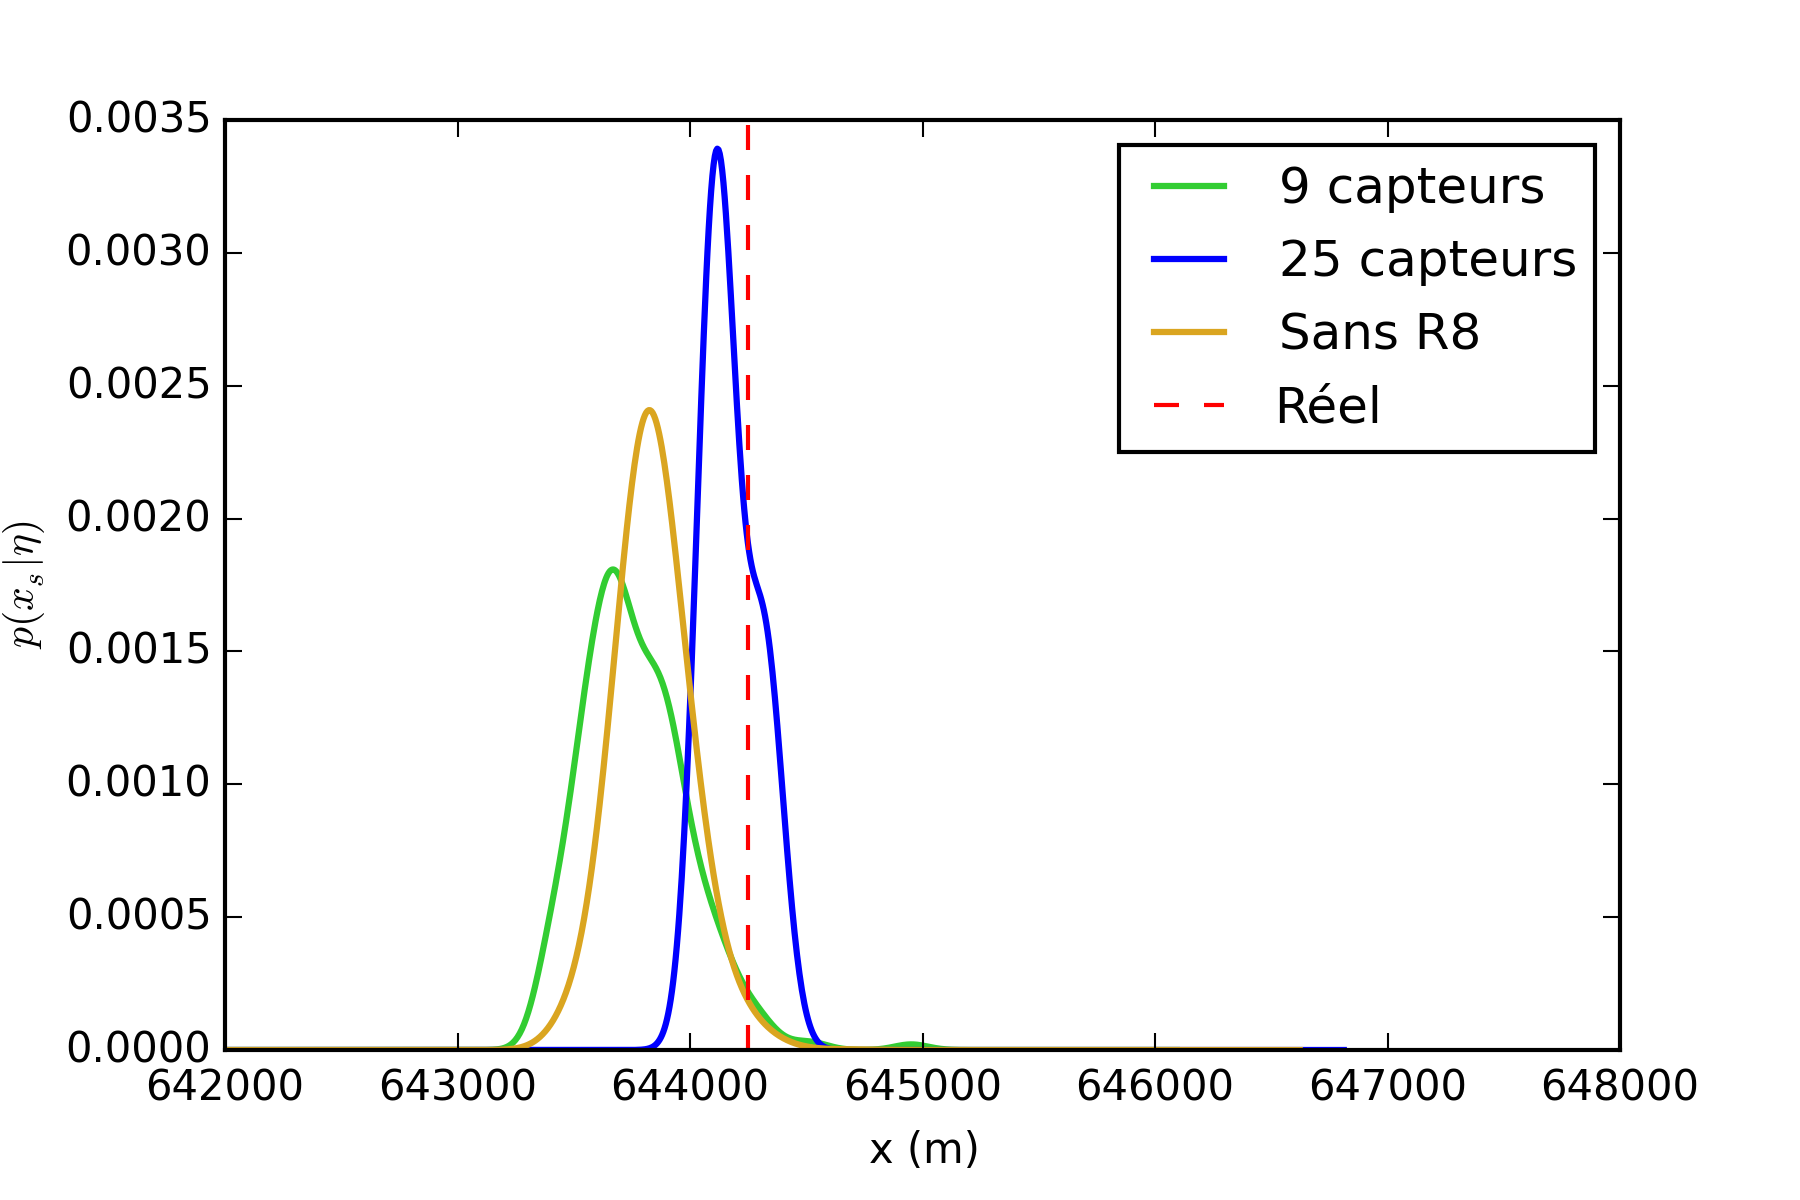
\includegraphics[width=1\textwidth]{kde_x_compare_all.png}
		\caption{}
		\label{kde_x_all}
	\end{subfigure}%
	\begin{subfigure}[t]{0.5\textwidth}
		\centering
		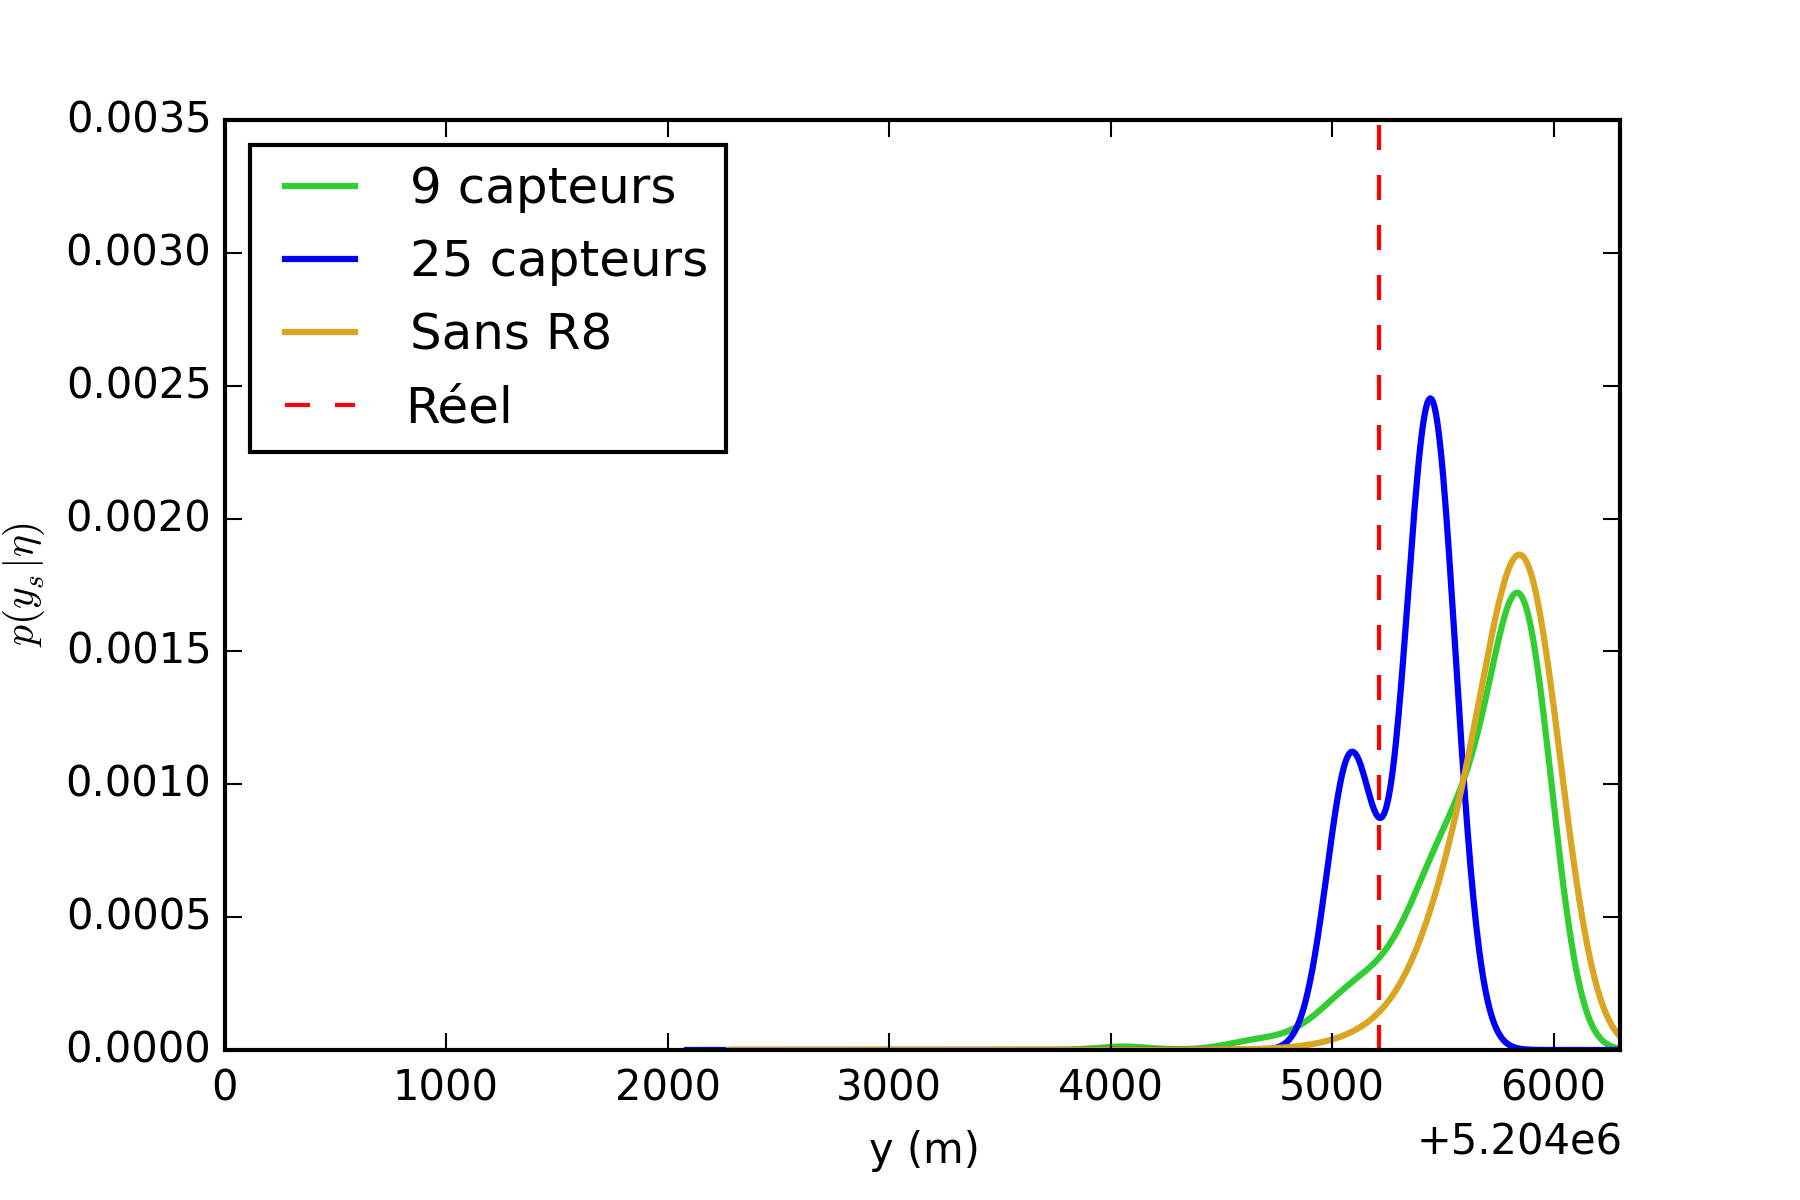
\includegraphics[width=1\textwidth]{kde_y_compare_all.png}
		\caption{}
		\label{kde_y_all}
	\end{subfigure}
	\begin{subfigure}[t]{0.33\textwidth}
		\centering
		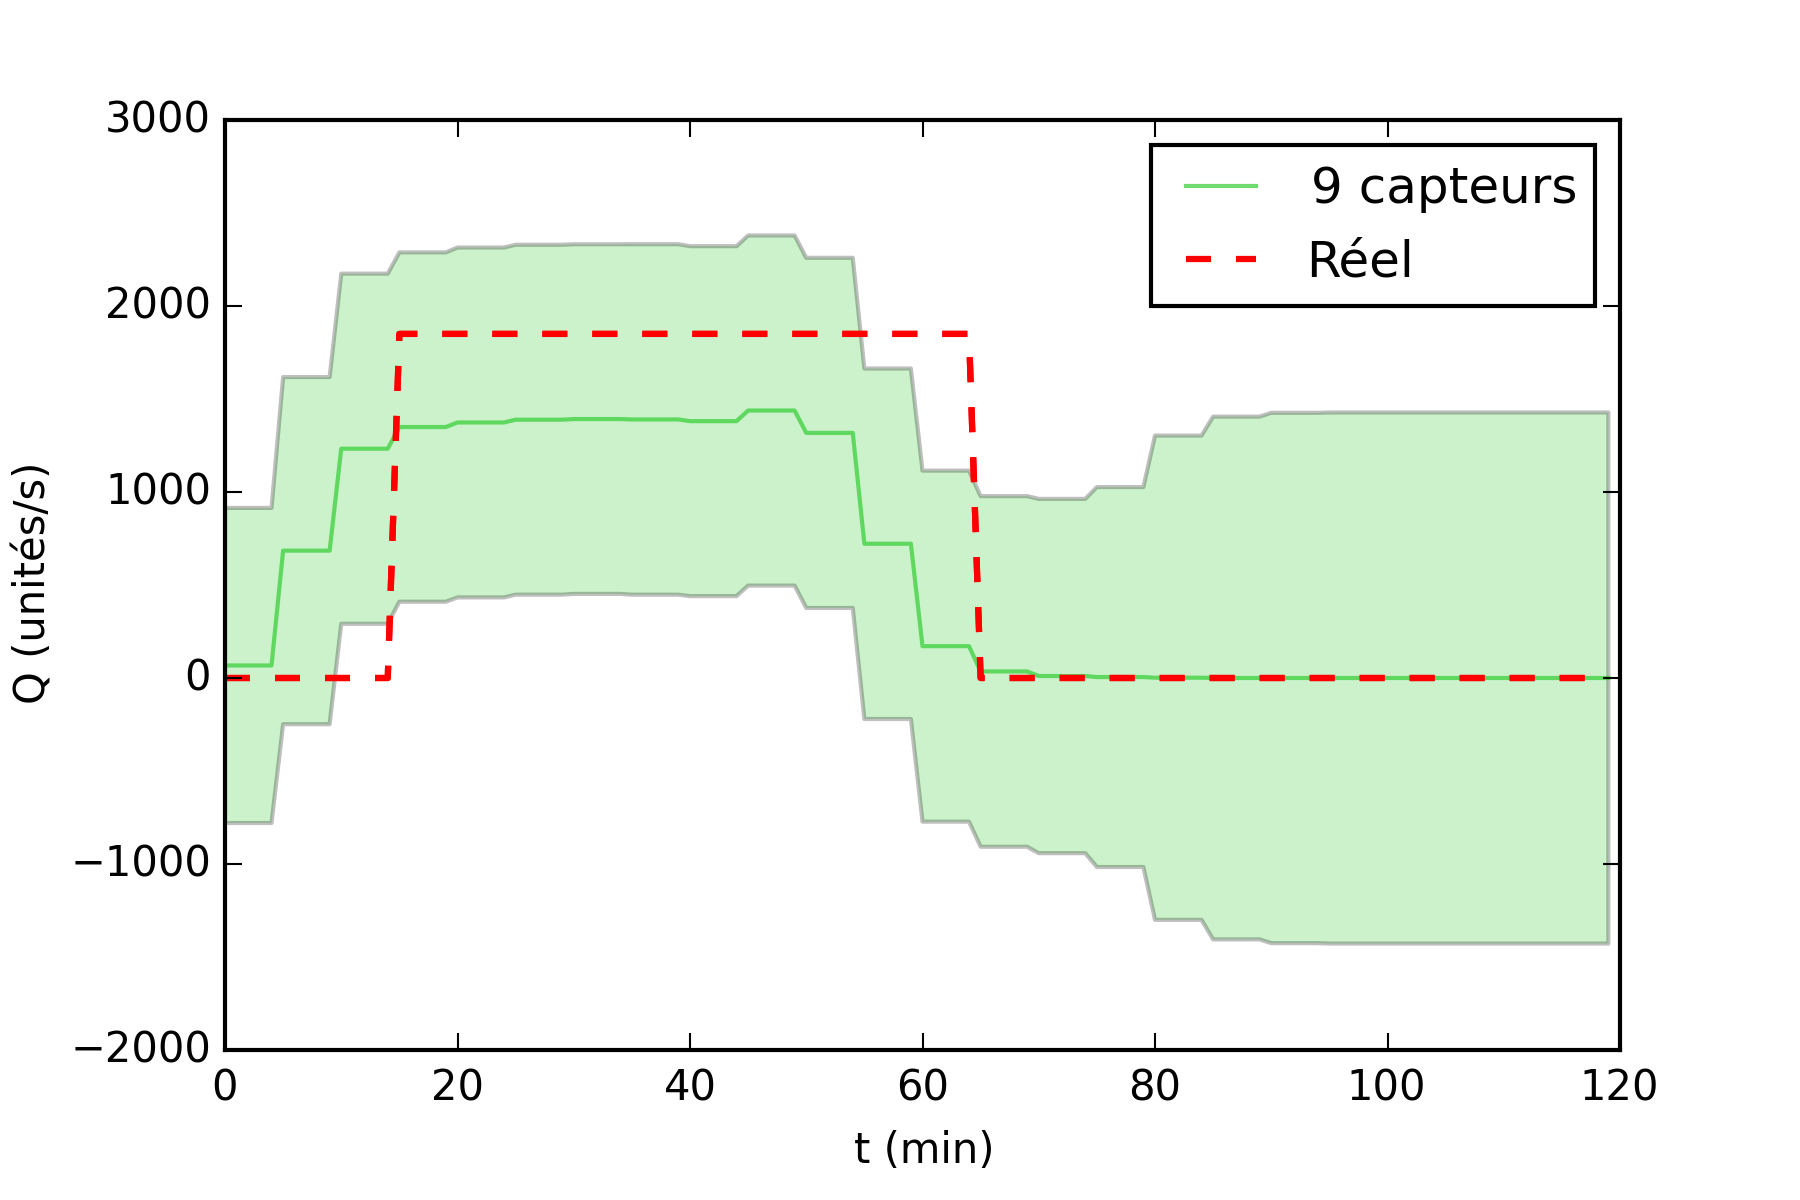
\includegraphics[width=1\textwidth]{q_9C.png}
		\caption{}
		\label{q_9C}
	\end{subfigure}%
	\begin{subfigure}[t]{0.33\textwidth}
		\centering
		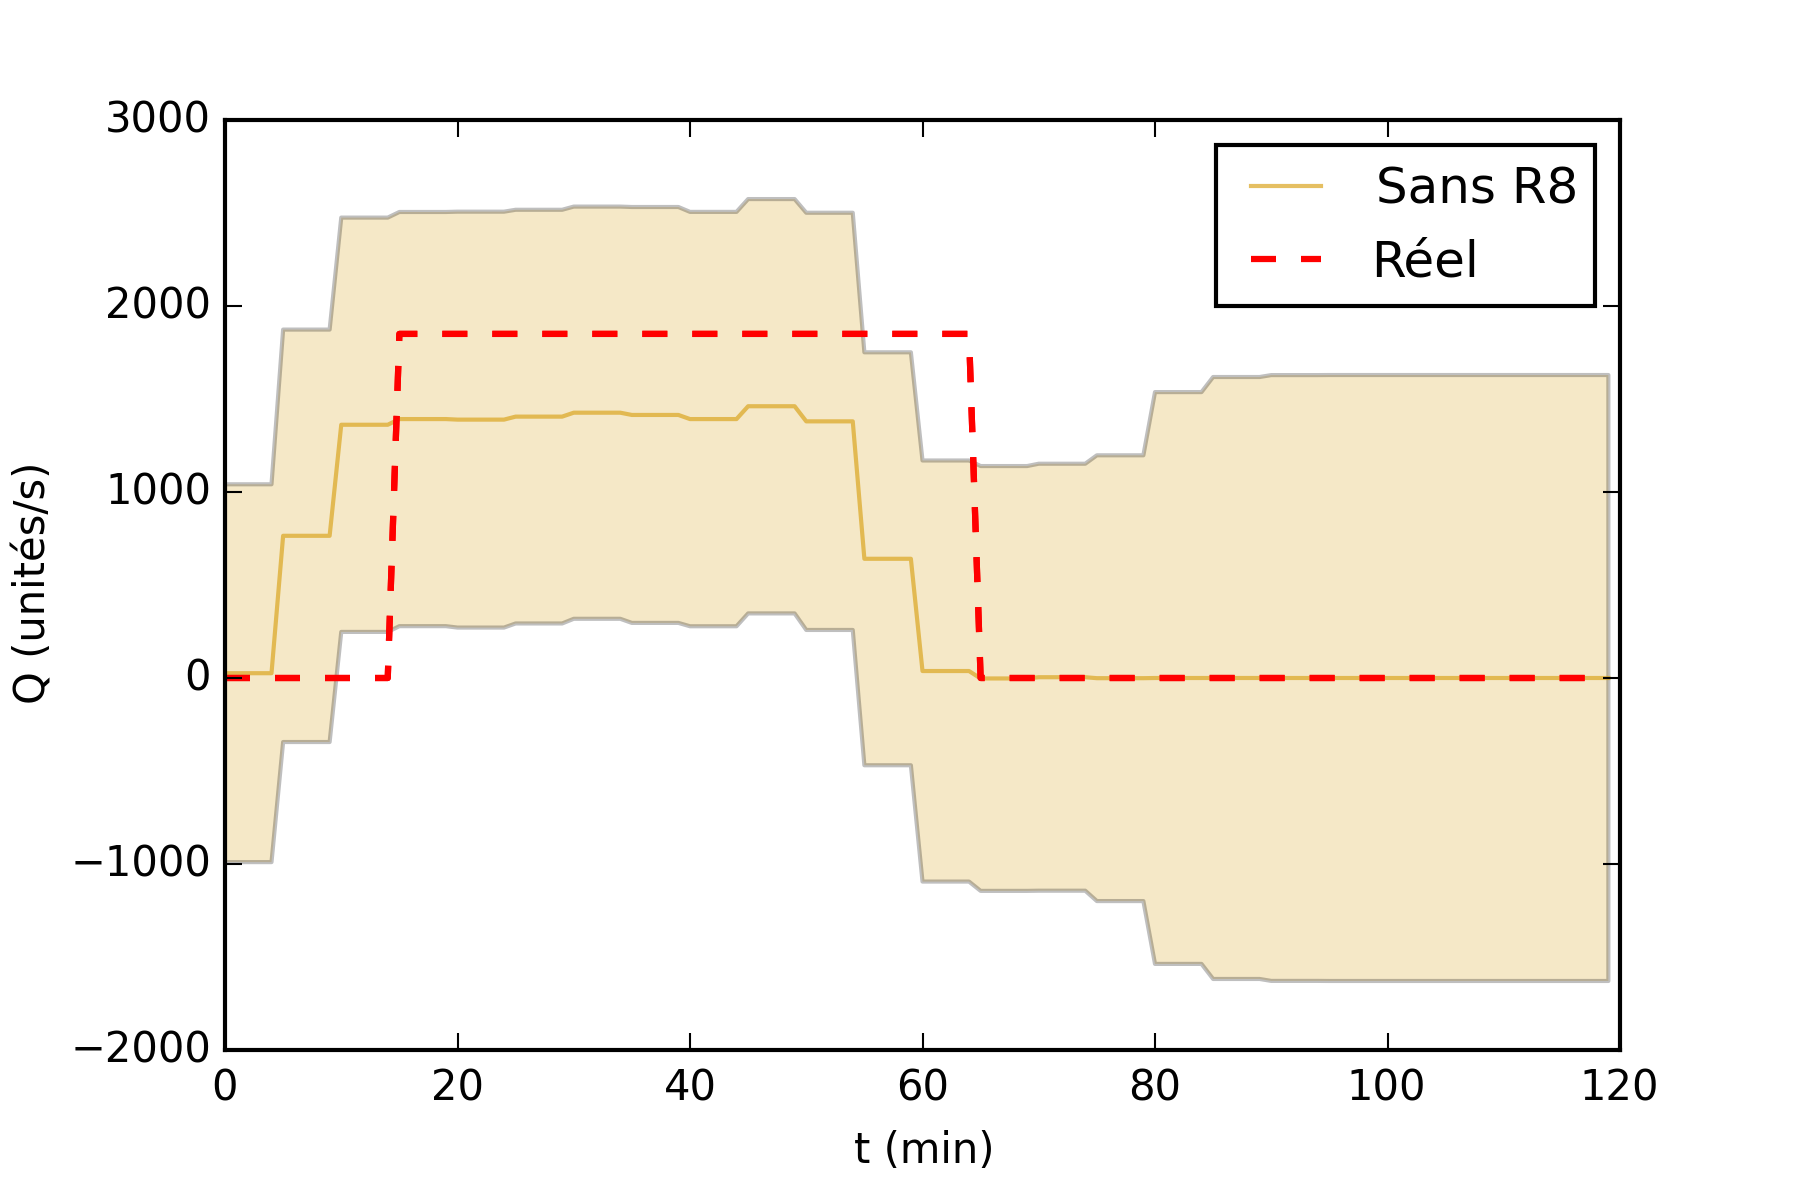
\includegraphics[width=1\textwidth]{q_24C.png}
		\caption{}
		\label{q_24C}
	\end{subfigure}%
	\begin{subfigure}[t]{0.33\textwidth}
		\centering
		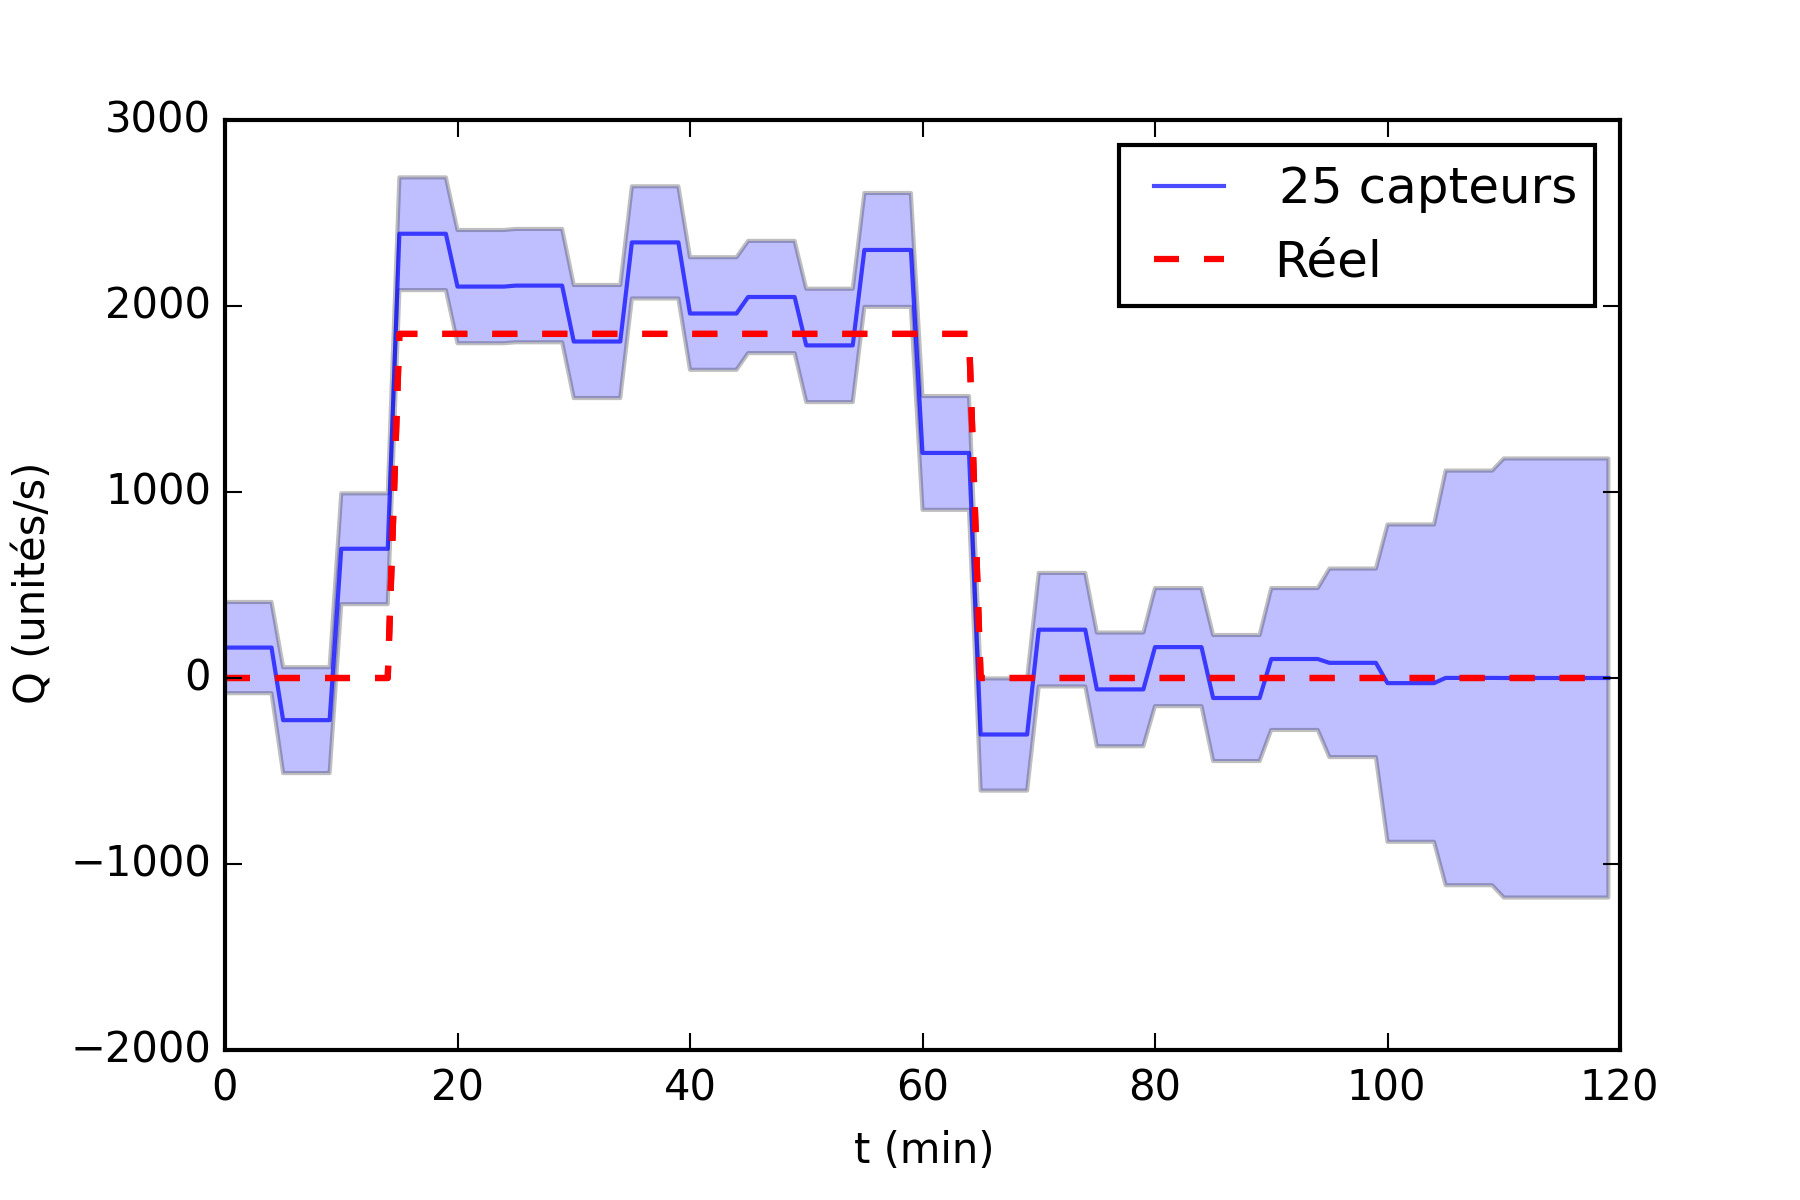
\includegraphics[width=1\textwidth]{q_25C.png}
		\caption{}
		\label{q_25C}
	\end{subfigure}
	\caption{Résultats d'un \textit{run} de l'algorithme d'estimation sans (jaune) et avec (bleu) le capteur R8, comparaison avec un réseau réduit (vert)}
	\label{}
\end{figure}



Les résultats de  localisation de la source montrent une dégradation de l'estimation de la position similaire au cas où le capteur R8 n'est pas présent (figures \ref{kde_x_all} et \ref{kde_y_all}). Il en va de même pour pour l'estimation du profil de rejet (figures \ref{q_9C}, \ref{q_24C} et \ref{q_25C}), où la marge d'incertitude est même légèrement moins grande dans la configuration à capteurs. 

On peut ainsi en déduire que les capteurs n'observant aucune concentration  non-nulle et qui ont été retirés pour établir la configuration à 9 capteurs ont bien un rôle informatif utile au processus d'estimation, et leur apport qualitatif par rapport à la présence du capteur R8 dans le réseau à 25 capteurs semble de même importance.\\

De façon générale, on peut ainsi voir que l'efficacité de l'estimation du terme source repose sur un certain nombre de paramètres d'entrée pour l'algorithme AMIS. Ceux-ci peuvent dépendre entièrement de la configuration du cas-test (nombre de capteur et disposition sur le domaine), ou être définis manuellement par l'utilisateur. Dans ce dernier cas, on a constaté qu'il est difficile d'établir des critères empiriques pour choisir des valeurs par défaut à affecter aux paramètres de variance $\varObs$ et $\varQ$. Pour la variance d'observation, un choix qualitatif a été fait par rapport à l'allure des mesures de la figure \ref{fig_observations_25CAPTEURS}, mais dans d'autres situations pratiques, l'évaluation de $\varObs$ peut se révéler plus compliquée:
\begin{itemize}
	\item si on sait d'avance que certains capteurs du réseau sont plus fiables que d'autres et qu'on choisit d'accorder une plus grande confiance à ces capteurs, alors l'hypothèse d'une loi d'incertitude identiquement distribuée sur les éléments du vecteur d'observation n'est plus valable,
	\item dans un cas opérationnel où on aurait choisi une variance d'observation trop faible, le biais par rapport à la position réelle de la source peut se révéler suffisamment important pour que cette dernière ne soit pas incluse dans l'intervalle de confiance accordé à l'estimation.
\end{itemize}

Pour la variance a priori $\varQ$, le problème est similaire à celui du choix de la matrice d'erreur de \textit{background} en assimilation de données, où la qualité de l'ébauche du terme source fournie influe directement sur la qualité de la reconstruction. 

Une alternative plausible à cette recherche difficile des paramètres initiaux consisterait à travailler sur un ensemble de scénarios possibles, et ainsi d'étudier plusieurs possibilités quant aux valeurs des variances à fournir. Cela demeure possible grâce au gain d'efficacité de calcul permis par l'approche \textit{backward} de l'AMIS, et permettrait d'envisager différents niveaux de confiance accordés aux observation (pour $\varObs$), ainsi que plusieurs hypothèses sur le profil du rejet (pour $\varQ$). Le résultat serait alors un ensemble d'estimations  sur les termes sources possibles selon ces valeurs d'entrée, dont la pertinence serait alors évaluée par les décideurs et les experts en fonction de leur expérience et de la réalité du terrain.




 
 
 




